\documentclass[11pt]{article}
\usepackage{titling}
\usepackage[english]{babel}
\usepackage[margin=0.6in]{geometry} % Page Dimension

%%%%%%%%%%%%%%%%%%%%%%%%%%%%%%%%%%%%%%%%%%
%                PACKAGES                %  
%%%%%%%%%%%%%%%%%%%%%%%%%%%%%%%%%%%%%%%%%%

% Styling Choices
\setlength{\parskip}{\baselineskip}%

% Math
\usepackage{amsmath, amsthm, amssymb}
\usepackage[inline]{asymptote}
\usepackage{xcolor}
\usepackage{cancel}

% Allows for hyperlinking
\usepackage{hyperref}
\hypersetup{
    colorlinks=true,
    linkcolor=magenta,
}

% Blind Footnote
\newcommand\blfootnote[1]{%
  \makeatletter{\footnotetext{#1}\makeatother}
}

% Fancy Header
\usepackage{fancyhdr}
\pagestyle{fancy}
\lhead{Kalda Mechanics}
\rhead{\thepage}

% Coloured Boxes
\usepackage{xcolor}
\definecolor{border}{HTML}{004D4D}
\definecolor{hard}{HTML}{ffccb3}
\definecolor{easy}{HTML}{b3e6b3}
\definecolor{normal}{HTML}{f2f2f2}

% Syntax: \colorboxed[<color model>]{<color specification>}{<math formula>}
\newcommand*{\colorboxed}{}
\def\colorboxed#1#{%
  \colorboxedAux{#1}%
}
\newcommand*{\colorboxedAux}[3]{%
  % #1: optional argument for color model
  % #2: color specification
  % #3: formula
  \begingroup
    \colorlet{cb@saved}{.}%
    \color#1{#2}%
    \boxed{%
      \color{cb@saved}%
      #3%
    }%
  \endgroup
}

% Setup Gray Solution Boxes
\usepackage[breakable,many]{tcolorbox}
\newtcolorbox[auto counter]{solution}[1]{
    enhanced, breakable,
    arc=0pt,
    % colback=default, % Background color
    colframe=white, % Border Color
    coltitle=black, % Title Color
    fonttitle=\bfseries,
    title=\fcolorbox{border}{#1}{\textcolor{border}{pr} \bfseries \textcolor{border}{\thetcbcounter}.},
    attach title to upper,
    after title={\ },
    segmentation style={dashed, gray},
}

% Title and front page
\title{Solutions to Problems in Mechanics Handout by Jaan Kalda With detailed diagrams and walkthroughs}
% Author
\author{\textsc{Ashmit Dutta, QiLin Xue, Kushal Thaman, Arhaan Ahmad}}

\begin{document}
\begin{titlepage}
    \begin{center}
        \vspace*{1cm}
 
        \Huge
        \textbf{Solutions to Jaan Kalda's Problems in Mechanics}
 
        \vspace{0.5cm}
        \LARGE
        \textbf{With detailed diagrams and walkthroughs}
        
        \vspace{0.1cm}
        Edition 1.2.2
        
        \vspace{1.2cm}
 
         Ashmit Dutta, QiLin Xue, Kushal Thaman, Arhaan Ahmad
        \vspace{10mm}
 \begin{center}
\begin{asy}
import olympiad;
size(11cm);
label("N", (1.38, 1.3), NE);
label("$\mu N$", (0.25, 1.15), NW);
label("O", (0,0), W);
label("A", (0.2, 0.2), N);
label("$\theta$", (0.7868, 0.5), 2SW);
label("$\alpha$", (-0.05, -0.6), SE);
label("$\beta$", (0.7, -2.3), N);

draw(circle((0,0), 1), linewidth(1.5pt));
filldraw(circle((0.2, 0.2), 0.72), gray(0.9));
dot((0,0));
dot((0.2,0.2));
draw((0.25, -0.954)--(0.7868, -3), linewidth(1.5pt));
filldraw(circle((0.7868,-3), 0.1), black);
draw((0,0)--(0,-3), dashed);
draw((0,0)--(0.7868, -3));
draw((0.2,0.2)--(0.7868,-3), dotted);
draw((0.7868, 0.6172)--(0.7868, -3), dashed);
draw((0, 0)--(0.7868, 0.6172));
draw((0.7868, 0.6172)--(0.25, 1.15), arrow=Arrow(4));
draw((0.7868, 0.6172)--(1.38, 1.3), arrow=Arrow(4));
draw((0.7868, 0.6172)--(0.7868, 1.8), arrow=Arrow(4));
label("Q", (0.7868, 1.8), N);

pair A,B,C,D,E,F,G, H;
B = (0.7868, -3);
A = (0,0);
C = (0.2, 0.2);
D = (0, -3);
E = (0.7868, 2.1);
F = (-0.5, 1.9);
G = (0.7868, 0.6172);
H = (0.7868, -3);
markscalefactor=0.05;
draw(anglemark(E, G, F, 4));
draw(anglemark(A, G, H, 4));
markscalefactor=0.1;
draw(anglemark(D, A, B, 4));
draw(anglemark(G, H, A, 4));
\end{asy}
\end{center}
        \vfill
        
        \Large
        Updated
        \today
 
    \end{center}
\end{titlepage}
\newpage
%%%%%%%%%%%
% Preface %
%%%%%%%%%%%
\section*{Preface}
\vspace{-5mm}
\indent Jaan Kalda's \href{https://www.ioc.ee/~kalda/ipho/}{handouts} are beloved by physics students both in for a quick challenge, to students preparing for international Olympiads. As of writing, the current \href{https://www.ioc.ee/~kalda/ipho/meh_ENG2.pdf}{mechanics} handout (ver 1.2) has 86 unique problems and 74 main `ideas'.

This solutions manual came as a pilot project from the online community at \url{artofproblemsolving.com}. Although there were detailed hints provided, full solutions have never been written. The majority of the solutions seen here were written on a private forum given to those who wanted to participate in making solutions. In an amazing show of an online collaboration, students from around the world came together to discuss ideas and methods and created what we see today.

This project would not have been possible without the countless contributions from members of the community. Online usernames were used for those who did not wish to be named: 

\textit{Heramb Podar, Ameya Deshmukh, Viraj Jayam, Rakshit, dbs27, Anant Lunia, Jai, Sean Chen, Ayon Ghosh, Joshua S, Tarun Agarwal, c\_deng}
\subsection*{Structure of The Solutions Manual}
\vspace{-5mm}
Each chapter in this solutions manual will be directed towards a section given in Kalda's mechanics handout. There are three major chapters: statics, dynamics, and revision problems. If you are stuck on a problem, cannot make progress even with the hint, and come here for reference, look at only the start of the solution, then try again. Looking at the entire solution wastes the problem for you and ruins an opportunity for yourself to improve.

\subsection*{Contact Us}
\vspace{-5mm}
Despite editing, there is almost zero probability that there are \textit{no} mistakes inside this book. If there are any mistakes, you want to add a remark, have a unique solution, or know the source of a specific problem, then please contact us at \url{hello@physoly.tech}. The most current and updated version can be found on our website \url{physoly.tech}

Please feel free to contact us at the same email if you are confused on a solution. Chances are that many others will have the same question as you.

\newpage
\section{Solutions to Statics Problems}
\vspace{-5mm}
This section will consist of the solutions to problems from problem 1-23 of the handout. Statics is typically the analysis of objects not in motion. However, objects travelling at constant velocity or with a uniform acceleration can be treated as a statics problem with a frame of reference change. This usually involves balancing forces, torques, and more to achieve equilibrium. 

\begin{solution}{normal}
Applying idea 1, we have:
$$P=C\frac{dT}{dt}$$
where
$$\frac{dT}{dt}=\frac{aT_0}{4}(1+a(t-t_0))^{-3/4}$$
Since we have that,
\[T(t) = T_0 [1 + a(t -t_0)]^{1/4}\]
dividing by $T_0$ gives us 
\[\frac{T}{T_0} = [1 + a(t - t_0)]^{1/4}.\]
We then get 
$$\frac{dT}{dt}=T_0^4(a/4)(1/T^3)$$
Plugging everything back in, we get:
$$\boxed{C=\frac{4PT^3}{aT_0^4}}$$
\end{solution}
\begin{solution}{normal}
The ice melts when the temperature of the kettle begins to drop. All the heat that was supplied to the kettle was used in melting the ice and bringing it up to the temperature of the rest of the water. Meanwhile the water already present lost some heat to the surroundings, and thus the graph dips at that point.
\vspace{3mm}

The total time for the temperature to recover to $T = 75^{\circ}\;\mathrm{C}$ is approximately $t = 37\;\mathrm{s}$. The heating rate of water is the slope of the graph or $dT/dt$. This means that the power at $T = 70^{\circ}\;\mathrm{C}$ is $P' = P \tan 75^{\circ}\approx 500\;\mathrm{W}$. Therefore, from energy conservation, we have that 
\[mL + mc\Delta T = Pt\implies m = \frac{Pt}{L + c\Delta T} \approx \boxed{28\;\mathrm{g}}.\]
\end{solution}
\begin{custom-simple}[Problem 3]
If the light is coherent, then the amplitude of the light emerging from each slit can individually be written as:
$$E=E_0\cos(\omega t + \phi)$$
where $\omega$ is the frequency and $\phi$ is the phase shift. An alternative way of writing this is:
$$E=E_0e^{i\omega t}e^{i\phi}$$
Its real component corresponds with the magnitude of the field that we measure at a certain time $t$. The complex number $e^{i\omega t}e^{i\phi}$ can be represented as a phasor which is essentially a vector with a constant magnitude of one that rotates in the complex plane at an angular frequency of $\omega$ (that is, it makes an angle $\omega t+\phi$ with the real axis). We want the sum of the three different amplitudes to sum up to zero, or:
$$E_1+E_2+E_3=E_0\cdot \left[e^{i\omega t}e^{i\phi_1}+e^{i\omega t}e^{i\phi_2}+e^{i\omega t}e^{i\phi_3}\right] = 0$$
Although this may look complicated, we can simplify it by treating them geometrically as phasors. To achieve an intensity minima of zero, we need three phasors such that their vector sum equals zero, which is equivalent to making a closed shape. Since they have the same magnitude, this shape must be an equilateral triangle. Without loss of generality, let $\phi_1=0$. This means $\phi_2=\phi_3=2\pi k + \frac{2\pi}{3}$ where $k$ is an integer.

The phase shift is defined as:
$$\frac{\phi}{2\pi} = \frac{(\text{path difference})}{\lambda} \implies k+ \frac{1}{3} = \frac{d\sin\theta}{\lambda}$$
where $d$ is the separation between two arbitrary slits and $\theta$ is the angle the light makes with the horizontal. Applying this for the slit separation distances in this problem, we have:
$$a = \left(k_1+\frac{1}{3}\right)\frac{\lambda}{\sin\theta_1}$$
$$b = \left(k_2+\frac{1}{3}\right)\frac{\lambda}{\sin\theta_2}$$
If we assume that $a,b \ll L$ where $L$ is the distance between the slits and the screen, then $\sin\theta_1=\sin\theta_2$. Taking the ratio, we get:
$$\frac{a}{b} = \frac{n}{m} \equiv \frac{3k_1+1}{3k_2+1}$$
This produces a minima of zero for any integer combinations of $k_1$ and $k_2$. We will prove that for each combination, $n-m$ is a multiple of three. We have:
$$3k_2+1 - (3k_2+1) = 3r \implies 3(k_2-k_1)=3r \implies k_2-k_1=r$$
where $r$ is an integer. Since $k_1$ and $k_2$ have to be integers, then $r$ must also be an integer, proving the statement.
\end{custom-simple}
\begin{solution}{easy}
Applying fact 6, we find that the initial heat flux is proportional to $\Delta T_1 = T_1 - T_0$ as the temperature change is minimal (in fact smaller than one Kelvin). Likewise, the final heat flux is proportional to $\Delta T_2 = T_2 - T_0$. Therefore, we have that the ratio of powers is \[\frac {P + P_{\text{man}}}{P} = \frac {\Delta T_2}{\Delta T_1}\]
Solving for $P_{\text{man}}$ and plugging in our numbers, we find that \[P_{\text{man}}= P\left(\frac {T_2-T_1}{T_1}\right) = \boxed{52.6\;\mathrm{W}}.\]
\end{solution}
\begin{solution}{easy}
\begin{center}
    \begin{asy}
    size(5cm);
draw((0,0)--(0,1)--(1,1)--(1,0)--cycle);
draw((0.5,0.5)--(0.25,0.5), arrow=Arrow(4));
label("$v$", (0.25, 0.5), W);
draw((0.5,0.5)--(0.5,0.75), arrow = Arrow(4));
label("$u$", (0.5, 0.75), E);
draw((0.5,0.5)--(0.75,0.25), arrow=Arrow(4));
label("$F_f$", (0.75, 0.25), SE);
    \end{asy}
\end{center}
In the board's frame of reference, there is only a horizontal force (the friction force), which has a constant direction that is anti-parallel to the velocity. Thus, the chalk moves in a $\boxed{\text{straight line}}$.
\end{solution}
\begin{solution}{hard}
a) We examine the forces involved in a cross-section of the cylinder. Assuming the block behaves like a point mass, and noting there is a centrifugal force, we create following diagram
\begin{center}
\begin{asy}
import olympiad;
size(5cm);
draw(circle((0,0), 1));
dot((sqrt(2)/2, sqrt(2)/2));
draw((sqrt(2)/2, sqrt(2)/2)--(0,0), arrow=Arrow(4));
draw((sqrt(2)/2, sqrt(2)/2)--(1.15, 1.15), arrow=Arrow(4));
draw((sqrt(2)/2, sqrt(2)/2)--(sqrt(2)/2, 0), arrow=Arrow(4));
draw((sqrt(2)/2, sqrt(2)/2)--(sqrt(2)/2+0.5, sqrt(2)/2-0.5), dotted, arrow=Arrow(4));
draw((sqrt(2)/2, sqrt(2)/2)--(sqrt(2)/2-0.5, sqrt(2)/2+0.5), arrow=Arrow(4));
draw((sqrt(2)/2, sqrt(2)/2)--(sqrt(2)/2, 0), dotted);
draw((0,0)--(sqrt(2)/2, 0), dotted);
draw((sqrt(2)/2, sqrt(2)/2)--(sqrt(2)/2+0.5, sqrt(2)/2), dotted);

pair A,B,C,D,E,F, G;
B = (sqrt(2)/2, sqrt(2)/2);
A = (sqrt(2)/2-0.5, sqrt(2)/2+0.5);
C = (sqrt(2)/2, 1.3);
D = (0, 0);
E = (sqrt(2)/2, 0);
F = (sqrt(2)/2+0.3, sqrt(2)/2);
G = (sqrt(2)/2+0.5, sqrt(2)/2-0.5);

draw(anglemark(G, B, F, 4));
draw(anglemark(E, D, B, 4));

label("$\theta$", (0.1, -0.05), NE);
label("$\theta$", (sqrt(2)/2+0.1, sqrt(2)/2+0.05), SE);
label("N", (0, 0), SW);
label("$\mu N$", (sqrt(2)/2-0.5, sqrt(2)/2+0.5), NW);
label("$mg$", (sqrt(2)/2, 0), S);
label("$m\omega^2 r$", (1.15, 1.15), NE);
\end{asy}
\end{center}
Because the system is in equilibrium we must set the resultant force to be zero in both directions. We assume a tilted coordinate of $\theta$ to perform our calculations on. In the vertical direction we have
\[0=N+mg\sin\theta-m\omega^2 r\]this in turn implies that the normal force is
\[N=m\omega^2 r-mg\sin\theta.\]Looking in the horizontal direction we note that
\[\mu N-mg\cos\theta=0\]\[mg\cos\theta=\mu N\]However, we remember that $\mu N$ is the maximum amount of friction obtained from slipping, thus we have to put a less than or equal sign to obtain
\[mg\cos\theta\leq\mu N\]substituting in $N$ from our previous calculation we have
\[mg\cos\theta\leq\mu(m\omega^2 r-mg\sin\theta)\]moving variables to the other side and canceling out $m$ gives
\[\omega^2 r\geq g(\mu^{-1}\cos\theta+\sin\theta)\]Our goal is to now to find a maximal value of $\mu^{-1}\cos\theta+\sin\theta$ on the interval $[0, 2\pi]$. It is known that a sinusoid $A\cos\theta+B\sin\theta$, can be represented as a single trigonometric function: $$A\cos\theta+B\sin\theta=\sqrt{A^2+B^2}\cdot\cos{(\theta + \phi)}$$
From these expressions of 1 sinusoid, it is clear the maximum value is $\sqrt{A^2+B^2}$, giving the maximum of $\mu^{-1}\cos\theta+\sin\theta$ as $\sqrt{1+\mu^{-2}}.$ Thus replacing this value in for our final expression gives us
\[\boxed{\omega^2 r\geq g(\sqrt{\mu^{-2}+1})}\]
b) In this part we work with cylindrical coordinates. We decompose gravity upon two axes. If we rotate the cylinder by $\alpha$ we have
\begin{align*}
g_{z}=g\sin\alpha\\ 
g_{r,\theta}=g\cos\alpha
\end{align*}All we do now is plug in $g_{\text{eff}}$ for our two equations. For our radial equation we had
\[N=m\omega^2 r-mg\sin\theta\]Since the normal force is radial we use $g_{r,\theta}=g\cos\alpha$ we plug in for gravity to get
\[N=m\omega^2 r-mg\cos\alpha\sin\theta\]In our second equation who have two components of gravity, $F_{\theta}$ and $F_z$, who’s combined modulus must be less than friction or $\mu N$.
\[\sqrt{F_{\theta}^2+F_r^2}\leq\mu N\]\[\sqrt{(mg\cos\alpha\cos\theta)^2+(mg\sin\alpha)^2}\leq\mu(m\omega^2 r-mg\cos\alpha\sin\theta)\]Taking out $m$ and factoring we have
\[\boxed{\omega^2 r\geq g\cos\alpha(\sqrt{\cos^2\theta+\tan^2\alpha}+\mu\sin\theta)}\]Again we must maximize our right hand equation. Inevitably, there is no neat trick to maximize this apart from differentiating and setting the result to zero.
\end{solution}

\begin{solution}{hard}
\begin{center}
    \begin{asy}
    size(8.5cm);
        import olympiad;
        pair A, B, C, D;
        A = (0,0);
        B = (2, 1);
        C = (2, 0);
        D = (2, -0.5);
        
        dot(A);
        draw(A -- B, arrow = Arrow(4));
        draw(A -- C, arrow = Arrow(4));
        draw("$v\cos\alpha$", A -- (1, 0), 2SE, arrow = Arrow(4));
        draw(B -- D, dashed);
        draw(anglemark(C, A, B));
        draw((2.6, 1) -- (2.6, -0.5), arrow=Arrow(4));
        
        /*labels and dots*/
        label("$\alpha$", (0.3, 0.01) , NE);
        label("$v$", B, N);
        label("$\frac{uL}{v\cos\alpha}$", (2, 0.6), E);
        label("$ut$", (2.6, 0.25), E);
        label("$s$", (2, -0.25), E);
    \end{asy}
\end{center}
Denote the dashed line by the wall which is a distance $L$ away from the point source.\vspace{3mm}

We express the lateral displacement of the ball as the sum of two components: lateral displacement in the air’s frame of reference, and the lateral displacement of the moving frame.\vspace{3mm}

In the air's frame the displacement is given by 
\[ut_{\text{air}} = \frac{uL}{v\cos\alpha}\]
and the lateral displacement in the moving frame is given by $s$. This gives us 
\[ut = \frac{uL}{v\cos\alpha} + s\implies t = \boxed{\frac{s}{u} + \frac{L}{v\cos\alpha}}\]
\end{solution}
\begin{solution}{hard}
\textbf{a)} Let the point where the rope meets the cylinder be $A$, and the two points where friction band meets the cylinder be $B$ and $C$. Let $D$ be the point diagonally opposite $A$.
\vspace{2mm}

\textbf{\textcolor[HTML]{3D85C6}{Claim.}} $D$ is the instantaneous centre of rotation (ICOR).
\begin{center}
\begin{asy}
size(5cm);
draw(circle((0,0), 1));
dot((0,1));
label("A", (0,1), N);
dot ((0,-1));
label("D", (0,-1), S);
draw((-sqrt(2)/2, sqrt(2)/2)--(sqrt(2)/2, sqrt(2)/2));
draw((-sqrt(2)/2-0.09, sqrt(2)/2-0.1)--(sqrt(2)/2+0.09, sqrt(2)/2-0.1));
label("B", (-sqrt(2)/2-0.09, sqrt(2)/2-0.1), NW);
label("C", (sqrt(2)/2+0.09, sqrt(2)/2-0.1), NE);
\end{asy}
\end{center}
\begin{proof} Let us assume a contradictory case. Let $D^*$ be the ICOR. Since the velocity of point $A$ is perpendicular to $AD$, $D^*$ must lie somewhere on $AD$. The velocities of $B$ and $C$ are perpendicular to $DB$ and $DC$ (due to definition of ICOR), and the friction forces are anti-parallel to these. The only forces acting on the cylinder is the tension $T$ due to the rope, and the two friction forces. As the cylinder is in equilibrium, by setting torque to be $0$ about the point where the two friction vectors intersect, we see that the tension vector must also pass through it. However, due to symmetry, the point of intersection must lie on $AD$ and thus it must be $A$ itself.
Thus, $\angle ABD^* = \angle ACD^* = 90^{\circ}$. Therefore this means that $ABCD^*$ is cyclic, which implies $D^* \equiv D$.
\end{proof}
\vspace{3mm}

Now let the angular velocity about $D$ be $\omega$. The velocity of $A$  is
$$v =\omega \times 2R$$
and the velocity at the centre is:
$$\boxed{v_\text{center}= \omega \times R = \frac{v}{2}}$$
\vspace{2mm}

\textbf{b)} Dividing the floor into various infinitesimally thin strips like in $a)$, we can conclude that the ICOR is still $D$ and the answer remains the same.
\end{solution}

\begin{solution}{normal}
Let us assume that $-dm'$ mass sublimes at some instant. ($m'$ is the total mass of the cup.)
Intially it is moving with $v$, the velocity of the vessel
Finally its velocity \textit{with respect to the vessel}, in the \textit{direction of motion} of the vessel becomes $-\frac{\sqrt {\frac{3RT}{\mu}}}{\sqrt 3}=-\sqrt{\frac{RT}{\mu}}.$\footnote{Since the rms speed is randomly directed in $x, y, z$ directions and we only want one speed, we divide by the magnitude of the unit vectors.}
Thus, it provides an impulse, $-(-dm' \Delta v )= -dm'\sqrt{\frac{RT}{\mu}}$ to the vessel
$$\therefore v = \int dv=\int_{M+m}^{M}\frac{-dm'\sqrt{\frac{RT}{\mu}}}{m'}=\sqrt{\frac{RT}{\mu}}\textup{ln}\left (1+\frac{m}{M}  \right )\approx \boxed{\sqrt{\frac{RT}{\mu}}\frac{m}{M}} $$
\end{solution}
\begin{solution}{normal}
\begin{center}
\begin{asy}
/* Geogebra to Asymptote conversion, documentation at artofproblemsolving.com/Wiki go to User:Azjps/geogebra */
import graph; size(5cm);
real labelscalefactor = 0.5; /* changes label-to-point distance */
pen dps = linewidth(0.7) + fontsize(10); defaultpen(dps); /* default pen style */
pen dotstyle = black; /* point style */
real xmin = -4.23213963380496, xmax = 7.371171204866221, ymin = -1.6441239198422954, ymax = 4.437435927619134; /* image dimensions */

/* draw figures */
draw((0,0)--(3,0), linetype("2 2"));
draw((3,0)--(3,4), linetype("2 2"));
draw((3,4)--(0,0), linetype("2 2"));
draw((0,0)--(2,0),EndArrow(6));
draw((2,0)--(2,2.7), EndArrow(6));
label("$\ell$",(1.37,2.6),SE*labelscalefactor);
label("$\mu N$",(0.823,0.4),SE*labelscalefactor);
label("$N$",(1.6,1.43),SE*labelscalefactor);
label("$h$",(3.15,2.22),SE*labelscalefactor);
label("$\sqrt{\ell^2-h^2}$",(1.2,-0.1),SE*labelscalefactor);
/* dots and labels */
dot((0,0),dotstyle);
label("$A$", (0,0), SW * labelscalefactor);
dot((3,0),dotstyle);
label("$B$", (3,0), NE * labelscalefactor);
dot((3,4),dotstyle);
label("$C$", (3,4), NE * labelscalefactor);
clip((xmin,ymin)--(xmin,ymax)--(xmax,ymax)--(xmax,ymin)--cycle);
/* end of picture */
\end{asy}
\end{center}
Consider what happens when the applied force approaches infinity. To maintain equilibrium, the friction force between the rod and the board must also increase. This friction force will also approach infinity. When dealing with large forces, we can ignore constant forces such as the weight of both the board and the rod.
\vspace{2mm}

As a result, since the weight of the rod is negligible we can pretend it's a mass-less rod. We also know that the forces at the ends of a massless rod will always point along the rod. For example, the force exerted on the rod by the board must point along the rod as well. The angle of this force is solely dependent on the friction coefficient $\mu_1$. Therefore:
$$\tan\alpha < \frac{\mu_1 N}{N} \implies \boxed{\mu_1>\frac{\sqrt{\ell^2-h^2}}{h}}$$
\tcbline
\textbf{Solution 2:} We want that when the board is on the verge of slipping then the rod should exert a larger force on the board (the rod should be pulled towards the board and not away from it). Consider the torque on the rod about the hinge point. We want that it should be clockwise when the block is on the verge of slipping.
\vspace{2mm}

Let the sum of normal reaction and friction force on the rod be $f$ (the normal points upwards and the friction points to the right). When the block is on the verge of slipping, the resultant makes an angle $\tan^{-1} \mu$ from the normal. We have:
$$\tau = mg\sin \alpha\frac{l}{2} + f \sin (\tan^{-1} \mu - \alpha)$$
considering clockwise torque to be positive. As the applied force on the block increases, $f$ also increases without bounds and because we want the torque to be clockwise no matter how much force we apply, the $mg$ term can be neglected. So
$$f \sin(\tan^{-1}\mu-\alpha) \ge 0$$
Since both $\tan^{-1}\mu$ and $\alpha$ are less than $90^{\circ}$, we can conclude that
$$\boxed{\tan^{-1} \mu \ge \alpha \implies \mu \ge \frac{\sqrt{l^2-h^2}}{h}}$$
\end{solution}

\begin{solution}{hard}
Let us divide the displacement into tiny pieces, $s=\sum\Delta s$ where $\Delta s = v\Delta t$. \vspace{3mm} 

If the function $v(t)$ were known, the last formula would have been completed our task, because $\sum v(t)\Delta t$ is the sum of rectangles making up the area under the $v-t$-graph. \vspace{3mm}

However, the acceleration is given to us as a function of $v$, hence we need to substitute $\Delta t$ with $\Delta v$. \vspace{3mm}

While trying to do that, we can introduce the acceleration (which is given to as a function of $v$):
\[\Delta t = \Delta v\cdot \frac{\Delta t}{\Delta v} = \frac{\Delta v}{\Delta v/\Delta t} = \frac{\Delta v}{a}.\]
In other words
\[s = \sum \frac{v}{a}\Delta v = \int \frac{v}{a(v)}dv.\]This tells us that the answer is equal to the area under a graph which depicts $\dfrac{v}{a(v)}$ as a function of $v$.\vspace{3mm}

Applying a \href{https://www.wolframalpha.com/input/?i=fit+\%7B0\%2C0\%7D\%2C\%7B2\%2C0.2\%7D\%2C\%7B3.1\%2C0.4\%7D\%2C\%7B4\%2C0.8\%7D\%2C\%7B3.3\%2C0.46\%7D\%2C\%7B2.3\%2C0.24\%7D\%2C\%7B2.4\%2C0.26\%7D\%2C\%7B0.7\%2C0.06\%7D\%2C\%7B1.7\%2C0.16\%7D\%2C\%7B0.5\%2C0.04\%7D}{quartic least-squares} fit to some of the discernible data points, we can see that the curve $a(v)$ is well approximated by the function $0.00617211 v^4 - 0.0301639 v^3 + 0.0581573 v^2 + 0.0546369 v + 0.000715828$.\vspace{3mm}

Taking the \href{https://www.wolframalpha.com/input/?i=integral+from+0+to+4+of+x\%2F\%280.00617211+x\%5E4+-+0.0301639+x\%5E3+\%2B+0.0581573+x\%5E2+\%2B+0.0546369+x+\%2B+0.000715828\%29}{integral}, we can see that
\begin{align*}
    \int_0^4\dfrac{v}{a(v)}dv&\approx\int_0^4\dfrac{v}{0.00617211 v^4 - 0.0301639 v^3 + 0.0581573 v^2 + 0.0546369 v + 0.000715828}dv\\
    &\approx \boxed{39\;\text{m}}
\end{align*}
\blfootnote{Don't worry if your answer isn't exactly the same as ours, as this result may be difficult to determine by hand with the graph provided. A rough approximation (within reasonable limits) would suffice.}
\end{solution}
\begin{solution}{normal}
First, we'll look at the behavior of the tension at the bottom. The vertical component of the tension has to support the weight of the block so we have:
$$2T_\text{bottom,y} = 2T_\text{bottom}\cos(\beta/2) = Mg$$The horizontal component is thus:
$$T_x=T_\text{bottom}\sin(\beta/2) = \frac{Mg}{2}\tan(\beta/2)$$Notice that this horizontal tension force will be constant in a massive rope. If we look at a differential area of the string, the only other force other than tension is the gravitational force downwards. To balance horizontal forces, the horizontal components of tension have to be constant. At the top of the rope, the vertical component of the tension has to support the weight of the block and the string. We have:
$$2T_\text{top,y} = 2T_\text{top}\sin\alpha = (M+m)g$$The horizontal component will thus be:
$$T_x = T_\text{top}\cos\alpha = \frac{(M+m)g}{2}\cot\alpha$$
Setting these two expressions for the horizontal tension equal gives:
$$M\tan(\beta/2)=(M+m)\cot\alpha \implies \boxed{\beta = 2 \tan^{-1}\left(\left(1+\frac{m}{M}\right)\cot \alpha\right)}$$
\end{solution}

\begin{solution}{normal}
The total mass of the balloon is $Mg + m_{H_2} g$ which is equal to the mass of the air that is holding the balloon up $\rho_{\text{air}} Vg$. From the ideal gas law, we can write 
\[\rho_{\text{air}} = \frac{p\mu_{\text{air}}}{RT_{\text{air}}}\]
and similarly, we can write the mass of the hydrogen gas $m_{H_2}$ as 
\[m_{H_2} = \frac{p\mu_{H_2}V}{RT_{\text{air}}}.\]
We can then write that 
\[\rho_{\text{air}} Vg = Mg + m_{H_2} g\implies  \frac{p\mu_{\text{air}}}{RT_{\text{air}}}Vg = Mg + \frac{p\mu_{H_2}V}{RT_{\text{air}}}g.\]
This means that 
\[M_0 =  \frac{pV_0}{RT_{\text{air}}} (\mu_{\text{air}} - \mu_{H_2}).\]
The mass of the balloon when it reaches a volume $V_1$ is then given by 
\[M_1 =  \frac{pV_1}{RT_{\text{air}}} (\mu_{\text{air}} - \mu_{H_2})\]
and by Charle's law, note that 
\[\frac{V_1}{T_{\text{air}}} = \frac{V_0}{T_1}\]
which means that
\[M_1 =  \frac{pV_0}{RT_1} (\mu_{\text{air}} - \mu_{H_2}).\]
The ballast needed to be thrown out is then 
\[\Delta m = M_0 - M_1 = (\mu_{\text{air}} - \mu_{H_2})\frac{pV_0}{R}\left(\frac{1}{T_{\text{air}}} - \frac{1}{T_1}\right).\]
\end{solution}
\begin{solution}{normal}
\begin{center}
    \begin{asy}
        unitsize(3cm);
        pair O = (0,0);
        pair A = (1,1);
        pair B = (2,-0.5);
        draw(O--A--A+B--B--O--B--B+(1,0.3)--A+B);
        draw(arc(B,0.3,16,45));
        label("$\alpha$",B+(0.38,0.22));
        draw(B/2-(1,0)--B/2,arrow=Arrow());
        draw(arc(B/2,0.5,180,166));
        label("$\beta$",B/2-(0.8,-0.08));
        draw(ellipse(B/2-(1.2,0.05),0.2,0.2/3));
        filldraw(B/2-(1,0.05)--B/2-(1.4,0.05)--B/2-(1.4,-0.05)--B/2-(1,-0.05)--cycle,gray(0.949),invisible);
        draw(ellipse(B/2-(1.2,-0.05),0.2,0.2/3));
        draw(B/2-(1,-0.05)--B/2-(1,0.05));
        draw(B/2-(1.4,-0.05)--B/2-(1.4,0.05));
        label("$v_0$",B/2+(-0.6,-0.1));
    \end{asy}
\end{center}

When on the plane, the puck experiences no change in its x-velocity, which is
$$v_0\cos\beta=5\;\text{m/s}$$

However, it experiences an acceleration parallel to the plane with magnitude
$$a=g\sin\alpha$$

We note from the trajectory given that the puck drops $2.5\;\text{m}$ below the apex of its trajectory while undergoing a horizontal displacement of $x=5\;\text{m}$.

The time it takes to complete this motion is
$$t=\dfrac{x}{v_0\cos\beta}=1\;\text{s}$$

Therefore, we have that
\begin{align*}
\dfrac{gt^2\sin\alpha}{2}&=2.5\\
\sin\alpha&=\dfrac{5}{gt^2}\\
\alpha&\approx \boxed{30\degree}
\end{align*}
\end{solution}
\begin{solution}{normal}
Due to symmetry the turtles meet at the centroid of the triangle formed, and form an equilateral triangle at any instant. The velocity of the first turtle with respect to the other is obviously $$0.1 \cos\left(60\degree\right) \;\text{m/s}$$

Thus, the relative velocity of separation is
$$v(1+\cos\left(60\degree\right)) = \frac{3v}{2}$$

Since this is constant, the time taken for the turtles to meet is
$$t = \frac{d}{\tfrac{3v}{2}} = \frac{2d}{3v} = \boxed{6.7\;\text{s}}$$

\tcbline

\textbf{Solution 2:} The path length of any turtle in the motion is simply
$$ds = dr\sqrt{1+\left(\frac{rd\theta}{dr}^2\right)}$$

Using polar coordinates, one can deduce that
\begin{align*}
\frac{dr}{dt} &= -10\sin\left(60\degree\right)\\
v\frac{d\theta}{dt} &= \frac{10}{2}=5
\end{align*}

Hence we have
$$\frac{d\theta}{dr} = -\frac{1}{r\sqrt{3}} \Rightarrow ds = \frac{2dr}{\sqrt{3}}$$

Since $t = \dfrac{ds}{10} $, we find the total time by integrating this expression:
\begin{align*}
\int_{0}^{T}{dt} &= -\frac{2}{\sqrt{3}v}\int_{\frac{1}{\sqrt{3}}}^{0}{dr}\\
T &=  \frac{2d}{3v} = \boxed{6.7\;\text{s}}
\end{align*}
\end{solution}
\begin{custom-simple}[Problem 16]
\begin{enumerate}
\item There is no light coming out from outlet $C_2$ because at the junction point a wave is generated in upper fiber in the same direction as the circular fiber (Huygens principle can be used to prove this).As energy at steady state is constant we can say that the total energy input $=$ total energy output, hence $I_{A_2}+I_{C_1}=I_0$. The result is a mirror image of the graph in the problem text that touches $I = 0$ at the bottom and $I = I_0$ at the top.
\item At this wavelength, all intensity $I_0$ comes out from fiber $C_1$ and intensity in fiber $B$ and intensity in direction $C_1$ should have ratio $(1-\alpha)/\alpha$. So $$I_B = \frac{I_0(1-\alpha)}{\alpha} = 99I_0$$
\item The intensity of light in fiber B is maximum when the light circulating in the fiber reaches the lower junction point in the same phase as the light from fiber A. Then the intensity going to fiber C is also maximum. Thus, fiber B must accommodate an integer of n wavelengths. From the graph we see that two successive resonances occur at wavelengths $\lambda_0 = 1660$ nm and $\lambda_1 = 1680$ nm. So $n\lambda_1 ’ = (n+1) \lambda_0 ’= l$, where $l$ is the desired length and the second resonant wavelength in the fiber is $\lambda_1 ’ = \lambda_0 ’\frac{\lambda_1 }{\lambda_0}$. From this relation we find $\frac{1}{n}= \frac{\lambda_1 ’}{\lambda_0 ’} - 1$ and
$$ l = \frac {\lambda_0 ’\lambda_1}{\lambda_1-\lambda_0} = \boxed{84\;\mathrm{\mu m}}$$
\end{enumerate}
\end{custom-simple}
\begin{solution}{normal}
From the prelude, we have the work as:
$$W = \frac{m}{2}(v_2^2-v_1^2) + \Delta U$$
The internal energy changes both in gravitational energy and in internal energy so:
\begin{align*}
\Delta U &= mg\Delta h + nC_v\Delta T \\
&= mg\Delta h + \left(nR\Delta T\right)\frac{C_v}{R} \\
&= mg\Delta h + \Delta(PV)\frac{C_v}{R} \\
\end{align*}
The compression work $W$ is:
$$W=-\Delta(PV)$$
so putting everything together gives:
$$0=\frac{m}{2}(v_2^2-v_1^2)+mg\Delta h + \Delta(PV) \left(\frac{C_v+R}{R}\right)$$
Having $C_P=C_V+R$, $\Delta(PV)=nR\Delta T$, and letting the molar mass $\mu\equiv m/n$, we can simplify this to: 
$$0=\frac{1}{2}(v_2^2-v_1^2)+g(h_2-h_1) + \frac{C_P(T_2-T_1)}{\mu}\implies \frac{1}{2}v^2 + gh + c_p T = 0$$
\end{solution}
\begin{custom-simple}[Problem 18]
\textbf{(a)} By energy conservation, the amplitudes of the output wave and input wave must be the same. The output fiber wave is formed by the sum of the wave in the fiber and the wave from the other fiber. According to the energy conservation, the amplitude of each component is $\sqrt 2$ times smaller than the original when the wave enters only one fiber. Thus, while the amplitude of the incoming waves was A, the outgoing resultant wave is in an expressible form.
$$A = \sqrt {\left(\frac {A}{\sqrt 2}\right)^2 \cdot 2 + 2\left(\frac {A}{\sqrt 2}\right) \left(\frac {A}{\sqrt 2}\right)\cos \phi}$$where $\phi$ is the phase shift. So $\cos (\phi/ 2) = 1/\sqrt 2$ and consequently $\phi = \frac {\pi}{2}$
\vspace{5mm}

\textbf{(b)} Phase difference between the $2$ fibers is $\pi$, the minima condition in fiber $1$ is $\Delta l = n\lambda$, where n is an integer. Writing this as $n = \frac{\Delta l}{\lambda}$ we see that
\[\frac{\Delta l}{\lambda_{\text{min}}}\geq n \geq \frac{\Delta l}{\lambda_{\text{max}}}\]thus $49.2 \geq n \geq 45.4$ and the values of $n$ to be sought are $46, 47, 48$ and $49$. The corresponding wavelengths are given by the formula $\lambda = \frac{n}{\Delta l}$; these are $612, 625, 638$ and $652\;\mathrm{nm}$
\end{custom-simple}
\begin{solution}{normal}
Consider a horizontal displacement of a gas. The impulse the gas experiences is:
$$J = F_\text{net} dt = \Delta p S dt = (p_1-p_2)Sdt$$
where $S$ is the cross sectional area. Take $p_1 > p_2$ such that the gas is moving towards the right (which we arbitrarily set as the positive direction). This gives the change in momentum to be:
$$\Delta p =(\rho Sx_2)v_2-(\rho Sx_1)v_1 =(\rho S)v_2^2 dt-(\rho Sx_1)v_1^2 dt$$
Setting these two expressions equal gives:
$$p_1-p_2=\rho v_2^2 - \rho v_1^2$$
Since this is true for any two intervals, then the quantity
$$p+\rho v^2 = \text{constant}$$
must be preserved.
\end{solution}
\begin{solution}{normal}
Let us consider a sound wave which propagates in the direction of $x$-axis; then, the air density $\rho = \rho (x - c_s t)$. Following the idea 16, we consider a frame which moves with speed $c_s$, with coordinate axis $x' = x - c_s t$. In that frame, the density perturbation remains constant in time, $\rho = \rho (x')$. This means that we can use idea 14, so that we obtain two equations:
\begin{align*}
(\rho + \Delta \rho) (v + c_s) &= \rho c_s\\
\frac{1}{2} (v + c_s)^2 + c_p T &= \frac{1}{2}c_s^2 + c_p T
\end{align*}
where $v\ll c_s$ is the speed of the gas in the laboratory frame. Note that we also have our momentum equation to be 
\[P + (\rho_0 + \Delta \rho)(v + c_s)^2 + c_p T = P_0 + \rho_0 c_s^2.\]
From the problem statement, we have that $\Delta \rho_0 = \rho_0$ which means that from our first equation we have 
\[2\rho_0 (v + c_s) = \rho_0 c_s\implies v = -\frac{c_s}{2}.\]
Going into our momentum equation, we have that 
\[P + 2\rho_0 \left(c_s - \frac{c_s}{2}\right)^2 = P_0 + \rho_0 c_s^2\implies P = P_0 + \frac{\rho_0 c_s^2}{2}.\]
Also, note that by the ideal gas law, we have:
$$PV=nRT \implies P\mu=\rho RT\implies T = \frac{P\mu}{\rho R}.$$
We can now use these results to go into our second equation (energy) to find that 
\[\frac{1}{2}\left(c_s - \frac{c_s}{2}\right)^2 + c_p \left(\frac{P_0 + \rho_0 c_s^2/2}{2R\rho}\right) = \frac{1}{2}c_s^2 + c_p T.\]
We can simplify further to get 
\[\frac{1}{8}c_s^2 + c_p \left(\frac{P_0\mu}{2R\rho_0} + \frac{c_s^2 \mu}{4R}\right) = \frac{1}{2}c_s^2 + c_p T\]
then expanding tells us 
\[\frac{c_s^2}{8} + \frac{c_p T_0}{2} + \frac{c_p c_s^2\mu}{4R} = \frac{1}{2}c_s^2 + c_p T.\]
From the problem, we see that $c_p = 5R/2\mu$ and solving gives us the equation 
\[c_s = \sqrt{\frac{5RT_0}{2\mu}} = \sqrt{\frac{5}{2}\left(\frac{\gamma RT_0}{\mu}\right)} \implies \text{the speed of the wave becomes } \sqrt{2.5} \text{ times faster.}\]
\end{solution}
\begin{solution}{hard}
First, we make the following claim: \vspace{3mm}

\boldclaim{Claim:} The optimal-velocity trajectory must contain both endpoints of the roof along its path.
\begin{center}
    \rule{7cm}{0.4pt}
\end{center}

\textit{Proof:}
Assume for the sake of contradiction that the optimal-velocity trajectory hits neither one of the two endpoints of the roof. Then, we can clearly see that reducing the velocity by an small amount would still result in the stone clearing the roof.\vspace{3mm}

Now assume that the optimal-velocity trajectory hits only one of the two endpoints of the roof. In both cases, the thrower can displace themself horizonally by an small amount, resulting the stone hitting neither one of the two endpoints.\vspace{3mm}

Thus, the optimal-velocity trajectory must contain both endpoints of the roof.
\begin{center}
    \rule{7cm}{0.4pt}
\end{center}

By idea 28, we can set the rightmost point of the roof (point $F$) to be the focus of the region $\mathcal{R}$ of all possible trajectories. Optimally, this parabola should pass through the left end of the roof.

\begin{center}
    \begin{asy}
        import graph;
        unitsize(8mm);
        filldraw((-7,0)--(-7,-0.6)--(12.2,-0.6)--(12.2,0)--cycle,gray(0.6),invisible);
        filldraw((2,0)--(2,6.8)--(9.6,4.7)--(9.6,0)--cycle,gray(0.8));
        draw((-7,0)--(12.2,0),linewidth(2));
        draw((2,0)--(2,6.8)--(9.6,4.7)--(9.6,0),linewidth(2));
        draw((0.7,7.2)--(10.7,4.4),linewidth(4));
        draw((0.6,0)--(0.6,7.2),Arrows);
        draw((10.8,0)--(10.8,4.4),Arrows);
        draw((0.7,7.5)--(10.7,4.7),Arrows,Bars);
        label("$a$",(0.3,3.6));
        label("$b$",(5.7,6.5));
        label("$c$",(11.1,2.2));
        pair f(real x){
        	return (x,-0.0379*x^2+0.81106*x+6.65083);
        }
        draw(graph(f,0,13.7),red);
        pair g(real x){
        	return (x,-0.101*x^2+0.87*x+6.639);
        }
        draw(graph(f,-6.3,13.7),red);
        draw(graph(g,-4.9,12.5),blue);
        draw((10.7,4.4)--(10.7,4.4)+(1.5,-1.5*1.29),arrow=Arrow());
        label("$v$",(11.8,3.5));
        draw((10.8,4.5)--(10.8,10.95),Arrows,Bars);
        label("$h$",(11.1,7.8));
        label("$F$",(11.2,4.5));
        draw((-4.9,0)--(-4.9,0)+(2,2*1.86),arrow=Arrow());
        label("$v_0$",(-3.5,1.5));
    \end{asy}
\end{center}

By fact 9, we have that
$$h=\dfrac{a+b-c}{2}$$

We know that if the projectile is thrown straight up, it hits the top of the red parabola, so
\begin{align*}
\dfrac{1}{2}v^2&=gh\\
v&=\sqrt{g(a+b-c)}
\end{align*}

By idea 32, we have that
\begin{align*}
\dfrac{1}{2}v^2+gh&=\text{constant}\\
\dfrac{1}{2}v_0^2&=\dfrac{1}{2}v^2+gc\\
v_0&=v_{\text{min}}=\boxed{\sqrt{g\left(a+b+c\right)}}
\end{align*}
\tcbline
\textbf{Solution 2:}
We begin this solution by also proving that the optimal-velocity trajectory must pass through the two endpoints of the roof.\vspace{3mm}

Then, we set of coordinates of $F$ to be $(0,0)$, so the coordinates of the left end of the roof are $\left(\sqrt{b^2-(a-c)^2},a-c\right)$, where we have taken the absolute value of the x-coordinate to make calculations easier.\vspace{3mm}

Let $\theta=\arctan\left(\dfrac{a-c}{\sqrt{b^2-(a-c)^2}}\right)$, let the initial launch angle (to the horizontal) be $\alpha$, and let the initial velocity of the stone be $v_0$.

\begin{center}
    \begin{asy}
        unitsize(3cm);
        draw((0,0)--(1/sin(25*pi/180),0)--(1/sin(25*pi/180),1)--cycle);
        draw(arc((0,0),0.4,0,24));
        label("$\theta$",(0.5,0.1));
        label("$b$",(1.2,0.65));
        label("$a-c$",(2.6,0.5));
        label("$\sqrt{b^2-(a-c)^2}$",(1.2,-0.2));
    \end{asy}
\end{center}

The equation for the slope of the roof is given by
$$y=x\tan\theta$$

Along the slope of the roof, we have that
\begin{align*}
x&=v_0t\cos\alpha\\
y&=v_0\sin\alpha t-\dfrac{gt^2}{2}\\
v_0\sin\alpha t-\dfrac{gt^2}{2}&=v_0t\cos\alpha\tan\theta\\
t&=\dfrac{2v}{g}\left(\sin\alpha-\cos\alpha\tan\theta\right)\\
\end{align*}

It suffices to maximize the horizontal distance travelled, which is
$$x=\dfrac{2v^2\cos\alpha}{g}\left(\sin\alpha-\cos\alpha\tan\theta\right)$$

Taking the derivative with respect to $\alpha$, we get that
\begin{align*}
\dfrac{dx}{d\alpha}&=\dfrac{2v^2}{g}\left(2\tan\theta\sin\alpha\cos\alpha-\sin^2\alpha+\cos^2\alpha\right)\\
&=\dfrac{2v^2}{g\cos\theta}\cos\left(\theta-2\alpha\right)\\
\implies\alpha&=\dfrac{\pi}{4}+\dfrac{\theta}{2}
\end{align*}

From this, we can find that
\begin{align*}
\sin\alpha&=\sqrt{\dfrac{a+b-c}{2b}}\\
\cos\alpha&=\sqrt{\dfrac{-a+b+c}{2b}}\\
\cos\theta&=\dfrac{\sqrt{b^2-(a-c)^2}}{b}\\
\tan\theta&=\dfrac{a-c}{\sqrt{b^2-(a-c)^2}}
\end{align*}

Then, we must have that
\begin{align*}
vt\cos\alpha&=b\cos\theta\\
\dfrac{2v^2\cos\alpha\left(\sin\alpha-\cos\alpha\tan\theta\right)}{g}&=b\cos\theta\\
v&=\sqrt{\dfrac{gb\cos\theta}{2\cos\alpha(\sin\alpha-\cos\alpha\tan\theta)}}
\end{align*}

Plugging everything in, this simplifies (quite miraculously) to
$$v=\sqrt{g(a+b-c)}$$

Applying conservation of energy to find the velocity at the ground, we see that
$$\boxed{v_0=\sqrt{g(a+b+c)}}$$
\end{solution}
\begin{solution}{normal}
Consider a vertical plane parallel to the free hanging portion of the string. 
\begin{center}
\begin{asy}
import graph; size(8cm);
real labelscalefactor = 0.5; /* changes label-to-point distance */
pen dps = linewidth(0.7) + fontsize(10); defaultpen(dps); /* default pen style */
pen dotstyle = black; /* point style */
real xmin = -4.773372331294487, xmax = 6.660264590692777, ymin = -0.8080629936799328, ymax = 5.184566884291457; /* image dimensions */

/* draw figures */
draw((-1,1)--(-2,3)--(2,5)--(3,3));
draw((-1,1)--(3,3));
draw((1.5,3.5)--(1.5,0));
draw((1.5,3.5)--(2,2.5));
draw((-1,1)--(0,1), linetype("2 2"));
draw(shift((-1,1))*xscale(0.5)*yscale(0.5)*arc((0,0),1,0,26.565051177077994));
draw(shift((1.5,3.5))*xscale(0.3253809639500407)*yscale(0.3253809639500407)*arc((0,0),1,270,296.565051177078));
label("$\frac{\pi R}{2}$",(1.7792383023590328,3.3),SE*labelscalefactor);
label("$L$",(1.3,1.8),SE*labelscalefactor);
label("$\alpha$",(-0.48575848554926304,1.2),SE*labelscalefactor);
label("$\alpha$",(1.5,3.1),SE*labelscalefactor);
label("$\ell$",(1.2944788422162978,2.9),SE*labelscalefactor);
/* dots and labels */
dot((1.5,3.5),linewidth(4pt) + dotstyle);
label("$P$", (1.5368585722876653,3.5631300693312764), NE * labelscalefactor);
dot((1.5,2.25),linewidth(4pt) + dotstyle);
label("$Q$", (1.5368585722876653,2.2), SE * labelscalefactor);
clip((xmin,ymin)--(xmin,ymax)--(xmax,ymax)--(xmax,ymin)--cycle);
/* end of picture */
\end{asy}
\end{center}
Move this plane until it contacts the point in which the cylinder and the string first meet. Call this point $Q$, which is where we unfold half of the cylinder into a rectangle where the width is $\pi R$. The angle between $PQ$ and the width of the rectangle is $\alpha$ so we have:
$$PQ = \frac{\pi R}{2\cos\alpha}$$and thus:
$$\boxed{\ell = L - \frac{\pi R}{2\cos\alpha}}$$When the weight oscillates, the trace of the string still stays straight on the unfolded cylinder. Therefore the length of the hanging string
(and thus the weight’s potential energy) do not depend in any oscillatory state on whether the surface of the cylinder is truly
cylindrical or is unfolded into a planar vertical surface. Therefore the period of oscillations is still
$$\boxed{T=2\pi\sqrt{L/g}}$$
\end{solution}

\begin{solution}{normal}
Label the strings from left to right as $1$, $2$, $3$, $4$. If string $4$ is cut then in equilibrium state:
$$T_1+T_2+T_3 = mg$$Let the rod be inclined at an angle $\theta$ with the horizontal in equilibrium position. As extensions in the strings will be small $\theta$ will be very small. Balancing torques about $1$, we get:
$$
T_2\left(\frac{\ell}{3}\right) + T_3\left(\frac{2\ell}{3}\cos\theta\right) =
mg\frac{\ell}{2}\cos\theta \implies T_2 + 2T_3
= \frac{3mg}{2}
$$As the rod is rigid, we can write our third equation as a conservation law:
$$\frac{\Delta x_2 - \Delta x_1}{\ell/3} = \frac{\Delta x_3 - \Delta x_1}{2\ell/3} \implies \frac{T_2-T_1}{k\ell/3} = \frac{T_3-T_2}{k\ell/3}$$As strings are identical:
$$2T_2 = T_3+T_1$$We have three equations and three unknowns so solving them yields:
\begin{align*}
T_1 &= \frac{1}{12} mg \\
T_2 &= \frac{1}{3} mg \\
T_3 &= \frac{7}{12} mg \\
\end{align*}
\end{solution}


\newpage
\section{Solutions to Dynamics Problems}

This chapter will focus on problems 24-55 of the handout. Dynamics, unlike statics, analyzes the motion of objects in motion. Lots of dynamics problems require analyzing the accelerations of the system or finding the forces acting in a system. In this section, Prof Kalda introduces a technique called Lagrangian formalism that is used to find the acceleration of a object in a system using the generalized coordinate $\xi$. We are also introduced to the majority of mechanics problems in this section of the handout.

\begin{solution}{normal}
\textbf{a)} We are given that$$\ln \frac{p_i}{p_0} = \frac{a_i}{T} + b_i$$Substittuing the values from the table for $A$ we get,
$$\ln 0.284 = \frac{a_A}{313} + b_{A}$$and$$\ln 1.476 = \frac{a_A}{363} + b_{A}.$$
Solving these we get $a_A = -3748.49K$ and $b_A = 10.72$.
The boiling temperature is the temperature at which the saturated vapour pressure equals the atmospheric pressure, i.e. $\frac{p_A}{p_0} = 1$
This gives$$\ln 1 = \frac{a_A}{T_{A}} + b_A \implies \boxed{T_{A} = \frac{a_A}{b_A}\approx 350K}$$Similarly solving for $B$ gives,
$$a_B = -5121.64$$$$b_B = 13.735$$$$\boxed{T_B \approx 373K}$$
\textbf{b)} Firstly, evaporation will start at the interface.
We use fact 15 to conclude that $\frac{p_A}{p_0} + \frac{p_B}{p_0} = 1$, at the time $t_1$
$$\implies e^{\frac{a_A}{t_1} + b_A}+e^{\frac{a_B}{t_1} + b_B}-1 =0.$$
Bisection method (or you could just randomly put some values less than 370 K, to zero in on the root) can be used to find the root of this equation, which gives $\boxed{t_1 \approx340 K =  67^{\circ}}$
The saturated vapour pressures for the two liquids at his temperature are$$p_A \approx 0.734 p_0$$$$p_B \approx 0.267p_0$$.

Now let $m_A$ and $m_B$ be the mass of liquid $A$ and $B$ that escape in a bubble. We have $\frac{m_A}{\rho_A} = \frac{m_B}{\rho_B} \implies\frac{m_A}{m_B} =  \frac{p_AM_A}{p_BM_B} \implies \frac{m_A}{m_B} = 22$. Here $\rho_A$ and $\rho_B$ are the densities of the vapours of $A$ and $B$.
Thus the rate at which $A$ evaporates is $22$ times that of $B$.
Therefore the temperature starts increasing again when $A$ is completely evaporated. The amount of $B$ that has evaporated during this time is $\frac{100}{22}= \ 4.5g$.
Thus at $\tau_1$, there will be no $A$ left, while $95.56g$ of $B$ will be left.
Also, the temperature $t_2$ is the boiling point of $B$.
$$\boxed{t_2 = 373K=100^{\circ} \text{ C}}$$
\end{solution}
\begin{solution}{normal}
Kinematics tells us that
\[s = vt\]Using fact 1, we find that
\[\boxed{s = \gamma v\tau}\]
\end{solution}
\begin{solution}{normal}
We have a meniscus as shown in figure, and separate a
fraction of water (depicted in grey) by a fictitious horizontal plane passing the flat bottom of the meniscus, and consider the force balance for the grey volume. At the
separation plane inside the liquid, the hydrostatic pressure
equals to the atmospheric one. Indeed, at the bottom of
the meniscus, through the flat water-air interface, there is
no capillary pressure, hence the hydrostatic gauge pressure
must be zero; inside the liquid, the hydrostatic pressure is
a function of height only, so the pressure remains equal
to the atmospheric one through the horizontal plane. So,
the volume depicted by grey in the figure is surrounded by
atmospheric pressure, i.e. there is no extra net force acting
on it due to pressure.
\begin{center}
    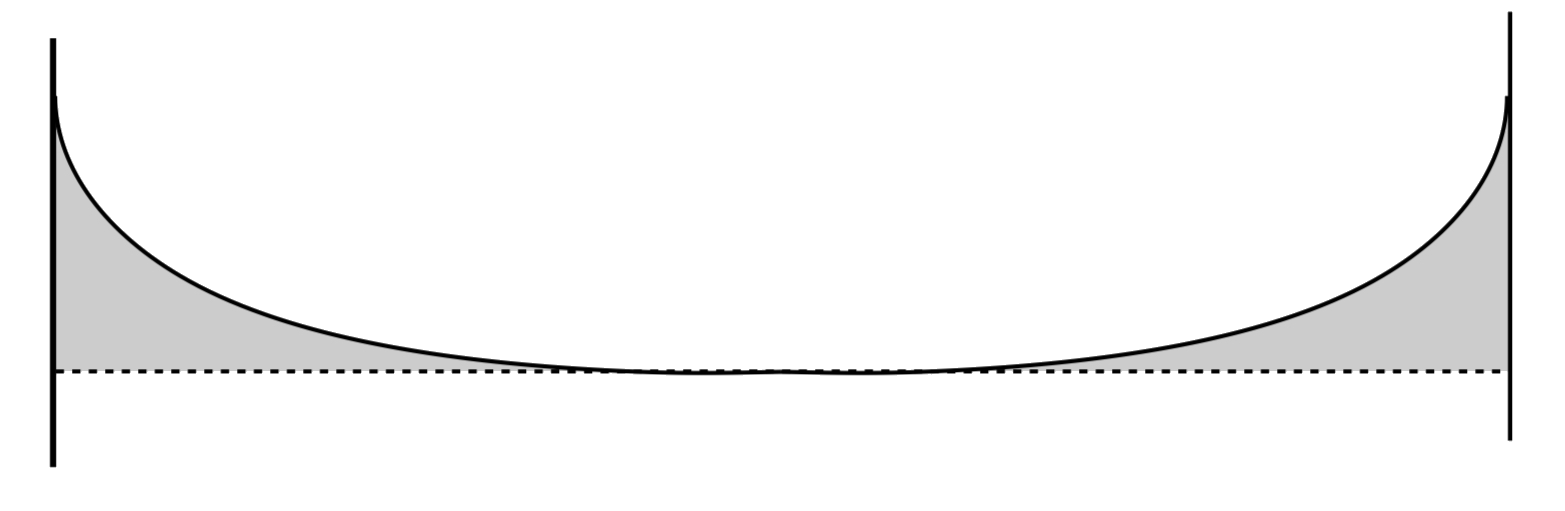
\includegraphics[width=8cm]{pr26.png}
\end{center}
By idea 17, the  gauge pressure due to capillary forces across a curved interface is $\rho gh = \frac{\sigma}{r}$ in cylindrical geometry where $H=V/(\pi r^2)$ gives the radius of the cylinder. We can determine the volume through a force balance:
$$\rho \Delta Vg=\sigma (2\pi r)$$
Plugging in our expression for $r$ gives:
$$\Delta V = \frac{2\sigma}{\rho g}\sqrt{\frac{V\pi}{H}} \approx 0.59 \text{ mL}$$
\blfootnote{It is believed that the symbolic answer to this problem in the handout is incorrect as it is not dimensionally correct.}
\end{solution}
\begin{solution}{normal}
Let us call $\xi$ a generalised coordinate if the entire state of a system can be described by this single number.\blfootnote{This problem is from the 1971 IPhO Problem 1. Refer to \url{https://www.jyu.fi/tdk/kastdk/olympiads/problems.html\#71prob} for a solution without lagrangian formalism.} Say we need to find the acceleration $\ddot\xi$ of coordinate $\xi$. If we can express the potential energy $\Pi$ of the system as a function $\Pi\left(\xi\right)$ of $\xi$ and the kinetic energy in the form $K=\mathcal{M}\dot\xi^2/2$ where coefficient $\mathcal{M}$ is a combination of masses of the bodies (and perhaps of moments of inertia), then
\[\ddot\xi=-\Pi'\left(\xi\right)/\mathcal{M}.\]Let us take the wedge's displacement as the coordinate $\xi$; if the displacement of the block along the surface of the wedge is $\eta$, then the center of mass from rest is
\[\eta(m_1\cos\alpha_1+m_2\cos\alpha_2)=(M+m_1+m_2)\xi.\]We then find that
\[\eta=\frac{(M+m_1+m_2)\xi}{(m_1\cos\alpha_1+m_2\cos\alpha_2)}\]We note that if we substitute this expression everywhere, we will get an extremely contrived answer. Thus, let us substitute this expressions with more sightful variable. Let
\[\varrho\equiv\frac{M+m_1+m_2}{m_1\cos\alpha_1+m_2\cos\alpha_2}.\]The potential energy as a function of $\xi$ is given by
\[\Pi \left(\xi\right)=m_1 g\eta\sin\alpha_1-m_2 g\eta\sin\alpha_2\]It is given that $\ddot{\xi}=\frac{\Pi' \left(\xi\right)}{\mathcal{M}}$. Thus by differentiating $\Pi\left(\xi\right)$ we get
\[\Pi\left(\xi\right)= \varrho(m_1\sin\alpha_1-m_2\sin\alpha_2).\]Finding $\mathcal{M}$ will be a bit harder. The kinetic energy of the block is given as the sum of the horizontal and vertical energies or
\begin{align*}
K&=\frac{1}{2}M\dot{\xi}^2+\frac{1}{2}m_1(\dot{\xi}-\dot{\eta}\cos\alpha_1)^2+\frac{1}{2}m_1(\dot{\eta}\sin\alpha_1)^2+\frac{1}{2}m_2(\dot{\xi}-\dot{\eta}\cos\alpha_2)^2+\frac{1}{2}m_2(\dot{\eta}\sin\alpha_2)^2\\
&=\frac{1}{2}M\dot{\xi}^2+\frac{1}{2}m_2(\dot{\xi}^2-2\dot\eta\dot\xi\cos\alpha_2+\dot\eta^2)+ \frac{1}{2}m_1(\dot{xi}^2-2\dot\eta\dot\xi\cos\alpha_1+\dot\eta^2)
\end{align*}We have that $\eta=\varrho\xi\implies\dot\eta=\varrho\dot\xi$. Thus, by substituting this into our expression for kinetic energy we have
\begin{align*}
K &=\frac{1}{2}M\dot{\xi}^2+\frac{1}{2}m_2(\dot{\xi}^2-2\dot\eta\dot\xi\cos\alpha_2+\varrho\dot\eta^2)+ \frac{1}{2}m_1(\dot{xi}^2-2\dot\eta\dot\xi\cos\alpha_1+\dot\eta^2) \\
&=\frac{1}{2}M\dot\xi^2+\frac{1}{2}m_2(\dot\xi^2-2\varrho\dot\xi^2\cos\alpha_2+\varrho\dot\xi^2) +\frac{1}{2}m_1(\dot\xi^2-2\varrho\dot\xi^2\cos\alpha_1+\varrho\dot\xi^2)\\
\mathcal{M}&=M+m_2(1-2\varrho\cos\alpha_2+\varrho^2)+m_1(1-2\varrho\cos\alpha_1+\varrho^2)
\end{align*}Now we apply our Lagrangian Formalism Identity,
\begin{align*}
&\ddot\xi=\frac{\Pi'\left(\xi\right)}{\mathcal{M}}=\dfrac{\varrho(m_1\sin\alpha_1-m_2\sin\alpha_2)}{M+m_2(1-2\varrho\cos\alpha_2+\varrho^2)+m_1(1-2\varrho\cos\alpha_1+\varrho^2)}\\
&=\dfrac{\varrho(m_1\sin\alpha_1-m_2\sin\alpha_2)}{(M+m_1+m_2)-2\varrho(m_1\cos\alpha_1+m_2\cos\alpha_2)+\varrho^2(m_1+m_2)}\\
&=\dfrac{\varrho(m_1\sin\alpha_1-m_2\sin\alpha_2)}{(M+m_1+m_2)-2\dfrac{M+m_1+m_2}{m_1\cos\alpha_1+m_2\cos\alpha_2}(m_1\cos\alpha_1+m_2\cos\alpha_2)+\varrho^2(m_1+m_2)}\\
&=\dfrac{\varrho(m_1\sin\alpha_1-m_2\sin\alpha_2)}{\varrho^2(m_1+m_2)-(M+m_1+m_2)}
=\dfrac{\dfrac{M+m_1+m_2}{m_1\cos\alpha_1+m_2\cos\alpha_2}(m_1\sin\alpha_1-m_2\sin\alpha_2)}{\left(\dfrac{M+m_1+m_2}{m_1\cos\alpha_1+m_2\cos\alpha_2}\right)^2(m_1+m_2)-(M+m_1+m_2)}\\
&=\dfrac{\left(\dfrac{M+m_1+m_2}{m_1\cos\alpha_1+m_2\cos\alpha_2}(m_1\sin\alpha_1-m_2\sin\alpha_2)\right)}{\left(\dfrac{(M+m_1+m_2)^2(m_1+m_2)-(M+m_1+m_2)(m_1\cos\alpha_1+m_2\cos\alpha_2)}{(m_1\cos\alpha_1+m_2\cos\alpha_2)^2}\right)}\\
&\boxed{a_0 = \frac{(m_1\cos\alpha_1 + m_2\cos\alpha_2)(m_1\sin\alpha_1 - m_2\sin\alpha_2)}{(m_1+m_2+M)(m_1+m_2) - (m_1\cos\alpha_1+m_2\cos\alpha_2)^2}}
\end{align*}
This is extremely long, yes, but to do well at the International Olympiad, you must be familiar and not scared to bash it all out.
\end{solution}

\begin{solution}{normal}
Consider a reference frame moving with speed $u$ opposite to the direction of the cars. \vspace{3mm}

Cars at the end will be moving with speed $v+u$, and the distance between them will be $v\tau$.\vspace{3mm}

Cars at the front will be moving at speed $u$ (because they are stopped) and have a distance $l$ between them.\vspace{3mm}

Now we take ratios of speed to length and equate them to get
\begin{align*}
\frac{v\tau}{v+u} &= \frac{l}{u}\\
v\tau u &= vl + ul \\
v\tau u - ul &= vl \implies u(v\tau - l) = vl\\
u &= \boxed{\frac{v}{v\tau/l -1}\approx 3.4\;\text{m/s}}
\end{align*}

\end{solution}
\begin{solution}{normal}
Consider the time when the angle between the line joining the edge to the rod makes an angle $\theta$, with the vertical. We want that the normal should always be positive (outwards).
The velocity of the rod at this time, $\nu$, can be calculated using energy conservation $\frac{1}{2} m \nu^2 = \frac{1}{2}mv^2 + mgR(1-\cos \theta)$.
Setting total forces along the line joining the rod to the edge to $0$, we get that
\begin{align*}
\frac{m\nu^2}{R} + N &= mg \cos \theta \\
N &= mg \cos \theta - \frac{2\cdot \dfrac{1}{2}m\nu^2}{R}\\
&= mg \cos \theta - \dfrac{mv^2 + 2mgR(1-\cos \theta)}{R} \\
0 &\le 3mg \cos \theta - \frac{mv^2 + 2mgR}{R} \\
\cos \theta &\ge\frac{1}{3}\left(2+\frac{v^2}{gR}\right)
\end{align*}
for all values of $\theta$ that can be achieved. The maximum value of $\theta$ will be alpha, so 
\[\cos \alpha\ge\frac{1}{3}\left(2+\frac{v^2}{gR}\right)
\] is a necessary and sufficient condition.
\end{solution}

\begin{solution}{normal}
From the first two collisions, we can deduce that all three bodies lie on the same plane. For simplicity, let this be the x-y plane.\vspace{3mm} 

Additionally, we can assume that all three bodies lie on the x-axis, with body $a$ at the origin $O$. We can then plot the motion of the bodies in three dimensions (with time as the third dimension) as follows:
\begin{center}
    \begin{asy}
        settings.render=0;
        import three;
        unitsize(6cm);
        currentprojection=perspective(0.5,-1.1,0.7);
        draw((0,0,0)--(1,1,1),blue);
        draw((0.5,0,0)--(2/3,1,1),green);
        draw((1,0,0)--(0,2/3,2/3),red);
        draw((0,0,0)--(1,0,0)--(1,1,0)--(0,1,0)--cycle);
        draw((0,0,0)--(1.2,0,0),arrow=Arrow3());
        draw((0,0,0)--(0,1.6,0),arrow=Arrow3());
        draw((0,0,0)--(0,0,1.2),arrow=Arrow3());
        draw((0,0,0)--(0,0,1));
        draw((0,1,0)--(0,1,1));
        draw((1,1,0)--(1,1,1));
        draw((1,0,0)--(1,0,1));
        draw((0,0,1)--(1,0,1)--(1,1,1)--(0,1,1)--cycle);
        label("$x$",(1.2,0,0),SE);
        label("$y$",(0,1.6,0),NE);
        label("$t$",(0,0,1.2),N);
        dot((0,0,0));
        dot((0.5,0,0));
        dot((1,0,0));
        dot((0.6,0.6,0.6));
        dot((0.4,0.4,0.4));
        dot((0.55,0.3,0.3));
        label("$A$",(0,0,0),SW);
        label("$B$",(0.5,0,0),SW);
        label("$C$",(1,0,0),SW);
    \end{asy}
\end{center}

Since body $a$ collides with body $b$, both the trajectories of $a$ and $b$ must lie on some unique plane $\mathcal{P}$ in our 3-D plot.\vspace{3mm}

Since body $a$ collides with body $b$, both the trajectories of $a$ and $c$ must lie on some unique plane $\mathcal{P'}$ in our 3-D plot.\vspace{3mm}

However, both $\mathcal{P}$ and $\mathcal{P'}$ contain the trajectory of $A$ and the x-axis, so they must be the same plane.\vspace{3mm}

Therefore, $\boxed{\text{yes}}$, $b$ and $c$ would collide if $a$ is missing.
\end{solution}
\begin{solution}{hard}
Since the potential energy in a sphere is lower, let us assume that the potential energy stored in the surface is going to completely transferred to kinetic energy instantaneously. Let us determine the radius of this sphere. Since the volume is equal, we have:
$$\pi(d/2)^2 h = \frac{4}{3}\pi r^3 \implies r = \frac{1}{2}\left(\frac{3d^2h}{2}\right)^{1/3}$$
Therefore, the change in energy is:
$$\sigma\Delta S = \sigma\pi dh - \sigma4\pi \left(\frac{1}{2}\left(\frac{3d^2h}{2}\right)^{1/3}\right)^2 = \sigma\pi h\sqrt[3]h\left(\sqrt[3]h-\sqrt[3]{9d/4}\right)$$
Let us assume this change in energy causes half of the liquid to move at a speed of $v$. Then:
$$\frac{1}{2}(0.5 m)v^2 = \sigma\pi h\sqrt[3]h\left(\sqrt[3]h-\sqrt[3]{9d/4}\right) \implies
v = 4\sqrt{\frac{\sigma}{\rho d}}\sqrt{\frac{\sqrt[3]h-\sqrt[3]{9d/4}}{\sqrt[3]h}}
$$
using the fact that $m=\rho \pi (d/2)^2h$. If we take $v$ to be the average velocity, then the characteristic time would be given by:
$$t=\frac{h}{v}=\frac{1}{4}\sqrt{\frac{\rho d}{\sigma}}\sqrt{\frac{\sqrt[3]{h^7}}{\sqrt[3]h-\sqrt[3]{9d/4}}}$$
We see that the characteristic time depends on the height $h$ of the original cylinder. Since we want the time for the most unstable perturbations, we want to maximize $t$ and we can do this by taking the derivative. Doing so gives us:
$$h=\left(\frac{7}{6}\right)^3\frac{9}{4}d\approx 3.57d$$
Therefore, the characteristic time is:
$$t=\frac{1}{4}\sqrt{\frac{\rho d}{\sigma}}\sqrt{\frac{\sqrt[3]{(3.57d)^7}}{\sqrt[3]{3.57d}-\sqrt[3]{9d/4}}} \approx 0.0088 \text{ s}$$
\tcbline 
\textbf{Solution 2.} Dimensional analysis tells us that the characteristic time is:
$$t =\sqrt \frac{\rho d^3}{\sigma}=0.003727 \text{ s}$$
\end{solution}
\begin{solution}{hard}
When the pulley is let go, one side of the rope will go up a distance $\xi$ while the other side will go down a distance $\xi$. The change in potential energy of this is the categorized as 
\[\Pi(\xi) = -\rho g(L - 2l - \pi R)\xi \implies -\Pi'(\xi) = \rho g(L - 2l - \pi R)\]
The kinetic energy of the system will then be 
\[K = \frac{1}{2}m\dot\xi^2 + \frac{1}{2}\rho L\dot\xi^2\]
This implies that the effective mass, $\mathcal{M}$, is $\mathcal{M} = m + \rho L$. We then get the acceleration of the system to be 
\[a \equiv \frac{\rho g(L - 2l - \pi R)}{m + \rho L}\]
Now, we write for the displacement of parts of the system times their mass divided by the total effective mass of the system $\mathcal{M}$. Differentiating that with respect to $\xi$ will give us our accelerations in the $x$ and $y$ direction. In the $x$ direction, we have
\begin{align*}
x &= \frac{2R\xi\rho}{m + \rho L}\\
a_x &= \frac{2R\rho a}{m + \rho L}
\end{align*}
In the $y$ direction, we have 
\begin{align*}
y &= \frac{(L - 2l -\pi R)\rho\xi}{m + \rho L}\\
a_y &= \frac{(L - 2l - \pi R)\rho a}{m + \rho L}
\end{align*}
By $F=ma$, we have the direction of force in the $x$ and $y$ direction to then be 
\[\boxed{F_x = 2R\rho a}\]
\begin{align*}
F_y - (m+\rho L)g = -\rho a (L - \pi R - 2l)\\
\boxed{\therefore F_y = -\rho a(L-\pi R - 2l) + (m + \rho L)g}
\end{align*}
\end{solution}

\begin{solution}{normal}
Assuming that idea 2 is correct, it may be proved that between the quantity of heat $Q$, which in a cyclical process-of the kind described above is transformed into work (or, where the process is in the reverse order, generated by work), and the quantity of heat $Q_2$ which is transferred at the same time from a hotter to a colder body Cor vice versa), there exists a relation independent of the nature of the variable body which acts as the medium of the transformation and transfer; and thus that, if several cyclical processes are performed, with the same reservoirs of heat $K_1$ and $K_2$ , but with different variable bodies, the ratio 3. will be the same for all. If we suppose the processes so arranged, according to their magnitude, that the quantity of heat $Q$, which is transformed into work, has in all of them a constant value, then we have only to consider the magnitude of the quantity of heat $Q_2$. which is transferred, and the principle which is to be proved takes the following form: 
\vspace{3mm}

If where two different variable bodies are used, the quantity of heat $Q$ transformed into work is the same, then the quantity of heat $Q_2$ which is transferred, will also be the same.
\vspace{3mm}

Let there, if possible, be two bodies $\text{A}$ and $\text{A}'$ (e.g. the perfect gas and the combined mass of liquid and vapour, described above) for which the values of $Q$ are equal, but those of the transferred quantities of heat are different, and let these different values be called $Q_2$, and $Q'_2$, respectively: $Q_2'$, being the greater of the two. Now let us in the first place subject the body a to a cyclical process, such that the quantity of heat $Q$ is transformed into work, and the quantity $Q$ is transferred from $K_2$ to $K_1$. Next let us subject $\text{A}'$ to a cyclical process of the reverse description, so that the quantity of heat $Q$ is generated out of work, and the quantity $Q_2'$. is transferred from $K_2$ to $K_1$. Then the above two changes, from heat into work, and work into heat, will cancel each other since we may suppose that when in the first process the heat $Q$ has been taken from the body $K_1$ and transformed into work, this same work is expended in the second process in producing the heat $Q$, which is then returned to the same body $K_1$. In all other respects also the bodies will have returned, at the end of the two operations, to their original condition, with one exception only. The quantity of heat $Q_2'$ transferred from $K_1$, to $K_2$ has been assumed to be greater than the quantity $Q_2$ transferred from $K_1$ to $K_2$. Hence, these two do not cancel each other, but there remains at the end a quantity of heat, represented by the difference $\Delta Q_2$, which has passed over from $K_1$ to $K_2$. Hence a passage of heat will have taken place from a colder to a warmer body without any other compensating change. But this contradicts the fundamental principle. Hence the assumption that $Q_2'$ is greater than $Q_2$, must be false. 
\vspace{3mm}

Again, if we make the opposite assumption, that $Q_2'$, is less than $Q_2$ we may suppose the body $\text{A}'$ to undergo the cyclical process in the first, and a in the reverse direction. We then arrive similarly at the result that a quantity of heat $Q_2- Q_2'$, has passed from the colder body $K_2$ to the hotter $K_1$ which is again contrary to the principle.
\vspace{3mm}

Since then $Q_2'$, can be neitlier greater nor less than $Q_2$, it must be equal to $Q_2$; which was to be proved. We will now give to the result thus obtained the mathematical form most convenient for our subsequent reasoning. Since the quotient $Q/Q_2$ is independent of the nature of the variable body (fact 2), it can only depend on the temperature of the two bodies $K_1$ and $K_2$ which act as heat reservoirs. The same will of course be true of the sum
\[1 + \frac{Q}{Q_2} = \frac{Q + Q_2}{Q_2} = \frac{Q_1}{Q_2}.\]
This last ratio, which is that between the whole heat received and the heat transferred, we shall select for further consideration; and shall express the result obtained in this section as follows: \vspace{3mm}

The ratio $Q_1/Q_2$ can only depend on the temperatures $T_1$ and $T_2$.
\vspace{3mm}

This leads to the equation:
\[\frac{Q_1}{Q_2} = f(T_1, T_2).\]
Since the process is isothermal, we can obtain the equation
\[\frac{Q_1}{Q_2} = \dfrac{nRT_1\ln \frac{V_f}{V_i}}{nRT_2 \ln \frac{V_f}{V_1}} = \frac{T_1}{T_2}.\]
Using this definition, the Carnot's Cycle efficiency can then be rewritten as 
\[\eta_C = 1 - \frac{Q_2}{Q_1} = 1 - \frac{T_2}{T_1}.\]
$\square$
\blfootnote{Part of this solution is taken from Rudolf Clausius' original work "The Mechanical Theory of Heat".}
\end{solution}
\begin{solution}{normal}
Let the friction force directed on the block to the right be $f_1$, the friction force directed on to the block on the left be $f_2$, and let the tension directed from the string be $T$. Drawing a freebody diagram results in 4 equations. (The two small blocks have the same accelerations because they are connected by the same string).
\begin{align}
F - f_1 &= Ma_1\\
f_1 - T &= ma_2\\
f_2 &= Ma_3\\
T - f_2 &= ma_2
\end{align}
We consider four options: all the bodies move together, the rightmost block moves separately, all three components move separately, or the left block moves separately.
\vspace{2mm}

\textbf{Case 1:} (all the bodies move together, $a_1 = a_2 = a_3$)
\vspace{2mm}

Since all the bodies move together, then they move at the same acceleration. This means that our equations are now
\begin{align}
F - f_1 &= Ma\\
f_1 - T &= ma\\
f_2 &= Ma\\
T - f_2 &= ma
\end{align}
Substituting equation (3) into equation (4) gives us 
\begin{align*}
T - Ma &= ma\\
T = (m + M)a
\end{align*}
Substituting our result for tension into equation (2) gives us 
\begin{align*}
f_1 - (m + M)a &= ma\\
f_1 = (2m + M)a
\end{align*}
Taking this result and now substituting into equation (1) gives us 
\begin{align*}
F - (2m + M)a = Ma\\
F = 2(m + M)a\\
\boxed{a = \frac{F}{2(m + M)}}
\end{align*}
From equation (1), we note that 
\[F - Ma = f_1 \leq\mu mg\]
Plugging in our equation for acceleration gives us 
\begin{align*}
F - M \frac{F}{2(m + M)} \leq \mu mg\\
F\left(1 - \frac{1}{2(m + M)}\right) \leq \mu mg\\
F\left(\frac{M + 2m}{2(m + M)}\right) \leq \mu mg\\
\boxed{F \leq 2\mu mg \frac{m +M}{m + 2M}}
\end{align*}

\textbf{Case 2:} (The rightmost block moves separately, $a_2 = a_3$, $f_2 = \mu mg$)
\vspace{2mm}

In this case, we have our equations to be 
\begin{align}
F - \mu mg &= Ma_1\\
\mu mg - T &= ma_2\\
f_2 &= Ma_2\\
T - f_2 &= ma_2
\end{align}
From this, we find that 
\begin{align*}
\boxed{a_1 = \frac{F - \mu mg}{M}}\\
\boxed{a_2 = \frac{\mu mg}{M + 2m}}
\end{align*}
For the block to move, we must have 
\begin{align*}
Ma_2 \leq \mu mg\\
\frac{\mu mMg}{M + 2m} \leq \mu mg\\
\frac{M}{M + 2m} \leq 1
\end{align*}
This works, since both the denominator is greater than the numerator. Thus, we can continue with our calculations and find that from case 1, we have that if the force is 
\[F \leq 2\mu mg \frac{m +M}{m + 2M}\]
then our acceleration would be
\[\boxed{a = \frac{F}{2(m + M)}}\]
if the force does not satisfy that constraint, then we have the accelerations to be the results we found before. 
\vspace{2mm}

\textbf{Case 3:} (all three components move separately, $a_1 \neq a_2 \neq a_3$)
\vspace{2mm}

If $a_1\neq a_2 \neq a_3$, then that implies that the $f_1 = \mu mg$ and $f_2 = \mu mg$. Looking at our systems of equations 
\begin{align}
F - f_1 &= Ma_1\\
f_1 - T &= ma_2\\
f_2 &= Ma_3\\
T - f_2 &= ma_2
\end{align}
We find that $a_2 = 0$ which is impossible.
\vspace{2mm}

\textbf{Case 4:} (the left block moves separately, $a_1 = a_2$, $f_2 = \mu mg$)
Our systems of equation would then be 
\begin{align}
F - f_1 &= Ma_1\\
f_1 - T &= ma_1\\
\mu mg &= Ma_3\\
T - \mu mg &= ma_1
\end{align}
Solving these equations gives us 
\[a_1 = \frac{F - \mu mg}{M + 2m}\]
Substituting back into equation (1) gives us 
\begin{align*}
F - f_1 = M\frac{F - \mu mg}{M + 2m}\\
F - M\frac{F - \mu mg}{M + 2m} \leq \mu mg
\end{align*}
Multiplying across gives us
\[(M + 2m)F - M(F -\mu mg) \leq \mu mg (M + 2m)\]
Solving this inequality gives us
\[F \leq \mu mg\]
which is impossible because that would then imply that $a_1 \leq 0$.
\end{solution}

\begin{solution}{normal}
\begin{center}
    \begin{asy}
/* Geogebra to Asymptote conversion, documentation at artofproblemsolving.com/Wiki go to User:Azjps/geogebra */
import graph; usepackage("amsmath"); size(12cm);
real labelscalefactor = 0.5; /* changes label-to-point distance */
pen dps = linewidth(0.7) + fontsize(10); defaultpen(dps); /* default pen style */
pen dotstyle = black; /* point style */
real xmin = -0.8860362915535339, xmax = 10.195219297936417, ymin = -0.028752442281231375, ymax = 7.618229720713907; /* image dimensions */

/* draw figures */
draw((3,5)--(9,5));
draw((3,2)--(9,2));
draw((6,2)--(5,4),EndArrow(6));
draw((6,4)--(5,4),EndArrow(6));
draw((6,2)--(6,4),EndArrow(6));
label("$v$",(5.169732517165664,3.056702469065482),SE*labelscalefactor);
label("$v\sin\varphi$",(5.204075251430613,4.350278793045199),SE*labelscalefactor);
label("$v\cos\varphi$",(6.028300873789369,3.216968562301907),SE*labelscalefactor);
draw(shift((6,2))*xscale(0.48971473714830527)*yscale(0.48971473714830527)*arc((0,0),1,90,116.56505117707799));
label("$\varphi$",(5.730663843493152,2.7590654387692643),SE*labelscalefactor);
/* dots and labels */
clip((xmin,ymin)--(xmin,ymax)--(xmax,ymax)--(xmax,ymin)--cycle);
/* end of picture */
    \end{asy}
\end{center}
Since we have $u>v>v\sin{\varphi} \ \forall  \ 90^\circ > \varphi \geq 0^\circ$, this means that the fast-flowing river carries the boy a lateral distance of $a = (u-v\sin{\varphi})T$ (where $T$ is the time it takes to reach the other shore) from point B. \vspace{3mm}

Since the time taken to cross the river is simply $T = \dfrac{L}{v\cos{\varphi}}$, this means that $$a = \frac{(u-v\sin{\varphi})L}{v\cos{\varphi}} = \frac{(2-\sin{\varphi})L}{\cos{\varphi}}$$ where the last expression is achieved by substituting the given values.\vspace{3mm}

Now, for minimising $a$, we have $$\frac{\text{d}a}{\text{d}\varphi} =  L\frac{\text{d}}{\text{d}\varphi}\left(\frac{2-\sin{\varphi}}{\cos{\varphi}}\right) = \frac{L(2\sin{\varphi} - 1)}{\cos^2{\varphi}}$$ which clearly vanishes at $\sin{\varphi} = \frac{1}{2}$ or $\varphi = 30^\circ$.\vspace{3mm}

Substituting this in the expression for $a$, we have $$a_{\text{min}} = \frac{L(2- \frac{1}{2})}{\sqrt{3}/2} = \boxed{L\sqrt{3}}$$ 
\tcbline 
\newpage
\textbf{Solution 2:} Let the velocity of the boy with respect to the ground be $\vec{w}=\vec{u}+\vec{v}$. Since $\vec{u}$, the velocity of the water is fixed and the magnitude of $\vec{v}$ is fixed, we can only change the orientation.
\begin{center}
    \begin{asy}
    import graph; size(10cm); 
real labelscalefactor = 0.5; /* changes label-to-point distance */
pen dps = linewidth(0.7) + fontsize(10); defaultpen(dps); /* default pen style */ 
pen dotstyle = black; /* point style */ 
real xmin = -10.194991692355861, xmax = 9.869014624902043, ymin = -4.997678398452476, ymax = 4.799658019623726;  /* image dimensions */
pen xfqqff = rgb(0.4980392156862745,0,1); 
 /* draw figures */
draw(circle((0,0), 3),  linetype("2 2")); 
draw((-6,0)--(0,0),  red,EndArrow(6)); 
draw((0,0)--(-1.3956412397187756,2.6555951366871113),  blue,EndArrow(6)); 
draw((0,0)--(0,3),  blue,EndArrow(6)); 
draw((0,0)--(-2.583184425515349,1.5255026134933156),  blue,EndArrow(6)); 
draw((0,0)--(1.3176303960148275,2.695153082757603),  blue,EndArrow(6)); 
draw((0,0)--(2.640750554328599,1.423529595692761),  blue,EndArrow(6)); 
draw((0,0)--(3,0),  blue,EndArrow(6)); 
draw((0,0)--(2.6955138280127677,-1.3168922518535657),  blue,EndArrow(6)); 
draw((0,0)--(1.5864742001929164,-2.5461931608034467),  blue,EndArrow(6)); 
draw((0,0)--(0,-3),  blue,EndArrow(6)); 
draw((0,0)--(-1.373869769022932,-2.666923669279808),  blue,EndArrow(6)); 
draw((0,0)--(-2.5898903823572463,-1.514089761993468),  blue,EndArrow(6)); 
draw((-6,0)--(-1.3956412397187759,2.6555951366871113),  xfqqff,EndArrow(6)); 
label("$v$",(-0.7643220563932647,1.7543237904219548),SE*labelscalefactor,blue); 
label("$u$",(-3.3456562024732293,-0.17965656499198404),SE*labelscalefactor,red); 
label("$w$",(-4.108323109269582,1.7103237765683192),SE*labelscalefactor,xfqqff); 
draw(shift((-6,0))*xscale(0.5863431464058904)*yscale(0.5863431464058904)*arc((0,0),1,0,29.974490165312012)); 
label("$\theta$",(-5.3696568397404745,0.2943233748128856),SE*labelscalefactor); 
 /* dots and labels */
clip((xmin,ymin)--(xmin,ymax)--(xmax,ymax)--(xmax,ymin)--cycle); 
 /* end of picture */
 \end{asy}
\end{center}
The superposition of all possible orientations fill up a circle as shown. We want the velocity relative to the ground to make as large an angle as possible. To achieve this, $w$, $u$, and $v$ must be the three sides of a right angled triangle such that:
$$w^2=u^2-v^2 \implies w = \sqrt{3} \text{ m/s}$$
The time to cross is given by:
$$t=\frac{L}{w\sin\theta}$$
and the horizontal distance traveled during this time is:
$$a=w\cos\theta t = \frac{L}{\tan\theta} = \boxed{L\sqrt{3}}$$
\end{solution}
\begin{solution}{normal}
\textbf{a)}  Denote the first ball with a final speed $v_1$ and the other two balls with final speed $v_2$.
\begin{center}
\begin{asy}
size(6cm);
defaultpen(fontsize(10pt));

real circledist = 6;
draw(shift(-circledist, 0)*unitcircle);
draw("$v$", (-circledist + 1, 0)--(-circledist + 4, 0), dir(90), Arrow(TeXHead), Margins);

draw(unitcircle, dashed);
draw(shift(2*dir(45))*unitcircle);
draw(shift(2*dir(-45))*unitcircle);

real eps = 0.3, eps2 = 0.7;
draw((3+eps)*dir(45) -- 5*dir(45), Arrow(TeXHead));
draw((3+eps)*dir(45) -- ((3+eps)*dir(45) + sqrt(2)*dir(0)), dashed);
draw((3+eps)*dir(-45) -- 5*dir(-45), Arrow(TeXHead));
draw((3+eps)*dir(-45) -- ((3+eps)*dir(-45) + sqrt(2)*dir(0)), dashed);
draw("$30^\circ$", arc((3+eps)*dir(45), eps2, 0, 45), dir(22.5));
draw("$30^\circ$", arc((3+eps)*dir(-45), eps2, 0, -45), dir(-22.5));
\end{asy}
\end{center}
In this problem, we're given an elastic collision, so we know that both momentum and energy are conserved. Conservation of momentum gives
\[
    v_1 + \frac{\sqrt{3}}{2} v_2 + \frac{\sqrt{3}}{2} v_2 = v
    \implies v_1 + \sqrt 3 v_2 = v,
\]and conservation of energy gives
\[
    2\left(\frac{1}{2} m v_2^2\right) + \frac{1}{2} m v_1^2 = \frac{1}{2} m v^2
    \implies 2 v_2^2 + v_1^2 = v^2.
\]
This gives us two equations. Our goal is to find $v_1$, thus we first rearrange our conservation of momentum equation to get $v_2$ in terms of $v_1$ and then substitute back in to get $v_1$.
\[
v_1=v-\sqrt 3v_2
\]putting this in to our conservation of energy equation gives us
\[
2(v - \sqrt 3v_2)^2 + v_1^2 = v^2.
\]Expanding this equation out gives us
\[
2v_2^2 + 3v_2^2 - 2\sqrt 3v_2v + v^2 = v^2
\]
Taking out $v^2$ from both sides, and then dividing by $v_2$ on both sides gets us the equation
\[2v_2 + 3v_2 -2\sqrt 3v = 0\implies 5v_2 = 2\sqrt 3v\implies v_2 = \frac{2\sqrt 3}{5}v
\]Substituting $v_2$ back into our conservation of momentum equation gives us 
\[v_1 = v - \sqrt 3\frac{2\sqrt 3}{5}v\implies\boxed{|v_1| = \frac{1}{5}v.}
\]
\textbf{b)} Suppose the moving ball first strikes the lower ball. Let the x-direction point in the line joining their centers. Therefore, $v_{1,x}= v\cos30^\circ$ and the perpendicular component of velocity is $v_{1,y} = v\sin30^\circ$. Note that the impulse acts along line joining their center, therefore the perpendicular component of its velocity is unchanged. Conservation of momentum gives:
$$v_{1,x}=v_1'+v_2'$$Conservation of energy:
$$v_{1,x}^2+v_{1,y}^2=v_1'^2+v_{1,y}^2+v_2'^2 \implies v_{1,x}^2=v_1'^2+v_2'^2$$Notice that in the x-direction, this gives the same behavior as a head-on collision between two identical balls. Therefore, the velocity of the moving ball becomes zero along the x-direction. Now the moving ball will strike the upper ball with a speed $v\cos30^\circ$.

This second collision is identical to the first. The component of velocity along the line joining their centers is $(v\cos 30^\circ)\sin 30^\circ$ and the component of velocity perpendicular to this line is $(v\cos 30^\circ)\sin 30^\circ$. Again, only the component of velocity perpendicular to this line will survive at the end so the final answer is:
$$\boxed{v_f=v\sin^230^\circ=\frac{v}{4}}$$
\end{solution}

\begin{solution}{normal}
First, let us convert the temperatures from celsius to kelvin.
\begin{align*}
T_1 &= 20 + 273 = 293\;\mathrm{K}\\\
T_2 &= 0 + 273 = 273\;\mathrm{K}
\end{align*}Furthermore, converting the time from hours to seconds gives us $t = 36000\;\mathrm{s}$
Note that the heat flux as given in Kalda’s introduction to thermoelectricity is
\[\Phi = \frac{P}{\eta_C}\]
where $\eta_C = 1 - \frac{T_c}{T_h}$. For a small increment of time $dt$ the mass gained is $dm$ and therefore the heat flux is $\frac{dm}{dt}\lambda$. Equating these two expressions together gives us 
\[\frac{dm}{dt}\lambda = I^2 R\frac{T_h}{T_h - T_c}\implies \int_{0}^{m} dm = \int_{0}^{t} I^2 R \frac{T_h}{T_h - T_c}.\]
Integrating through and dividing both sides by $\lambda$ tells us that 
\[m = \boxed{\frac{I^2 R tT_h}{(T_h - T_c)\lambda}\approx 1.5\;\mathrm{g}}.\]
\end{solution}
\begin{solution}{normal}
Heat leaving the room in stable state is equal to heat produced by heater by Fourier's law.
$$P(T_2) = k(T_2-T_1)$$
In the second case,
$$ P(T_4) = k(T_4-T_3)$$
Therefore, point $(T_4,P(T_4))$ must be on the line which passes through point $(T_3,0)$ with the same slope as the line passing through $(T_2,P(T_2))$ and $(T_1,0)$
This gives $\boxed {T_4=1.4T_3}$
\begin{center}
    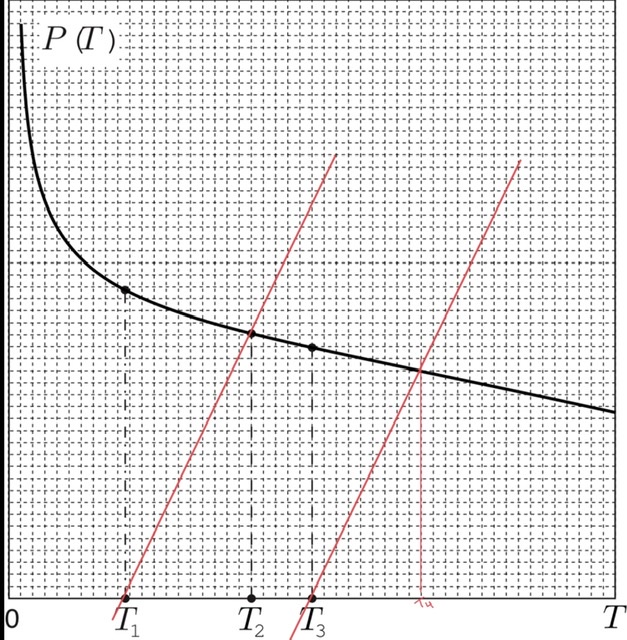
\includegraphics[width=8cm]{t38.jpeg}
\end{center}
\end{solution}
\begin{solution}{normal}
At nominal voltage, we have two relations of $P=I_0 V_0$ and $R=\frac{V_0}{I_0}$. As resistivity is proportional to temperature, we then have the temperature at which the filament is supposed to emit light to be  
\[\frac{R}{R_0} = \frac{T}{T_0}\implies T = \frac{RT_0}{R_0} = \boxed{\frac{V_0}{I_0 R_0}T_0}.\]
The power $P$ radiated according to Stefan-Boltzmann law is 
\[\frac{P}{A} = k\sigma T^4\implies P = k \sigma T^4\cdot \pi ld\implies ld = \frac{V_0I_0}{\pi k \sigma T^4}.\]
The initial resistance is given by 
\[R = \frac{\rho_0 l}{A} = \frac{\rho_0 l}{\pi d^2/4}\implies l = \boxed{\frac{\pi R_0 d^2}{4\rho_0}}.\]
Therefore, 
\[\frac{\pi R_0}{4\rho_0} d^3 = \frac{V_0I_0}{\pi k \sigma T^4}\implies d = \boxed{\sqrt[3]{\frac{4V_0I_0\rho_0}{k\pi^2 R_0 \sigma T^4}}}.\]
\end{solution}
\begin{solution}{normal}
The key difference between the barrels is that the walls in barrel provide a non-zero momentum to every small elemental mass that exits through the tap, while the other does not. Some non-zero work is done by the force exerted by these walls on the water molecules, which is not true for the other . So we first write the conservation of energy equation for the barrel: Let the small $dm$ mass of water element exit at a velocity $v_1$ from the tap of the barrel,$$\frac{1}{2} dm {v_1}^2 = dm g H$$and by impulse momentum theorem,$$F_{\text{walls}} = dm v_2 \implies (\rho g A_0 H)dt = (\rho A_0 v_2 dt) v_2$$From these two equations, we have the answers $\boxed{\sqrt{2gH}}$ and $\boxed{\sqrt{gH}}$.
\end{solution}

\begin{solution}{normal}
The rope will intuitively be something like a spiral.\vspace{3mm} 

Since the rope can go up to infinity, let's consider the last point instead. We set the point where all the shockwaves coincide at the origin and we use polar coordinates since we are going to be dealing with distances.\vspace{3mm}

The rope lies along the curve $r(\theta)$, where $r(0)$ is the last point to be ignited. It takes time $r(0)/c$ for the shockwave from the last ignition point to reach the origin. If we go back an angle $d\theta$ along the rope, then it takes time $$\dfrac{r(d\theta)}{c}-\dfrac{ds}{v}$$
for that shockwave to reach the origin, where $ds$ is the infinitesimal arc length. Note that \[ds=\sqrt{r^2d\theta^2+dr^2}.\] 

We can set up our differential equation from this knowledge. For each $r(\theta)$, we want \[\dfrac{r(\theta+d\theta)-r(\theta)}{c}=\dfrac{ds}{v}\]

Divide both sides by $d\theta$ to get \[r'/c=\sqrt{r^2+r'^2}/v\]

Square both sides to get \[\dfrac{r'^2}{c^2}=\dfrac{r^2}{v^2}+\dfrac{r'^2}{v^2}\]

Combining like terms and simplifying gives us \[\frac{dr}{d\theta}=r\sqrt{\frac{c^2}{v^2-c^2}}\]

This is a separable differential equation which gives us solution \[r=\boxed{Ce^{\sqrt{\dfrac{c^2}{v^2-c^2}}\theta}}\]
\end{solution}
\begin{solution}{normal}
The velocity of the blob just when the blob is about to hit the surface is found by conservation of mechanical energy$$\frac{1}{2} m v^2 = mgh \implies v= \sqrt{2gh}$$The Impulse (change in momentum) imparted perpendicular to the blob is clearly$$\Delta{p_{\perp}} = m\sqrt{2gh}$$From idea 60,$${\Delta{p_{\perp}}} = \int{\mu Ndt} =  \mu{\Delta{p_{\parallel}}}  \implies \Delta{p_{\perp}} = \mu m\sqrt{2gh}$$Hence$$\boxed{v = u - \mu \sqrt{2gh}}$$
\end{solution}

\begin{solution}{normal}
Let us observe what happens to the work done at small changes of $da$ and $dh$.
\begin{center}
\begin{asy}
size(5cm);
draw((0,0)--(-4/3, 0), blue);
draw((0,1)--(-4/3, 0), blue);
draw((0,0)--(0, 1), blue);

dot((0,0), red);
dot((0,1), red);
dot((-4/3,0), red);
pair A,B, C;
B = (0,0);
A = (0,1);
C = (-4/3,0);

label("$da$", (-1/2,0), S);
label("$dl$", (-5/6,3/4), 2S);
label("$dh$", (0,1/2), 1E);
draw(anglemark(B, C, A ,4));
label("$\phi$",C+0.2, NE);
\end{asy}
\end{center}

The work due to friction will be
\[W_f=\mu mg\cos\phi dl\]Since $dl\cos\phi=da$ then
\[W_f=\mu mg da\]Integrating all of these small work variables from 0 to $a$ gives us the work produced by friction as
\[W_f=\mu mga\]The work produced by gravity is $mgh$ thus the total work $W_{\text{tot}}$ is
\[W_{\text{tot}}=mgh+\mu mga=\boxed{mg(h+\mu a)}\]
\end{solution}

\begin{solution}{normal}
The tire does not exchange any heat with its surroundings which means that it undergoes an adiabatic expansion/compression. Since we are relating two state variables $p$ and $T$, we use the relation
\[p^{1 - \gamma}T^{\gamma} = \text{const.}\]Substituting both final and initial variables shows us
\[p_0^{1 - \gamma} T_0^{\gamma} = p_f^{1 - \gamma} T_f^{\gamma}\implies T_f = T_0 \left(\frac{p_f}{p_0}\right)^{\frac{\gamma - 1}{\gamma}} = T_0 \left(\frac{p_0 + p_1}{p_0}\right)^{\frac{\gamma - 1}{\gamma}} = 3^{\frac{\gamma - 1}{\gamma}} T_0\approx 400\;\mathrm{K}.\]
\end{solution}
\begin{solution}{normal}
\textbf{a)} The angular momentum of the rod about the end of it's axis before the collision is defined by
\[L_0=Mvl-\frac{1}{3}Ml^2\omega.\]
After the rod collides with the post it's angular momentum right after impact is 
\[L_a=Mv'l-\frac{1}{3}Ml^2\omega'.\]
Since angular momentum is conserved in the entire process we have
\[L_0=L_a\implies Mvl-\frac{1}{3}Ml^2\omega=Mv'l-\frac{1}{3}Ml^2\omega'\implies v-\frac{1}{3}\omega l=v'-\frac{1}{3}\omega' l.\]
We know that the condition for the rod being at the end, is the relation 
\[
v' + l\omega' = 0\implies \omega' = -\frac{v'}{l}
\]Substituting our relation of $\omega'$ and $v'$ into our simplified angular momentum equation gives us
\begin{align*}
v-\frac{1}{3}\omega l = \frac{4}{3}v'\\
\boxed{v' = \frac{3v - \omega l}{4}}
\end{align*}

\textbf{b)} From part a) we have the equation 
\[v-\frac{1}{3}\omega l=v'-\frac{1}{3}\omega' l.\]
The kinetic energy before is 
\[K=\frac{1}{2}Mv^2+\frac{1}{2}\left(\frac{1}{3}Ml^2\right)\omega^2=\frac{1}{2}Mv^2+\frac{1}{6}Ml^2\omega^2.\]
Therefore we have to equations of conservation of kinetic energy and angular momentum
\begin{align*}
3v-\omega l=3v'-\omega' l\\
3v^2+\omega^2 l^2=3v'^2+\omega'^2 l^2
\end{align*}
rearranging both of these equations and factoring gives us two new equations of
\begin{align*}
3(v-v')=l(\omega-\omega')\\
3(v^2-v'^2)=l^2(\omega'^2-\omega^2)
\end{align*}
Solving these equations gives us $\boxed{v'=\frac{v-\omega l}{2}}$.
\end{solution}

\begin{solution}{normal}
First, note that $L=2\pi rk$
\vspace{3mm}

By idea 21 (tension is perpendicular to direction of motion), the velocity $v$ of the block remains constant throughout the motion. \vspace{3mm}

Let $l$ be the length of the portion of the string not in contact with the cylinder. \vspace{3mm}

The angular velocity about the point of tangency with the cylinder is $\omega=\dfrac{v}{l}$. \vspace{3mm}

Note that $r\dfrac{d\theta}{dt}=\dfrac{dl}{dt}$.

$$r\omega=\dfrac{dl}{dt}\implies \dfrac{rv}{l}=\dfrac{dl}{dt} \implies rv=l\dfrac{dl}{dt}$$
$$rv=\dfrac{1}{2}\dfrac{d(l^2)}{dt}\implies l^2=2rvt\text{ since }l_0=0$$
$$t=\dfrac{l^2}{2rv}=\dfrac{2\pi^2 rk^2}{v}$$

Note that the string also completes an additional semicircle without changing length before starting to wrap back around again.
\begin{center}
    \begin{asy}
        unitsize(8mm);
        real r = 1.5;
        draw(circle((0,0),r));
        draw((0,0)--(0,r));
        label("$r$",(0.2*r,r/2));
        filldraw((0,r)--(-4*r,r)--(-4*r,1.05*r)--(0,1.05*r)--cycle, grey);
        label("$L$",(-2*r,1.4*r));
        draw(arc((0,r),4*r,0,180),dashed);
    \end{asy}
\end{center}
Therefore, our final time is $t=2\cdot\dfrac{2\pi^2rk^2}{v}+\dfrac{\pi(2\pi rk)}{v}$, or
$$\boxed{t=\dfrac{2\pi^2 kr(2k+1)}{v}}$$
\end{solution}
\begin{solution}{normal}
Let $f$ be the frictional force created by the floor. We then have two equations
\begin{align*}
&F-f=m\ddot x\\
&fR - F(R-a) = I \ddot\theta
\end{align*}We first find the force created by friction. Noting that the YoYo rolls without slipping. We use the relation $\ddot x = r\ddot\theta$. Substituting this into the second equation gives us
\[
fR- F(R - a) = \frac{1}{2}mR^2\frac{\ddot x}{R}\implies fR- F(R - a) = \frac{1}{2}R(m\ddot x)
\]Substituting in our first equation gives us
\[
fR - F(R - a) = \frac{1}{2}R(F -f)
\]Rearranging and simplifying gives us
\[
\frac{3}{2}fR = \frac{3}{2}FR + Fa
\]This tells us
\[
f = F + \frac{2}{3}\frac{Fa}{R}.
\]Now substituting our relation for friction into our first equation gives us
\begin{align*}
F - \left(F + \frac{2}{3}\frac{Fa}{R}\right) = m\ddot x\\
\boxed{|a|= \frac{2}{3}\frac{Fa}{mR}}
\end{align*}

\tcbline 

By Parallel axis theorem we see that 
\[I' = I_0 + m\ell^2 \implies I' = \frac{1}{2}MR^2 + MR^2 = \frac{3}{2}MR^2\]
The torque produced by the string is given by 
\[\tau = Fa = I\alpha\implies Fa = \frac{3}{2}MR^2\left(\frac{a_r}{R}\right)\]
Simplifying gives 
\begin{align*}
Fa &= \frac{3}{2}MRa_r\\
a_r &= \boxed{\frac{2}{3}\frac{Fa}{MR}}
\end{align*}
\end{solution}

\begin{solution}{normal}\textbf{(a)} The wording of the temperatures $T_1, T_2$, and $T_0$ may be slightly confusing so let us clarify this before solving the problem. $T_2$ is the temperature of the cold air \textit{going} into the room while $T_0$ is the warm air from the room and $T_1$ is the cold air that is already inside the room. 
\vspace{3mm}

\noindent Let us assume that there is a constant difference of temperature across the opposite sides of the plates given by $\Delta T \equiv T_0 - T_2$. By fact 6, we note that for small tempera difference $\Delta T \equiv T_0 - T_2$, the heat flux is proportional to $\Delta T$. In other words, 
\[\dot{Q} \propto T_0 - T_2 = \text{const}.\]
The heat flux is also equal to 
\[\dot{Q} = mc_p \dot{T} = \rho V c_p \dot{T} = \rho sh c_p \dot{T}\]
where $s$ is the cross sectional area for an air element of volume $V$. We remember that the thermal conductance of the metal is $\sigma$ (the heat flux through a unit area of the plate per unit time, assuming that the temperature drops by one degree per unit thickness of the plate). This means that we can write 
\[\dot{Q} = \frac{\sigma s (T_0 - T_2)}{d}.\]
Since the heat flux is proportional to the difference in temeperature which is constant, this means that the temperature gradient is linear with respect to position. If the velocity of the air is $v$, we write with dimensional arguments that 
\[\dot{T} = \frac{v (T_2 - T_1)}{x}\]
we write $\Delta T \equiv T_2 - T_1$ here since we are looking at the temperature difference horizontally from the cold air going into the room and the cold air that is already in the room. Substitituting $\dot{T}$ into our initial expression of $\dot{Q}$ and equating that to our other expression with thermal conductance, we result in the equation 
\[\rho s h c_p \frac{v (T_2 - T_1)}{x} = \frac{\sigma s (T_0 - T_2)}{d}.\]
To solve this equation for $T_2$, we can cross multiply to get 
\[\rho shc_p (T_2 - T_1) = \sigma s x(T_0 -T_2)\implies T_2(\rho hc_p v + \sigma x) = \rho shc_pd T_1 + \sigma sx T_0.\]
Dividing over gives
\[T_2 = \frac{x\sigma T_0 + \rho hc_pdT_1}{x\sigma + \rho hc_p vd}.\]
\vspace{3mm}

\noindent \textbf{(b)} Since the tempera difference is very large, the temperature gradient is not linear by fact 6. This is because (a) heat conductivity of the materials may depend on the temperature, (b) the heat flux due to heat radiation is a non-linear function of $T_1$ and $T_2$ (however, it can be still linearized for small values of $\Delta T$); (c) large temperature differences may cause convection of air and fluids which will enhance heat flux in a nonlinear way. Therefore, we have to rely on the graph to carry out calculations. Note that by idea 1:
\[P \equiv \frac{\text{d}Q}{\text{d}T} = C \frac{\text{d}T}{\text{d}t}.\]
By integrating, we find that 
\[\int_{0}^{t} \text{d}t = \int_{T_2}^{T_1}\frac{C}{P}\text{d}T\implies t = 12C = 120\;\mathrm{s}.\]
\end{solution}
\begin{solution}{normal}
Immediately after the first collision, the center of mass of both dumbbells are at rest. Then, the velocities of the colliding balls reverse direction and the non-colliding balls’ velocities don’t change. Both dumbbells act like pendula and complete half an oscillation period, after which the second collision occurs – analogous to the first one where the dumbells expand outwards and hit each other. After that they separate and move a distance $L$ to create SHM.
\vspace{3mm}

Thus, let us create three times $t_1$, $t_2$, and $t_3$ summing all the individual time components results in the total time $t$ for SHM.
\vspace{3mm}

\textbf{Calculating $t_1$:} $t_1$ is the time when the dumbells' first hit each other when they are first initially separated a distance $L$. Both dumbells move at an initial velocity $v_0$, thus the time when both of them hit at the same time is equivalent to when one of the dumbbells travels a distance $L/2$. Therefore, using $v=d/t$, we get
\[
t_1 = \frac{L}{2v_0}
\]
\textbf{Calculating $t_2$:} After the collision, the velocity of the colliding balls reverse direction and the non-colliding ball's velocities don't change. This results in the spring to fully compress, the time for the spring to do so and then expand again to the second collision is $t_2$. Both dumbbells will act like an oscillator and complete half an oscillation period during time $t_2$. Both dumbells will move towards each other and compress the dumbell to half its length making the spring constant two times larger before recoil. Therefore, the oscillation period is given by
\[
\omega =\sqrt{\frac{2k}{m}}\implies t_2 = \pi\sqrt{\frac{m}{2k}}
\]
\textbf{Calculating $t_3$:} The last time, $t_3$ is simply the time for both dumbbells to move outwards a distance $L$. This is the same as $t_1$ or $\frac{L}{2v_0}$.
\vspace{3mm}

Thus, the total time is
\[
t = t_1 + t_2 + t_3 = \frac{L}{2v_0} + \pi\sqrt{\frac{m}{2k}} + \frac{L}{2v_0} = \boxed{\frac{L}{v_0} + \pi\sqrt{\frac{m}{2k}}}
\]

\end{solution}

\begin{solution}{normal}
We use the fact that effective gravity is given as $g_{\text{eff}} = g\cos\alpha$. This directly means that 
\[T = 2\pi\sqrt{\frac{R}{g\cos\alpha}}.\]
The particle will exit at B if the time to cross the trough along its axis is an integer multiple of the oscillation’s half-period. Thus, the length will be given as \footnote{There is a factor of one half added to the statement because not all the particles exit at the bottom of the gutter}
\[L = \left(n + \frac{1}{2}\right)\frac{T}{2}.\]
Thus, 
\begin{align*}
    L &= \frac{1}{2}g\sin\alpha\left(\left(n + \frac{1}{2}\right)\frac{T}{2}\right)^2\\
    &= \frac{1}{2}g\sin\alpha\left(n + \frac{1}{2}\right)^2\frac{\pi^2 r}{g\cos\alpha}\\
    &= \boxed{\frac{\pi^2}{2}\tan\alpha\left(n + \frac{1}{2}\right)^2}
\end{align*}
\end{solution}

\begin{solution}{easy}
\textbf{i)} Note that the total time is $\dfrac{2a}{v}$, so the cars can each only travel along 2 segments. \vspace{3mm}

Since $v_{dist}$ is never positive, the two cars are always approaching each other (aside from a brief instant at $t=\dfrac{a}{v}$). \vspace{3mm}

From this, we note that both cars must end up at city $O$. \vspace{3mm}

If the two cars started from cities $A$ and $B$, then their initial $v_{dist}$ would have been $0$. \vspace{3mm}

If the two cars started from cities $B$ and $C$, then their initial $v_{dist}$ would have been $v_0\sqrt{2}$. \vspace{3mm}

This leaves only the option that $\boxed{\text{the two cars started from }A\text{ and }C\text{ and both ended at }O}$. \vspace{3mm}

\textbf{ii)} Since the area under a velocity graph is just distance, the area under this velocity graph is the difference between the distance between the two cars at time $t=0$ and time $t=\dfrac{a}{v}$. \vspace{3mm}

Thus, our answer is $$2a-\sqrt{2}a=\boxed{(2-\sqrt{2})a}$$

\textbf{iii)}
$A-B:$\vspace{3mm}

For the first segment, the cars have the same velocity, so $v_{dist}=0$. \vspace{3mm}

For the second segment, the cars face each other, so $v_{dist}=-2v$.
\begin{center}
    \begin{asy}
        unitsize(3cm);
        import graph;
        real v = 0;
        pair f (real t){
        	return (t,-v);
        }
        draw((0,-1.1)--(0,1.3), arrow=Arrow(TeXHead));
        draw((0,0)--(2.25,0), arrow=Arrow(TeXHead));
        label("$v_{dist}$",(-0.25,1.1));
        draw(graph(f,0,1),red);
        v = 0.7;
        draw(graph(f,1,2),red);
        draw((1,0)--(1,-v),red);
        draw((0,-v)--(1,-v),dotted);
        label("$-2v$",(-0.3,-0.7));
        label("$t$",(2.4,0));
        label("$\frac{a}{v}$",(1,0.2));
        label("$\frac{2a}{v}$",(2,0.2));
        draw((2,0.05)--(2,-0.05));
        draw((1,0.05)--(1,-0.05));
    \end{asy}
\end{center}
$B-C:$\vspace{3mm}

For the entire course of the motion, the velocity vectors of the two cars are perpendicular to each other and both cars approach each other, so $$v_{dist}=-\sqrt{2}v$$
\begin{center}
    \begin{asy}
        unitsize(3cm);
        import graph;
        real v = 0.7;
        pair f (real t){
        	return (t,-v);
        }
        draw((0,-1.1)--(0,1.3), arrow=Arrow(TeXHead));
        draw((0,0)--(2.25,0), arrow=Arrow(TeXHead));
        label("$v_{dist}$",(-0.25,1.1));
        draw(graph(f,0,2),red);
        label("$-\sqrt{2}v$",(-0.35,-0.7));
        label("$t$",(2.4,0));
        label("$\frac{a}{v}$",(1,0.2));
        label("$\frac{2a}{v}$",(2,0.2));
        draw((2,0.05)--(2,-0.05));
        draw((1,0.05)--(1,-0.05));
    \end{asy}
\end{center}

\textbf{iv)}
$B-C:$\vspace{3mm}

As they turn, the cars face each other and then turn to perpendicular again, so $v_{dist}$ goes from $-\sqrt{2}v$ to $-2v$ and back to $-\sqrt{2}v$.
\begin{center}
    \begin{asy}
        unitsize(3cm);
        import graph;
        real v = sqrt(2);
        pair f (real t) {
        	return (t,-v);
        }
        draw((0,-2.5)--(0,0.5), arrow=Arrow(TeXHead));
        draw((0,0)--(2.25,0), arrow=Arrow(TeXHead));
        label("$v_{dist}$",(-0.25,0.2));
        draw(graph(f,0,0.9),red);
        draw(graph(f,1.1,2),red);
        label("$-\sqrt{2}v$",(-0.35,-sqrt(2)));
        label("$-2v$",(-0.35,-2));
        label("$t$",(2.4,0));
        label("$\frac{a}{v}$",(1,0.2));
        label("$\frac{2a}{v}$",(2,0.2));
        draw((2,0.05)--(2,-0.05));
        draw((1,0.05)--(1,-0.05));
        pair g (real t) {
        	return (t,-2.7183^(-(t-1)^2/(2*0.025^2))*1/1.7-sqrt(2));
        }
        draw(graph(g,0.9,1.1),red);
        draw((-0.05,-2)--(0.05,-2));
        draw((-0.05,-sqrt(2))--(0.05,-sqrt(2)));
    \end{asy}
\end{center}
\end{solution}
\newpage
\begin{solution}{hard}
If we shift into a reference frame rotating counterclockwise with angular velocity $\omega/2$ about point $A$, we can note that the intersection point $I$ moves along a straight line in this reference frame.

\begin{center}
    \begin{asy}
        unitsize(0.9cm);
        pair I = (2,sqrt(5));
        pair A = (2,-sqrt(5));
        pair O1 = (0,0);
        pair O2 = (4,0);
        draw(circle(O1,3));
        draw(circle(O2,3));
        dot(A);
        dot(I);
        dot(O1);
        dot(O2);
        label("$A$",A,S*2);
        label("$I$",I,N*2);
        label("$O_1$",O1,W*2);
        label("$O_2$",O2,E*2);
        draw("$\omega/2$",arc(O1,3.5,110,80),arrow=Arrow(),N);
        draw("$\omega/2$",arc(O2,3.5,70,100),arrow=Arrow(),N);
        draw(O1--A--O2);
        draw(O1--I--O2,dashed);
        draw((A-(3,0))--(A+(3,0)),dashed);
        draw(arc(A,0.7,180,132));
        label("$\theta$",A+(-0.9,0.4));
        draw("$2R\sin\theta$",I--A,E*0);
    \end{asy}
\end{center}

We have that
\begin{align*}
AI&=2R\sin\theta\\
\dfrac{d(AI)}{dt}&=2R\cos\theta\cdot\dfrac{d\theta}{dt}\\
&=\omega R\cos\theta
\end{align*}

In the non-rotating reference frame, we have that
\begin{align*}
\vec{v}_\text{ground}&=\vec{v}_\text{rotating}+\dfrac{\vec{\omega}}{2}\times\vec{r}\\
&=\omega R\cos\theta\;\hat{j}-\dfrac{\omega}{2}\cdot 2R\sin\theta\;\hat{i}\\
&=\boxed{\omega R}
\end{align*}

\tcbline

\textbf{Solution 2:} Let the first ring be centered in $(0, 0)$, so that its equation is $x^2+y^2=r^2$, and let the position of point $O$ be $(x_o, y_o)$. \vspace{3mm}

We know that the second ring is centered at $(x_o+r\cos (\omega t), y_o+r\sin (\omega t) )$, so its equation is $$(x-(x_o+r\cos \omega t))^2 +(y-(y_o+r\sin \omega t))^2 = r^2$$

The two solutions to this system of equations are $(x_o, y_o)$ and $(r\cos ( \omega t), r\sin (\omega t))$, since $x_o^2+y_o^2=1$. \vspace{3mm}

But then those are the coordinates of the second intersection point, and that means that the point moves in a circle of radius $r$ with angular velocity $\omega$ and therefore its speed is constant and equal to $\boxed{\omega r}$.

\tcbline

\textbf{Solution 3:} The point of intersection follows the arbitrary curve $\rho=2rcos\theta$ with angular speed $\omega/2$ (we use $\rho$ here to distinguish between the radius of the circle). \vspace{3mm}

The speed of the point is \begin{align*}
\frac{ds}{dt}&=\frac{ds}{d\theta}\cdot\frac{d\theta}{dt}\\
&=\frac{\omega}{2}\sqrt{\rho^2+\left(\frac{d\rho}{d\theta}\right)^2}\\
&=\frac{\omega}{2}(2r)\sqrt{\cos^2\theta+\sin^2\theta}=\boxed{\omega r}
\end{align*}

\end{solution}
\begin{solution}{normal}
\definecolor{crimsonglory}{rgb}{0.75, 0.0, 0.2}
\textbf{\textcolor{crimsonglory}{Lemma.}} The molecular flux of molecules through the surface area $A$ of ice is given by 
\[\Phi = \frac{1}{4}n\left<v\right>.\]
\begin{proof}
Let $f(v)$ be the Maxwell-Boltzmann distribution of velocities of the particles. What this means is that the probability that a particle has velocity in $[v_x,v_x+dv_x]\times[v_y,v_y+dv_y]\times[v_z,v_z+dv_z]$ is
\[f\left(\sqrt{v_x^2+v_y^2+v_z^2}\right)dv_xdv_ydv_z.\]Set up spherical coordinates with origin at the hole. We will now count the number of particles that hit the hole in a time $dt$ using a funny double counting argument, where we start by counting the number of particles that hit the hole with a certain velocity and then integrate over all velocities.

We will start by counting the number of particles that move with speed $v$ (technically speed in $[v,v+dv]$, but from now on we'll be lazy about this) and spherical coordinate angles $(\theta,\phi)$. Here $\theta=0$ means pointing toward the hole, and $\theta=\pi/2$ is parallel to the plane of the hole (the spherical coordinates for the velocity are flipped compared to those for space, since the $\theta=0$ rays are anti-parallel). In a given volume $dV$, the number of particles with this velocity is just
\[(n dV)\cdot f(v)\cdot v^2\sin\theta \,dv \,d\theta\, d\phi.\]For this given velocity, the volume in space that will allow such particles to hit the hole is a tilted cone object with base $A$, slant $\theta$, slant height $vdt$, and aligned in the proper $\phi$ direction. In particular, its volume is $A(vdt)\cos\theta$, so the number of particles with velocity $(v,\theta,\phi)$ hitting the hole in time $dt$ is
\[(n A dt)\cdot f(v)\cdot v^3\sin\theta\cos\theta \,dv \,d\theta\, d\phi.\]Thus, the rate of particles leaving is
\[\alpha=n A\int_0^\infty v^3f(v)\,dv\int_0^{\pi/2}\sin\theta\cos\theta\,d\theta\int_0^{2\pi}d\phi=\pi n A\int_0^\infty v^3f(v)\,dv.\]Note that
\[\langle v\rangle=\int_0^\infty\int_0^\pi\int_0^{2\pi} v\cdot f(v)\cdot v^2\sin\theta\,dv\,d\theta\,d\phi=4\pi\int_0^\infty v^3f(v)\,dv,\]which tells us that
\[\alpha=\frac{n A}{4}\langle v\rangle,\]as desired. Note that proof didn't depend on the particular form of the Maxwell-Boltzmann speed distribution\footnote{Credits to \hyperlink{https://artofproblemsolving.com/community/c473124h1890945_diffusion_problem}{here} for the proof of this alternate thermodynamic system.} for the proof \footnote{Note that the flux here is only approximate as there will be an extra potential energy contribution to the vapors right after evaporation and since Maxwell's distribution is based on Boltzmann factors, we can't really calculate the extra energy that is added to the partition function. However, we can neglect these contributions as they are very small.}.
\end{proof}
This means that the mass flow rate of the molecules leaving the teacup is given by\footnote{This method is only approximate of the actual value of $L$ because some of the molecules that escape the teacup will actually go back. However, the number of molecules that bounce back is very slim so we can neglect them.} 
\[w = \frac{\rho_0 \left<v\right> A}{4}.\]
The time $t$ for the complete evaporation ice will then be given by 
\[t \approx \frac{m}{w} = \frac{4m}{\rho \left<v\right> A}\]
where $m$ is the mass of the ice in the teacup. As we are to estimate the dimensions of the cup ourselves, let us do just that. Most convential teacups hold up to $150\;\mathrm{mL}$ of water and since the density of ice is $0.91\;\mathrm{g/cm^3}$, we can estimate the mass of the ice in the water to be $m \approx 136\;\mathrm{g}$. The area of a cup of tea is $A \approx \pi (4.5)^2 \approx 63\;\mathrm{cm^3}$. 
\vspace{3mm}

\noindent Measurements were done with this teacup:
\begin{center}
    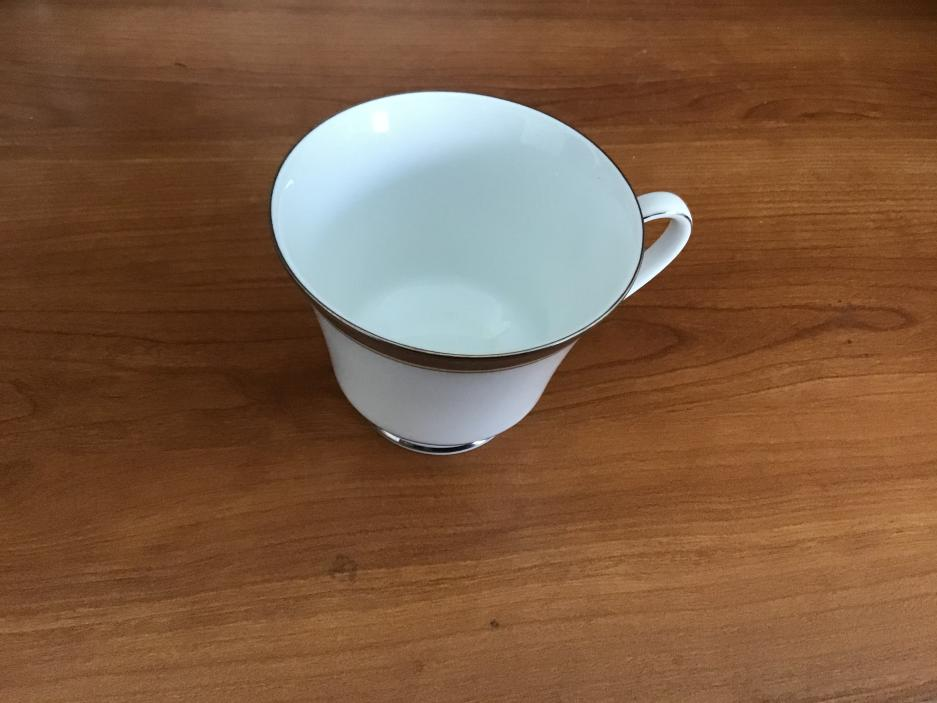
\includegraphics[width=10cm]{teacup.jpg}
\end{center}

The average velocity is given by 
\[\left<v\right> = \int_{0}^{\infty} v f(v)\text{d}v = \sqrt{\frac{8RT}{\pi \mu}}\]
which means that 
\[t = \frac{4m}{\rho \left<v\right> A} = \frac{4m}{\rho_0 A}\sqrt{\frac{\pi \mu}{8R T}} = \frac{m}{\rho_0 A}\sqrt{\frac{2\pi \mu}{RT}}.\]
By the ideal gas law, the vapor pressure can be represented as $\rho_0 = \frac{P\mu}{RT}$ which means that 
\[t = \frac{m}{\rho_0 A}\sqrt{\frac{2\pi \mu}{RT}} = \frac{mRT}{P\mu A}\sqrt{\frac{2\pi \mu}{RT}}= \frac{m}{PA}\sqrt{\frac{2\pi RT}{\mu}}.\]
While the ice is in motion, the astronaut experiences a force given from problem 21 which implies that the astronauts acceleration is (given that the astronauts mass is $M \approx 130\;\mathrm{kg}$):
\[F = \frac{PA}{2}\implies a = \frac{PA}{2M}\]
This means that 
\begin{align*}
L_{\text{acceleration}} = \frac{1}{2}at^2 &= \frac{1}{2}\left(\frac{PA}{2M}\right)\left(\frac{m}{PA}\sqrt{\frac{2\pi RT}{\mu}}\right)^2\\
&= \frac{1}{2}\left(\frac{PA}{2M}\right)\left(\frac{2\pi m^2 RT}{P^2 A^2 \mu}\right) \\
&= \frac{m^2}{2M}\frac{\pi RT}{PA\mu} \\
&= \frac{(0.136\;\mathrm{kg})^2}{2\cdot 130\;\mathrm{kg}}\frac{\pi \cdot 8.3\;\mathrm{J\cdot mol^{-1}\cdot K^{-1}}\cdot 272\;\mathrm{K}}{550\;\mathrm{Pa}\cdot 0.0063\;\mathrm{m^2}\cdot 0.018\;\mathrm{kg/mol}} \approx 88\;\mathrm{m}
\end{align*}
After the astronaut has stopped accelerating, it will be moving at a constant velocity of 
\[v = at = \left(\frac{PA}{2M}\right)\left(\frac{m}{PA}\sqrt{\frac{2\pi RT}{\mu}}\right) = \frac{m}{2M}\sqrt{\frac{2\pi RT}{\mu}} \approx 0.46\;\mathrm{m/s}.\]
The velocity is constant since after sublimation, there are no other external forces acting on the astronaut. Since this is happening in a vacuum, the astronaut could potentially move at a constant velocity until infinity. However, the aim of this problem is to estimate how realistic the method is. This means that we should aim to look at a realistic time that the astronaut travels the extra distance to the space station a distance of $L = 100\;\mathrm{m}$ away. The extra distance travelled will be 
\[L_{\text{velocity}} = v (\tau - t) = \left(\tau - \frac{m}{PA}\sqrt{\frac{2\pi RT}{\mu}}\right)\frac{m}{2M}\sqrt{\frac{2\pi RT}{\mu}}\]
where $\tau$ is the total time of travel. The total length travelled is then 
\[L = L_{\text{acceleration}} + L_{\text{velocity}} = \frac{m^2}{2M}\frac{\pi RT}{PA\mu} + \left(\tau - \frac{m}{PA}\sqrt{\frac{2\pi RT}{\mu}}\right)\frac{m}{2M}\sqrt{\frac{2\pi RT}{\mu}}.\]
We now solve for $\tau$. By substituting values, we yield
\[100 \approx 88 + 0.46(\tau - 35)\implies \tau \approx 252\;\mathrm{s}.\]
This is a realistic amount of time for the total travel, so yes, this method is realistic to use. 


\end{solution}
\begin{solution}{hard}
Consider a control volume that encloses the wave front and moves with it, as shown in figure. To an observer traveling with the wave front, the liquid to the right appears to be moving toward the wave front with speed $u$ and the liquid to the left appears to be moving away from the wave front with speed $u-v$. The observer would think the control volume that encloses the wave front is stationary i.e. a steady flow process.
The continuity relation gives$$uH = (u-v)(H+h)\implies v = u \frac{h}{H+h}$$Also we can say$$ P_{2,avg}A_2-P_{1,avg}A_1 = \dot{m}(-V_2)-\dot{m}(-V_1)$$$$\implies \frac{\rho g(H+h)^2}{2} - \frac{\rho g H^2 }{2} = \rho c_0y(-u + v) - \rho u H(-u)$$$$\implies g \left(1+\frac{h}{2H}\right) h = vu$$Combining the two equations gives
$$u^2 = gH\left(1+\frac{h}{H}\right) \left(1+\frac{h}{2H}\right)$$As $h \ll H$,
$$u= \boxed{\sqrt{gH}}$$
\tcbline
\textbf{A Generalization:} For any given height $h$, the dispersion relationship is:
$$\omega^2 = gk \tanh(kh)$$where $\omega$ is the angular frequency and $k$ is the wavenumber (number of wavelengths per unit distance). For small values, we have $\tanh(kh)=kh$ or:
$$\omega^2 = gk^2h \implies \omega=k\sqrt{gh}$$The speed the waves will be travelling at, or the phase velocity, will be:
$$\boxed{v=\frac{\omega}{k}=\sqrt{gh}}$$For large values of $h$, we have $\tanh(kh)=1$ or:
$$\omega^2=gk \implies v = \sqrt{\frac{g}{k}}$$This tells us that waves with higher wavenumbers (e.g. tsunamis) travel faster than waves with lower wavenumbers.
\end{solution}

\begin{solution}{normal}
Bubble $A$ has a radius $r$ and the pressure difference between the inside and the air is $\Delta p_{A,air}=2\cdot\frac{2\gamma}{r}$. The extra factor of two is because a bubble film essentially has two surfaces. Bubble $B$ has a radius $2r$ and thus the pressure difference between the inside and the air is  $\Delta p_{B,air}=\frac{4\gamma}{2r}$. We now look at the pressure difference between the two bubbles, and we get:
$$\Delta p_{B,A} = 4\gamma\left(\frac{1}{r}-\frac{1}{2r}\right)$$
Therefore, the radius of curvature of the surface in the middle is:
$$\frac{1}{R} = \frac{1}{2r} \implies R = 2r$$
We can assume that the middle surface is in the form of a spherical cap so we can use the formula:
$$A=2\pi R^2(1-\cos\theta)$$
where $\theta$ is the angle that the middle surface subtends. We can determine $\theta$ by drawing a free body diagram. We look at the intersection of the middle film, the film from bubble $A$ and the film from bubble $B$. Since all three films have the same surface tension, the three films must form an angle of $120^\circ$ with each other. With a little bit of geometry, we can show that the angle the middle film subtends is also $\theta=120^\circ$. Therefore, the surface area is:
$$A=2\pi R^2\left(\frac{3}{2}\right) = \boxed{12\pi r^2}$$
\end{solution}

\newpage
\section{Solutions to Revision Problems}
This section will contain problem 55-86 of the handout. Revision problems take concepts and ideas from earlier problems and places them in a new context. As a result, many of the problems in this section will seem familiar. This however, does not mean that all the problems in this section are easy. Some of the hardest problems originate in this section.

\begin{solution}{normal}
\textbf{a)} Let the normal force from the floor on the ladder be $N$. Then, at the cutoff case, the friction force takes on it's maximum, so the friction from the floor is $\mu N$.

\begin{center}
\begin{asy}
size(4cm);
defaultpen(fontsize(10pt));

real wall_th = 0.1, wall_h = 1.1, wall_w = 0.7;
fill((-wall_th, -wall_th)--(-wall_th, wall_h)--(0, wall_h)--(0, 0)--(wall_w, 0)--(wall_w, -wall_th)--cycle, gray(0.8));
draw((0, wall_h)--(0, 0)--(wall_w, 0));

real ladder_w = 0.5, ladder_h = 0.8;
draw((0, ladder_h)--(ladder_w, 0));

draw("$\theta$", arc((ladder_w, 0), 0.08, 180 - aTan(ladder_h/ladder_w), 180));

real N = 1/5, mu = 0.8, eps = 0.02;
draw(Label("$N_2$", Relative(1), dir(0)), shift(ladder_w, 0)*((0, 0)--(0, N)), rgb(0, 0.4, 0), Arrow(TeXHead));
draw(Label("$\mu N$", Relative(1), dir(-90)), shift(ladder_w, -eps)*((0, 0)--(-mu*N, 0)), rgb(0, 0.4, 0), Arrow(TeXHead));
draw(Label("$N_1$", Relative(1), dir(90)), shift(0, ladder_h)*((0, 0)--(mu*N, 0)), rgb(0, 0.4, 0), Arrow(TeXHead));

real mg = N+mu^2*N;
draw(Label("$mg$", Relative(1), dir(190)), shift(ladder_w/2, ladder_h/2)*((0, 0)--(0, -mg)), rgb(0, 0.3, 0.6), Arrow(TeXHead));
\end{asy}
\end{center}

Since the ladder is in equilibrium, we have three equations. These is the equation of equilibrium of force in the horizontal and vertical direction and as well as torques. Looking quickly at the vertical forces, we can see easily that $N_2=mg$. Then by looking at the horizontal forces, we see that $N_1=\mu N$. Therefore, there is only one equation of torque remaining.
\vspace{3mm}

\noindent We first have to find the pivot point of the ladder. Generally, the pivot point of the system is located where there are more forces. Thus, by looking at the ladder, we see that the pivot point of the system is the bottom of the ladder. Balancing the torques due to gravity and $N_1$, we have
$$N_1\ell\sin\theta=mg(\ell/2)\cos\theta\implies N_1=\frac{mg}{2\tan\theta}$$This is also the value of the frictional force $F$ as we have found before. Thus, by using $F\geq\mu{mg}$ we find
$$\frac{mg}{2\tan\theta}\leq\mu{mg}\implies \boxed{\tan\theta\geq\frac{1}{2\mu}}$$

\textbf{b)} Drawing a freebody diagram gives us the following diagram
\begin{center}
\begin{asy}
size(4cm);
defaultpen(fontsize(10pt));

real wall_th = 0.1, wall_h = 1.1, wall_w = 0.7;
fill((-wall_th, -wall_th)--(-wall_th, wall_h)--(0, wall_h)--(0, 0)--(wall_w, 0)--(wall_w, -wall_th)--cycle, gray(0.8));
draw((0, wall_h)--(0, 0)--(wall_w, 0));

real ladder_w = 0.5, ladder_h = 0.8;
draw((0, ladder_h)--(ladder_w, 0));

draw("$\theta$", arc((ladder_w, 0), 0.08, 180 - aTan(ladder_h/ladder_w), 180));

real N = 1/5, mu = 0.8, eps = 0.02;
draw(Label("$N$", Relative(1), dir(0)), shift(ladder_w, 0)*((0, 0)--(0, N)), rgb(0, 0.4, 0), Arrow(TeXHead));
draw(Label("$\mu N$", Relative(1), dir(90)), shift(0, ladder_h)*((0, 0)--(mu*N, 0)), rgb(0, 0.4, 0), Arrow(TeXHead));
draw(Label("$\mu N$", Relative(1), dir(180)), shift(-eps, ladder_h)*((0, 0)--(0, mu^2*N)), rgb(0, 0.4, 0), Arrow(TeXHead));

real mg = N+mu^2*N;
draw(Label("$mg$", Relative(1), dir(190)), shift(ladder_w/2, ladder_h/2)*((0, 0)--(0, -mg)), rgb(0, 0.3, 0.6), Arrow(TeXHead));
\end{asy}
\end{center}
We see that from force balance that there is not an opposite force to oppose the force of $\mu N$ from the wall. This means that it is impossible for the ladder to stay still in this case.
\tcbline
There is an easier way to solve part a. Let us project the gravitational force vector $mg$ and the normal force from the wall $N_1$ such that they meet at a point above the middle of the ladder. At this location, the torque caused by these two forces is zero. In order to be in static equilibrium, the force from the ground must also intersect this point. The slope the force from the ground makes with the horizontal is $2\tan\theta$.

\begin{center}
\begin{asy}
size(4cm);
defaultpen(fontsize(10pt));

real wall_th = 0.1, wall_h = 1.1, wall_w = 0.7;
fill((-wall_th, -wall_th)--(-wall_th, wall_h)--(0, wall_h)--(0, 0)--(wall_w, 0)--(wall_w, -wall_th)--cycle, gray(0.8));
draw((0, wall_h)--(0, 0)--(wall_w, 0));

real ladder_w = 0.5, ladder_h = 0.8;
draw((0, ladder_h)--(ladder_w, 0));

draw("$\theta$", arc((ladder_w, 0), 0.08, 180 - aTan(ladder_h/ladder_w), 180));

real N = 1/5, mu = 0.8, eps = 0.02;
draw(Label("$N_1$", Relative(1), dir(90)), shift(0, ladder_h)*((0, 0)--(mu*N, 0)), rgb(0, 0.4, 0), Arrow(TeXHead));
draw(shift(0, ladder_h)*((mu*N, 0)--(ladder_w/2, 0)), dashed);

draw(Label("$f_\text{ground}$", Relative(1), dir(0)), shift(ladder_w, -eps)*((0, 0)--(-ladder_w/4, ladder_h/2)), rgb(0, 0.4, 0), Arrow(TeXHead));
draw(shift(ladder_w, -eps)*((-ladder_w/4, ladder_h/2)--(-ladder_w/2, ladder_h)), dashed);

real mg = N+mu^2*N;
draw(Label("$mg$", Relative(1), dir(190)), shift(ladder_w/2, ladder_h/2)*((0, 0)--(0, -mg)), rgb(0, 0.3, 0.6), Arrow(TeXHead));
draw(shift(ladder_w/2, ladder_h/2)*((0, ladder_h/2)--(0,0)),dashed);
\end{asy}
\end{center}
Since the force from the ground is consisted of both the normal force $N_2$ and the friction force $f_s$, we have:
$$2\tan\theta=\frac{N_2}{f_s}$$Combining this with $f_s \le \mu N_2$ gives:
$$\boxed{\tan\theta \ge \frac{1}{2\mu}}$$
\end{solution}

\begin{solution}{easy}
Let $d$ denote the common distance of separation between adjacent cars (it's the same for all lanes) \vspace{3mm}

The flow rate (in $\text{cars/s}$) of the cars entering lane $A$ is equal to $\dfrac{v_A}{d}$ \vspace{3mm}

The flow rate (in $\text{cars/s}$) of the cars entering lane $B$ is equal to $\dfrac{v_B}{d}$ \vspace{3mm}

Note that $v_A=3\;\text{km/h}$ and $v_B=5\;\text{km/h}$ \vspace{3mm}

By idea 39, the flow rate (in $\text{cars/s}$) of the cars entering lane $C$ must be $$\dfrac{v_A}{d}+\dfrac{v_B}{d}$$

This means that the velocity of the cars in lane $C$ is simply $$v_A+v_B=8\;\text{km/h}$$

Thus, our final answer is $$\dfrac{1\;\text{km}}{3\;\text{km/h}}+\dfrac{2\;\text{km}}{8\;\text{km/h}}=0.583\;\text{h}=\boxed{35\;\text{min}}$$
\end{solution}
\begin{solution}{normal}
The key insight is noting if the net vertical forces of the normal and friction forces were directed downwards then the stopper would be blocked. Let us then try to calculate the vertical components of forces that are involved. Let the normal force directed on the wedge be $N$. We then know that the vertical component of the normal force is clearly either $N\cos\alpha$ or $N\sin\alpha.$ We can figure the component by chasing angles around, but an easier way is to imagine $\alpha\to 0.$ In this case, the horizontal component of the normal force also goes to zero, which is the behavior of a sine function, so the horizontal component is $N\sin\alpha.$ This in turn means that the vertical component of force involved is $N\cos\alpha$.
\vspace{3mm}

We now try to find the vertical component of friction involved. The friction force directed downwards on the direction of the wedge is $\mu N$ (because $N$ is already perpendicular, you do not have to manipulate it with trigonometric functions). This means that the vertical component of friction is $\mu N\sin\alpha$. 
\vspace{3mm}

We now equate these, with an inequality where the vertical component of the normal force greater than the friction force for the wedge to pass through.
\begin{align*}
N\cos\alpha > \mu N \sin\alpha\\
\boxed{\mu < \cot\alpha}
\end{align*}
\end{solution}

\begin{solution}{normal}
Two forces act on the rod in the vertical direction, it's weight and the force of friction, where at its maximum is $\mu N_1$. As the weight increases, we must have $N_1$ increase as well. Let us look at the limiting case where $W_\text{rod} \to \infty$. The normal and friction forces acting on the cylinder will be so large that the mass of the cylinder will be negligible, thus we can ignore the force $mg$. This allows us to effectively turn gravity off.
\vspace{2mm}

Let us now rotate the setup by an angle $\alpha/2$ such that it is completely symmetrical  along its vertical axis. It is clear that the horizontal forces will cancel each other out.
\begin{center}
    \begin{asy}
    size(5cm);
draw(circle((0,0),3));
draw((-2.62,-1.47)--(-0.59,-0.33),EndArrow);
draw((-2.62,-1.47)--(-0.59,-5.07),EndArrow);

draw((2.62,-1.47)--(0.59,-0.33),EndArrow);
draw((2.62,-1.47)--(0.59,-5.07),EndArrow);
    \end{asy}
\end{center}

Now we just have to balance out vertical forces. Due to symmetry, the y-component of each friction force cancels out with the y-component of each normal force. For the left side, we have:
$$N_1\sin(\alpha/2)=\mu_1 N_1\cos(\alpha/2) \implies \boxed{\mu_1 > \tan(\alpha/2)}$$
We have the inequality since the force balance equation gives the maximum friction. Similarly for the other side:
$$\boxed{\mu_1 > \tan(\alpha/2)}$$
\end{solution}

\begin{solution}{normal}\textbf{(a)} In analogy to electrical circuits, the resistance of a single wire is given by:
$$R = \frac{L}{\kappa S}$$
Since we have four wires in parallel, the effective resistance is:
$$R = \frac{L}{4\kappa S}$$
\vspace{3mm}

\noindent \textbf{(b)} For a small period of time $\text{d}t$, the temperature is changed by $\Delta T$ degrees. This means that 
\[P \equiv \frac{\text{d}Q}{\text{d}t} = C\Delta\dot{T}.\]
Let us look at the electrical analogy between heat conduction and electric circuits. In this case, $\dot{Q}$ acts as the current while the temperature difference $\Delta T \equiv T - T_0$ acts as the voltage difference. From this perspective, we can also define 
\[\dot{Q} = \frac{\Delta T}{R}.\]
This means that from adding these two individual expressions (as there is an extra $\dot{Q}$ due to our "voltage difference") we have that 
\[P\cos \omega t = C\Delta\dot{T} + \frac{\Delta T}{R}.\]
As power varies with time, we attempt to seek the solution in the form of 
\[T = T_0 + \Delta T \sin (\omega t + \phi).\]
Taking the derivative of our sought solution and substituting into our differential equation gives us 
\[P\cos\omega t = C\Delta T\omega \cos (\omega t + \phi) + \frac{\Delta T}{R}\cos \left(\omega t + \phi - \frac{\pi}{2}\right)\]
which can be seen as the sum of multiple rotating vectors or:
\[\vec{P} = \vec{P}_C + \vec{P}_R.\]
Each of these vectors have an individual magnitude of 
\[P_C = C\Delta T \omega, \quad P_R = \frac{\Delta T}{R}\]
\begin{center}
    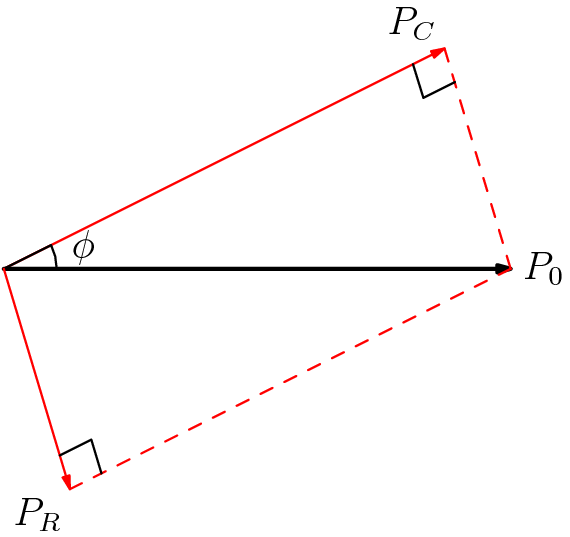
\includegraphics[width=6cm]{phasor.png}
\end{center}
Therefore, from pythagorean theorem, the amplitude of oscillations is 
\[P_0^2 = (C\omega\Delta T)^2 + \left(\frac{\Delta T}{R}\right)^2\implies \Delta T = \frac{P_0}{\sqrt{C^2\omega^2 + R^{-2}}}.\]
Our solution is in the form of 
\[T = T_0 + \Delta T \sin (\omega t + \phi) = T_0 +  \frac{P_0\cos (\omega t + \phi)}{\sqrt{C^2\omega^2 + R^{-2}}}.\]
Let us estimate the phase difference. We can go back to our phase diagram and see that 
\[\phi = \arcsin\left(\frac{P_C}{P_0}\right) = \arcsin\left(\frac{C\omega}{\sqrt{C^2 \omega^2 + R^{-2}}}\right).\]
This means that our final solution is 
\[T = T_0 +  \frac{P_0\cos \left(\omega t + \arcsin\left(C\omega/\sqrt{C^2 \omega^2 + R^{-2}}\right)\right)}{\sqrt{C^2\omega^2 + R^{-2}}} .\]
\vspace{3mm}

\noindent \textbf{(c)} Remember from part b that our amplitude of oscillations of $\Delta T$ is given by $\Delta T = \frac{P_0}{\sqrt{C^2\omega^2 + R^{-2}}}$. We want there to be as large a change as possible with a small change in $C$. This is equivalent to maximizing the derivative ie setting the double derivative to $0$. Upon taking two derivatives, we get the function
\[\frac{3P_0 C^2 \omega^4}{(C^2 \omega^2 + R^{-2})^{5/2}} - \frac{P_0 \omega^2}{(C^2 \omega^2 + R^{-2})^{3/2}} = 0.\]
Seperating and solving for $\omega$ yields $\omega = 1/\sqrt{2}CR$.
\vspace{3mm}

\noindent \textbf{(d)} As the questions asks to estimate, we ignore all numerical prefactors. From part c), we know that $C \approx 1/\omega R$. This should be of the same order as the heat capacity of the bridges. Therefore, we have 
\[\frac{1}{l/\kappa S\cdot \omega} = \rho lSc\implies \omega_c \approx \frac{\kappa}{c\rho L^2}.\]
\end{solution}
\begin{solution}{normal}
Similar to problem 16, we want:
$$\rho gh(\pi R^2) = mg + V\rho g$$
except this time:
\begin{align*}
V &= \frac{2}{3}\pi R^3 - \pi H^2\left(R-\frac{H}{3}\right) \\
&= \frac{2}{3}\pi R^3 - \pi (R-h)^2\left(\frac{2R+h}{3}\right) \\
&= \frac{2}{3}\pi R^3 - \frac{\pi}{3} (2R^3+R^2h-4R^2h-\cancel{2Rh^2}+\cancel{2Rh^2}+h^3) \\
&= \pi R^2h - \frac{\pi}{3}h^3
\end{align*}
Plugging this in gives:
$$\cancel{\rho gh(\pi R^2)} = mg +  \cancel{\pi R^2h\rho g} - \frac{\pi}{3}h^3\rho g$$
or:
$$mg = \frac{\pi}{3}h^3\rho g \implies \boxed{h = \sqrt[3]{\frac{3m}{\pi \rho}}}$$
Verifying, if we plug $m=\frac{\pi}{3}\rho R^3$, we do indeed get $h=R$.
\end{solution}

\begin{solution}{normal}
Assume the water surface pressure uniform. In the rotating frame of the water, every water element is at rest. So in this rotating frame, the hydrostatics equation is$$\vec{F} + \vec{F}_{\text{centrifugal}} - \vec{\nabla} P = 0$$where $\vec{F} = -\rho g \hat{j}$ is the force on the body per unit volume, $\vec{F}_{\text{centrifugal}}$ the centrifugal force, and $- \vec{\nabla} P$ is the force due to the pressure gradient.
\begin{center}
\hspace{4em}
\begin{asy}
import graph;
size(10cm); 
real labelscalefactor = 0.5; /* changes label-to-point distance */
pen dps = linewidth(0.7) + fontsize(10); defaultpen(dps); /* default pen style */ 
pen dotstyle = black; /* point style */ 
real xmin = -1.0677692311141869, xmax = 4, ymin = -1.2587115300623306, ymax = 0.9619427617015781;  /* image dimensions */

 /* draw figures */
real parabola1 (real x) {return x^2/2/0.5;} 
draw(shift((0,0.25))*rotate(0)*graph(parabola1,-3,3)); /* parabola construction */
draw((0,1)--(0,-1), linetype("2 2")); 
draw((1.2,-0.4)--(0.8,0.4),EndArrow(6)); 
draw((1.2,-0.4)--(1.2,-1.2), EndArrow(6)); 
draw((1.2,-0.4)--(1.8,-0.4), EndArrow(6)); 
label("$-\vec{\nabla}P$",(1.0104163055295856,0.1659760211390613),SE*labelscalefactor); 
label("$\vec{F}_c$",(1.4,-0.2),SE*labelscalefactor); 
label("$\vec{F}=-\rho g \hat{j}$",(1.2303137319106705,-0.7569737402914056),SE*labelscalefactor); 
label("$\vec{R}$",(0.5799128933187296,-0.7),SE*labelscalefactor); 
draw((0,-0.4)--(1.2,-0.4),  linetype("2 2"),EndArrow(6)); 
draw((0,-1)--(1.2,-0.4), linetype("2 2"),EndArrow(6)); 
label("$\vec{x}$",(0.47460990040384404,-0.2304587757169782),SE*labelscalefactor); draw(shift((0,0.9))*rotate(0)*xscale(0.10437759946869621)*yscale(0.029911256590888294)*unitcircle,linetype("2 2")); 
draw((0.035919890681460606,0.8372879118687089)--(0.09913820101098883,0.8516557096708743),EndArrow(6)); 
label("$\omega$",(0.05,0.80),SE*labelscalefactor); 
 /* dots and labels */
clip((xmin,ymin)--(xmin,ymax)--(xmax,ymax)--(xmax,ymin)--cycle); 
\end{asy}
\end{center}
Clearly, by definition we have $\vec{F}_{\text{centrifugal}} = -\rho\vec{\omega} \times (\vec{\omega} \times \vec{R})$, hence the hydrostatic equation becomes$$\vec{\nabla} P = - \rho g \hat{j} + \rho \omega^2 x \hat{i}$$$$\Rightarrow \frac{\partial{P}}{\partial{x}} = \rho \omega^2 x  \ \ \ ; \ \ \frac{\partial{P}}{\partial{y}} = -\rho g$$Integrating, we have$$P = \frac{\rho \omega^2 x^2}{2} - \rho g y$$And assuming the surface pressure constant, this yields$$\frac{\rho \omega^2 x^2}{2} = \rho g y \Rightarrow y = \frac{{\omega}^2}{2g} x^2$$Thus the cross sectional surface of the rotating water is a parabola with this equation
Hence substituting $x=R$ gives the relative height near the edges of the vessel, which is just$$\Delta{h} = \boxed{\frac{{\omega}^2}{2g} R^2}$$
\tcbline
\textbf{Solution 2:} Consider a water particle on the surface. In the rotating frame, it experiences three forces, a gravitational force downwards, a centrifugal force outwards, and a normal force perpendicular to the surface.
\begin{center}
\begin{asy}
import graph; usepackage("amsmath"); size(8cm); 
real labelscalefactor = 0.5; /* changes label-to-point distance */
pen dps = linewidth(0.7) + fontsize(10); defaultpen(dps); /* default pen style */ 
pen dotstyle = black; /* point style */ 
real xmin = -2.3, xmax = 2.3, ymin = -0.6303276899786796, ymax = 1.8007701906158518;  /* image dimensions */

 /* draw figures */
draw((-0.004788462906506731,1.5657454104578188)--(-0.004788462906506731,-0.4342545895421811),  linetype("2 2")); draw(shift((-0.010691339830682305,1.477332350856711))*rotate(0)*xscale(0.10437759946867764)*yscale(0.02991125659088297)*unitcircle,  linetype("2 2")); 
draw((0.04126556059680052,1.4520399521327993)--(0.10448387092632873,1.4664077499349646), EndArrow(6)); 
label("$\omega$",(0.030417105307975936,1.45),SE*labelscalefactor); 
real f1 (real x) {return 0.3*x^(2);} 
draw(graph(f1,-2.1804603169924706,2.4108271552649447)); 
draw((1.40372705181681,0.5911348908006938)--(0.8069949759983192,1.2137966803862708),EndArrow(6)); 
draw((1.40372705181681,0.5911348908006938)--(1.3998783666087462,-0.005988000295837015),EndArrow(6)); 
draw((1.40372705181681,0.5911348908006938)--(2.070516955987754,0.6014744900836987),EndArrow(6)); 
label("$m\omega^2r$",(1.6714929410231147,0.85),SE*labelscalefactor); 
label("$mg$",(1.4273659571977222,0.32922698255723726),SE*labelscalefactor); 
label("$N$",(1.1,1.1),SE*labelscalefactor); 
 /* dots and labels */
dot((1.40372705181681,0.5911348908006938),dotstyle); 
clip((xmin,ymin)--(xmin,ymax)--(xmax,ymax)--(xmax,ymin)--cycle); 
 /* end of picture */
\end{asy}
\end{center}

The three forces must sum up to zero. If we add them geometrically, they form a closed right angle triangle
\begin{center}
\begin{asy}
import graph; usepackage("amsmath"); size(5cm); 
real labelscalefactor = 0.5; /* changes label-to-point distance */
pen dps = linewidth(0.7) + fontsize(10); defaultpen(dps); /* default pen style */ 
pen dotstyle = black; /* point style */ 
real xmin = -9.090168863933378, xmax = 6.292596815605005, ymin = -3.029927271486699, ymax = 5.03253105616609;  /* image dimensions */

 /* draw figures */
draw((-5,3)--(0,3), EndArrow(6)); 
draw((0,3)--(0,0), EndArrow(6)); 
draw((0,0)--(-5,3),EndArrow(6)); 
draw(shift((-5,3))*xscale(1.2159249686603875)*yscale(1.2159249686603875)*arc((0,0),1,-30.963756532073518,0)); 
label("$m\omega^2r$",(-2.5,3.5),SE*labelscalefactor); 
label("$mg$",(0.08551592737021871,1.9739694590648924),SE*labelscalefactor); 
label("$N$",(-2.6806831641257185,1.4),SE*labelscalefactor); 
label("$\theta$",(-3.760175492514377,2.8),SE*labelscalefactor); 
 /* dots and labels */
clip((xmin,ymin)--(xmin,ymax)--(xmax,ymax)--(xmax,ymin)--cycle); 
 /* end of picture */
\end{asy}
\end{center}
where $\tan\theta=\frac{g}{\omega^2 r}$
Since the normal force is perpendicular to the surface, the slope of the surface at this point is:
$$\frac{dh}{dr}=\cot\theta = \frac{\omega^2r}{g}$$Integrating, from $0$ to $R$, we get:
$$\boxed{\Delta h = \frac{\omega^2R^2}{2g}}$$
\end{solution}

\begin{solution}{hard}\textbf{(a)} By idea 1, note that 
\[P \equiv \frac{\text{d}Q}{\text{d}t} = C\frac{\text{d}T}{\text{d}t}.\]
Therefore, by rearranging, we have that 
\[T = \int_{T_0}^{T_1} \text{d}T = \int_{0}^{\tau} \frac{P}{C} \text{d}t\implies C = \frac{P\tau}{T_0 - T_1} = 360\;\mathrm{J/^{\circ}C}.\]
\vspace{3mm}

\noindent \textbf{(b)} The delay in the change of temperature reading and the inital rise in temperature is due to the sensor's surroundings not initially heating up. By the definition of heat capacity, an infintesimal amount of heat that is transfered to the system is 
\[\text{d}Q = -C\text{d}\bar{T}.\]
After the temperature of the sensor's surroundings and the plate become equal, the heat dissipated by the plate is given by 
\[\kappa (T - T_{\text{amb}}) = -C \frac{\text{d}T}{\text{d}t}\implies \ln (T - T_{\text{amb}}) = -\frac{\kappa t}{C} + m\]
where $m$ is an arbritary constant. Before the sink recieves heat $Q$, it's temperature must be be the ambient temperature as the electrical component has been switched off for a long time. Theoretically, we assume that the temperature of the whole plate and sensor is the same right after $t = 0$ for our equation to be valid for the entire duration (although realistically it is valid only after some time). Let this temperature be $T_2$.  Then we have that 
\[Q = C (T_2 - T_{\text{amb}})\]
and therefore our goal is to determine the value of $m$ from the graph given. Our solution of $\Delta T \equiv T_2 - T_{\text{amb}}$ will be exponential or $e^m$. From the table, it is clear that $T_{\text{amb}} = 20^{\circ}\;\mathrm{C}$. Therefore, we plot our graph with $y \equiv \ln (T - T_{\text{amb}})$ and $x \equiv t$. From the graph drawn, we find $m = 4.73$ and therefore, $Q = 41\;\mathrm{kJ}$.
\end{solution}
\begin{solution}{normal}
In the freefalling frame, both balls move with a constant velocity. Let us define point $Q$ as where both $A$ and $B$ are an equal distance from each other. 
\vspace{3mm}

To find where $Q$ is, we can connect line $|AB|$ and find the perpendicular bisector (which can be done using a compass and a straight-edge). We also draw a vertical line down $P$. $Q$ is found where this line and $|AB|_{\perp}$ connects. 
\vspace{3mm}

In the lab frame, $Q$ is freefalling and thus after a time $t$ it has fallen a distance $|PQ| = gt^2/2$. We know measure and see that 
\[|PQ| = 8.6\;\mathrm{cm},\hspace{10pt} |AQ| = 26\;\mathrm{cm}\]
we now find that 
\[|PQ| = \frac{1}{2}gt^2\implies t=1.3\;\mathrm{s}\]
and using $d = vt$ (because of a constant acceleration), we find that 
\[|AQ| = 1.3v\implies v \approx \boxed{20\;\mathrm{m/s}}\]
\end{solution}
\begin{solution}{normal}
An ideal-gas cycle consisting of two isotherms at temperatures $T_1$ and $T_2$, and two isochores joining them will look like:
\begin{center}
\begin{asy}
unitsize(2cm);
import graph;
draw((0, 0)--(0, 4), arrow=Arrow(TeXHead), linewidth(1));
draw((0, 0)--(4,0), arrow=Arrow(TeXHead), linewidth(1));

label("$P$", (0, 4), NW);
label("$V$", (4, 0), SE);

draw((0.5, 3.5).. (2, 2.5).. (3.5, 2));
label("$T_2$", (3.5, 2), E);
draw((0.5, 2.1).. (2, 1.1).. (3.5, 0.6));
label("$T_1$", (3.5, 0.6), E);
draw((1, 1.71) -- (1, 3.1), linewidth(1));
draw((1, 1.71)..(2, 1.1)..(3, 0.72), linewidth(1));
draw((1, 3.1)..(2, 2.5)..(3, 2.13), linewidth(1));
draw((3, 0.72) -- (3, 2.13), linewidth(1));

label("2", (1, 1.71), SW);
label("1", (3, 0.72), S);
label("3", (1, 3.1), NE);
label("4", (3, 2.13), N);

draw((0.2, (1.71 + 3.1)/1.9) -- (0.7, (1.71 + 3.1)/1.9), arrow=Arrow(8));
label("$Q_1$", (0.7, (1.71 + 3.1)/1.9), N);
draw((3.2, 1.2) -- (3.7, 1.2), arrow=Arrow(8));
label("$Q_3$", (3.7, 1.2), N);
draw((2, 3.3) -- (2, 2.7), arrow=Arrow(8));
label("$Q_2$", (2, 2.7), E);
draw((2, 1.3) -- (2, 0.8), arrow=Arrow(8));
label("$Q_4$", (2, 0.8), W);

draw((1, 0) -- (1, 0.1));
draw((3, 0) -- (3, 0.1));

label("$V_1$", (1, 0), S);
label("$V_2$", (3, 0), S);
\end{asy}
\end{center}
Since there are no adiabatic processes, heat will be lost on every step. For isochoric processes on $2\to 3$ and $1\to 4$, the heat released will be 
\begin{align*}
Q_1 &= C_V R (T_2 - T_1) \\
Q_3 &= C_V R (T_1 - T_2)
\end{align*}
For isothermal processes on $1 \to 2$ and $3 \to 4$, the heat released will be 
\begin{align*}
Q_2 &= RT_2 \ln \frac{V_2}{V_1} \\
Q_4 &= -RT_1 \ln \frac{V_1}{V_2}
\end{align*}
The heat released during cooling feeds the heating isochore. Therefore, the work done is the change in heat along both isotherms or:
\[W = Q_2 - Q_4.\]
The efficiency of the cycle will be given by 
\[\eta = \frac{W}{Q_2} = \frac{Q_2 - Q_4}{Q_2} = 1 + \frac{T_1 \ln \frac{V_1}{V_2}}{T_2 \ln \frac{V_2}{V_1}} = \boxed{1 - \frac{T_1}{T_2}}.\]
\end{solution}
\begin{solution}{normal}
\textbf{(a)} The total heat energy will be given by $Q = nq$ where $n$ is the number of moles and $q$ is the heat. Note that for a heat differential, $\text{d}q = C_v \text{d}T$ holds true. By integrating over we find that 
\[q = \int C_v \text{d}T \approx 550R.\]
The number of moles will be given by the mass over the molar mass or 
\[n = \frac{a^3 \rho}{M} \approx 0.1 \;\mathrm{mol}.\]
Multiplying these two values together gives us approximately $520\;\mathrm{J}$.
\vspace{3mm}

\noindent \textbf{(b)} Consider a photon radiated from the cube. It caries a momentum $p = E_{\perp}/c$ where $E = hf$. Let us assume that the photon initially imparts at an angle $\theta$. The parallel momentum is given by 
\[p_{\parallel} = \frac{E_{\perp}}{c}\cos\theta.\]
Note that the intensity of light is proportional to $\cos \theta$ by Lambert's law. Since intensity is proportional to frequency, the momentum averaged over all directions is 
\[\left<p_{\parallel}\right> = \int_{0}^{\pi} \frac{E_{\perp}}{c}\cos^2\theta \text{d}\Omega\]
where $\text{d}\Omega = 2\pi \sin \theta \text{d}\theta$ is the solid angle. Integrating this tells us that 
\[\left<p_{\parallel}\right> = \frac{E_{\perp}}{3c} = \frac{Q}{3c}.\]
The mass of the cube is $a^3 \rho$ so, the velocity is given by 
\[v = \frac{Q}{3a^3 \rho c}.\]
\vspace{3mm}

\noindent \textbf{(c)} By Stefan-Boltzmann Law, we have that 
\[\frac{P}{A} = \sigma T^4\]
and by idea 1:  
\[P \equiv \frac{\text{d} Q}{\text{d} T} = C\frac{\text{d} T}{\text{d} t}.\]
This means that 
\[ C \text{d} T = \sigma T^4 \text{d} t\implies T^3 \text{d} T = \sigma T^4 \text{d} t.\]
Separating the differential equation tells us 
\[\frac{\text{d} T}{T} = -Bt \implies T = A\cdot e^{-B t}.\]
\vspace{3mm}

\noindent \textbf{(d)} We can estimate the momentum imparted upon the cube will be equal to the heat energy over the average velocity of the hydrogen molecules. In other words, 
\[a^3 \rho v = \frac{Q}{v_H} = Q\sqrt{\frac{M_H}{RT}}\implies v = \frac{Q}{a^3 \rho}\sqrt{\frac{M_H}{RT}}.\]

\end{solution}
\begin{solution}{hard}
The total light emission power of the LED is $P_0 = 1 \mu W$. 
\begin{center}
    \begin{asy}
    unitsize(2cm);
    draw(circle((0,0), 0.75));
label("LED", (0,0));
draw((-2, 0) -- (-0.75, 0), arrow=Arrow(4));
label("$W$", (-1.2, 0), N);
draw((0, -2) -- (0, -0.75), arrow=Arrow(4));
label("$Q$", (0, -1.35), E);
draw((0, 0.75) -- (0, 2), arrow=Arrow(4));
label("$Q'$", (0, 1.75), E);
    \end{asy}
\end{center}
Since we have $$\frac{P_0}{A} = \int_{\nu_1}^{\nu_2}{I(\nu, T)} \mathrm{d}\nu$$ We substitute the well known expression for $I(\nu, T)$ from Planck's radiation law: 
$$ \frac{P_0}{A} = \int_{\lambda_1}^{\lambda_2}{\frac{2\pi h c^2 \mathrm{d}\lambda}{\lambda^5(e^{\frac{hc}{\lambda k T}} - 1)}} = \frac{2\pi h}{c^2} \int_{\nu_1}^{\nu_2}{\frac{\nu^3}{e^{\frac{h\nu}{kT_0}}-1} \mathrm{d}\nu}$$ We can use the well known integral $$\int_{0}^{\infty}{\frac{\eta^3\text{d}\eta}{e^\eta - 1}} = 6\xi(4) = \frac{\pi^4}{15}$$ and substitute the known values and using the problem condition. We find from evaluating the integral that $T_1 \geq 1116 K$. Now, the maximum possible efficiency of the LED is just $$\eta_{\text{max}} = \frac{T_1}{T_1 - T_0} -1 = 1+ 0.354 = \boxed{1.354}$$

\end{solution}
\begin{solution}{normal}
Consider the reference frame moving with velocity $v$ to the right. This frame is easier to work with because here the end of the rod on the ground is at rest. Let's call this end $A$. Let $t=0$ correspond to the time when the rod is vertical. At time $t$, the distance between $A$ and the vertical wall is $d=vt$. Let the angle between the rod and horizontal wall be
$$\theta = \frac{\pi}{2}-\alpha$$
such that
$$\cos \theta = \frac{vt}{2l}$$
Differentiating with respect to time gives
$$\dot \theta \sin \theta= \frac{v}{2l} \implies \dot \theta = \frac{v}{2l \sin \theta}$$

The velocity of the sphere is
$$\dot \theta (2l-x) = \frac{v(2l-x)}{2l \sin \theta}$$
perpendicular to the rod. Therefore, the $x-$ component of the velocity
$$v_x = \frac{v(2l-x)\sin \theta}{2l \sin \theta} = \frac{v(2l-x)}{2l }$$
is constant, implying that $a_x = 0$. Now the centripetal acceleration of the sphere
$$a_c= \dot \theta^2 (2l-x) = \frac{v^2(2l-x)}{4l^2 \sin^2 \theta}$$
which is pointed towards $A$. We know that the acceleration is entirely in $y$, as $a_x = 0$. As a result:
\begin{align*}
a \sin \theta &= \frac{v^2(2l-x)}{4l^2 \sin^2 \theta} \\
a &= \frac{v^2(2l-x)}{4l^2 \sin^3 \theta} \\
  &=\frac{v^2(2l-x)}{4l^2 \cos^3 \alpha}  \\
 &= \frac{v^2}{2l \cos^3 \alpha}(\frac{x}{2l}-1)
\end{align*}
which is pointed in negative $y$ direction. By Newton's second law, we have:
$$N = mg - ma \implies \boxed{N=m(g-\frac{v^2(2l-x)}{\sqrt2 l^2})}$$
\tcbline
\textbf{Solution 2:} We solve it for the general case. Let the place where both walls meet be the origin then we can write the coordinates of sphere as
$$X= x_1-x\sin\alpha$$
$$Y= y_1-x\cos\alpha$$
Now differentiating $Y$ with respect to time we get
$$ v_y=v\tan\alpha-v\tan\alpha\left(\frac{x}{2\ell}\right)$$
Now again differentiating it with respect to time we get
$$a_y=\omega v\sec^2\alpha\left(\frac{x}{2\ell}-1\right)$$
Also we have
$$\omega=\frac{v}{2\ell\cos\alpha}$$
Substituting it we get $$a_y=\frac{v^2}{2\ell}{\sec^3\alpha}\left(\frac{x}{2\ell}-1\right)$$
Now using Newton’s law in $y$ direction we get
$$4mg-N=ma_y$$
Solving we get
$$N=m\left(g-v^2\frac{(2\ell-x)}{l^2\sqrt2}\right)$$
Note that $a_x=0$. Since $\displaystyle v_x=v\left(1-\frac{x}{2l}\right)$ is constant, therefore the rod/sphere will apply no force on each other in the horizontal direction.
\end{solution}

\begin{solution}{hard}
Let us analyze a small section $dz$ in the atmosphere with density $\rho$. The relation between pressure and density is then given by 
\[\dd p = - \rho g \dd z.\]
We know that $p = n k_B T$ and $\rho = nm$ where $m$ is the mass of a single molecule and therefore, 
\[\dv{p}{z} = - \frac{mg p}{k_B T}\implies T \frac{\dd p}{p} = - \frac{mg}{k_B}dz.\]
Note that 
\[p^{1 - \gamma} T^{\gamma} = \text{const.}\]
and therefore, 
\[(1 - \gamma) \frac{\dd p}{p} + \gamma \frac{\dd T}{T} = 0.\]
Now substituting gives us 
\[\frac{\dd T}{\dd z} = -\left(\frac{\gamma - 1}{\gamma}\right) \frac{mg}{k_B} \implies \dd T =  -(1 - \gamma^{-1}) \frac{\mu g}{R}\dd z.\]
Integrating from $T_0$ to $T$ gives us 
\[\int_{T_0}^{T} \dd T = \int_{0}^{z} -(1 - \gamma^{-1}) \frac{\mu g}{R}\dd z \implies \boxed{T = T_0 - (1 - \gamma^{-1}) \frac{\mu g z}{R}}.\]

\end{solution}
\begin{solution}{normal}
The centre of mass of the system is initially on the pulley. In the horizontal direction, the net external force is provided by the tension forces (pulley), and it is always rightwards. (For the block to have covered an angle $\alpha$, the net horizontal force is $\vec{F_{\text{ext}}} = T(1- \cos{\alpha}) \hat{i}$ which is always in positive $\hat{i}$ direction. Hence the centre of mass moves right to the pulley throughout the motion. At the time of collision, it is thus right of the pulley, which is only possible if the \textbf{left block} reaches the pulley first.\footnote{This problem came in the Moscow physics olympics in the 1970s, and is also in the book 'Aptitude Test Problems in Physics by S.S. Krotov. It is quite a famous problem.}
\end{solution}

\begin{solution}{normal}
\textbf{(a)} The internal energy will be given by 
\[U=\mu C V \Delta T=\mu C\left(\frac{4}{3} \pi R^{3}\right)\left(T_{c}-T_{0}\right) \approx 16768\;\mathrm{J}.\]
\vspace{3mm}

\noindent \textbf{(b)} By Fourier's Law,
$$J=\dot{Q}=\kappa\frac{\Delta T}{R}=\frac{\kappa \left(T_{1}-T_{0}\right)}{R} \approx 2458 \;\mathrm{W/m^2}
$$
\vspace{3mm}

\noindent \textbf{(c)} Heat is transferred to the egg via its surface
$$
P=J \times 4 \pi R^{2}=\left[4 \pi K R\left(T_{1}-T_{0}\right)\right] \approx 19.3 \;\mathrm{W}
$$
\vspace{3mm}

\noindent \textbf{(d)} Power is equal to the change in internal energy over time or:
\[P=\frac{d U}{d t} \approx \frac{\Delta U}{\Delta t} \Rightarrow \Delta t=\frac{\Delta U}{P}=\frac{\mu c\left(\frac{4}{3} \pi R^{3}\right)\left(T_{c}-T_{0}\right)}{4 \pi \kappa R\left(T_{1}-T_{0}\right)}.\]
This means that 
\[\tau=\frac{\mu C R^{2}}{3 K}\left(\frac{T_{c}-T_{0}}{T_{1}-T_{0}}\right) \approx 869\;\mathrm{s}.\]
\end{solution}
\begin{solution}{normal}
Note that due to the fact that the thread is extremely long,  there are no horizontal forces exerted by the string and as a result, the horizontal momentum is conserved. We have:
$$mv=(M+m)u$$
Conservation of energy then gives:
$$\frac{1}{2}mv^2 = \frac{1}{2}(M+m)u^2 = mg\ell \implies \frac{1}{2}mv^2 = \frac{1}{2}\frac{m^2v^2}{M+m}+mg\ell$$
Solving for $v$, we get:\footnote{It is good to check for limiting cases. If $m/M \to 0$, we can ignore the horizontal components of velocity and just conserve energy. We get the standard result $v=\sqrt{2g\ell}$. If $M \to \infty$, then we need to provide an infinite speed to raise the height as we stated the string is extremely long.}
$$v=\sqrt{2g\ell\left(1+m/M\right)}$$
\end{solution}

\begin{solution}{normal}
We use idea 51 and list out all the possible combinations of objects moving together. Let us label the surface between the top two masses as $S_1$ and the surface between the bottom two as $S_2$. We have a few options:
\begin{itemize}
    \item $S_1$ static, $S_2$ static
    \item $S_1$ kinetic, $S_2$ static
    \item $S_1$ static, $S_2$ kinetic
    \item $S_1$ kinetic, $S_2$ kinetic 
\end{itemize}
(1) Let us look at the first case. If this is the case, then we have:
$$F=3ma \implies a=\frac{F}{3m}$$
To analyze the conditions for this to occur, we must look at the friction forces. The second block experiences two friction forces from two surfaces. Both forces $f_1$ and $f_2$ have to satisfy $f_1 < mg\mu$ and $f_2 < 2mg\mu$. Since the first condition is harder to meet (and if met, the second one is also met), we will look at the first surface. The top-most block experiences two forces, a force of tension with magnitude $F/2$ and a friction force $-f_1$. Combined together, these forces give the bottom block the acceleration calculated above. We have:
$$m\left(\frac{F}{3m}\right)=\frac{F}{2}-f_1 \implies f_1 = \frac{F}{6}$$
Using the inequality $f_1 < mg\mu$ we get the condition:
$$\frac{F}{6} < mg\mu \implies \frac{F}{mg\mu} < 6$$
\vspace{3mm}

(2) Now let's look at the second case where the bottom two blocks stay together but the top two blocks slide against each other. We wish to balance forces on the bottom two blocks together, but we need to be careful of which direction the friction force points. The top block and the bottom two blocks are both being pulled by a string but since the top block is lighter, it will be pulled faster. As a result, the kinetic friction the top two blocks experiences points directly to the right. Balancing forces, we have:
$$(2m)a=\frac{F}{2}+mg\mu \implies a = \frac{F}{4m}+\frac{1}{2}g\mu$$
\vspace{3mm}

The conditions that has to be met in order for this to take place is: $f_1 = mg\mu$ and $f_2<2mg\mu$. For the second to be satisfied, we can balance forces for the bottommost block. Balancing forces, we have:
$$m\left(\frac{F}{4m}+\frac{1}{2}g\mu\right)=\frac{F}{2}-f_2 \implies f_2 =\frac{F}{4}-\frac{1}{2}mg\mu$$
Using the condition $f_2 < mg\mu$, we get:
$$\frac{F}{mg\mu} < 10$$
For the first condition to be met, we must have $\frac{F}{mg\mu}>6$, if this was not the case, then all three blocks would start sliding together. We can prove this by balancing forces on the middle block. We have:
$$m\left(\frac{F}{4}+\frac{mg\mu}{2}\right)=f_1+f_2 \implies \frac{F}{4}-f_1+\frac{mg\mu}{2} < mg\mu$$
Setting $f_1=mg\mu$ and isolating for $F$ does indeed give us:
$$\frac{F}{mg\mu}>6$$
\vspace{3mm}

(3) This is impossible. If the friction is strong enough such that the top two blocks can move together, then it must be so that the friction is strong enough the bottom two blocks can move together. This is because the normal force between the bottom two blocks will always be stronger than the normal force between the upper two blocks.
\vspace{3mm}

(4) This is an easy case. Balancing forces directly on the second block, we get:
$$ma=f_1+f_2=mg\mu+2mg\mu \implies a=3g\mu$$
This is the case when the applied force crosses the upper boundary set above, which was $\frac{F}{mg\mu}<10$. Therefore, complete slipping occurs when $$\frac{F}{mg\mu} > 10$$
\vspace{3mm}

Finally, we can summarize our results:
$$
\boxed{
a=
\begin{cases}
\frac{F}{3m} & \frac{F}{mg\mu} < 6 \\
\frac{F}{4m}+\frac{g\mu}{2} & 6<\frac{F}{mg\mu}<10 \\
3g\mu & \frac{F}{mg\mu} > 10
\end{cases}
}
$$
\end{solution}

\begin{solution}{normal}
\textbf{A-i)} The buoyant force is going to be: $$F=\rho_\text{air}V_\text{balloon}g$$
where $\rho_\text{air}=\frac{PM_A}{RT}$ from the ideal gas law. Applying the ideal gas law to inside the balloon gives:
$$RT = \frac{(P+\Delta P)V}{n}$$
Therefore, the buoyant force is:
$$\frac{P}{P+\Delta P}nM_Ag$$
\vspace{3mm}

\noindent \textbf{A-ii)} We know that $\rho = \frac{PM_{A}}{RT} \implies \rho = \frac{PM_Az_0}{RT_0(z_0-z)}$. The differential change in pressure for a differential change in height $\mathrm{d}z$ is $$\mathrm{d}P = -\rho g\mathrm{d}z \implies \mathrm{d}P = -\frac {PM_Az_0g}{RT_0(z_0-z)} \mathrm{d}z.$$
This means that by integrating,
$$\int_{P_0}^P \frac{\mathrm{d}P}{P} = -\frac {M_Az_0g}{RT_0} \int_0^z \frac{\mathrm{d}z}{z_0-z} \implies \ln \left(\frac{P}{P_0}\right) = \frac {M_Az_0g}{RT_0}\ln\left(\frac{z_0-z}{z_0}\right) $$
and
$$ P = P_0\left( 1 - \frac{z}{z_0}\right)^{\frac {M_A{z_0}g}{RT_0}}. $$
Also, note that $\rho_0 = \frac{P_0M_A}{RT_0} \implies \frac{M_A}{RT_0} = \frac{\rho_0}{P_0}$ and therefore:
$$\eta = \frac{\rho_0z_0g}{P_0}$$
\vspace{3mm}

\noindent \textbf{B-i)} We can apply the method of virtual work. The work needed to change the radius by $dr$ is:
$$\Delta P (4\pi r^2) dr$$which causes a change in energy of
$$dU = 4\pi r_0^2\kappa RT(4\lambda -4\lambda^{-5}) dr/r_0$$Equating gives:
$$\Delta P (4\pi r^2) dr = 4\pi r_0\kappa RT(4\lambda -4\lambda^{-5}) \implies \Delta P = \frac{4\kappa RT}{r_0}(2\lambda^{-1}+\lambda^{-7})$$The graph pretty much looks like:
$$\Delta P = \frac{8\kappa RT}{r_0\lambda}$$except for small values, at which it increases to infinity quickly.
\vspace{1.5mm}

\noindent We can alternatively treat the energy as:
$$U=4\pi r^2\gamma$$where $\gamma$ is a varying surface tension. Solving for $\gamma$ and dropping the constant factor, we can apply Laplace's pressure $\Delta P=4\gamma/R$ and solve for $\Delta P$.
\vspace{3mm}

\noindent \textbf{B-ii)} Initially $P_0V_0 = n_0RT_0$ where $V_0$ is the unstretched volume. Finally
$$(P_0+\Delta P)V_0\lambda^3 = nRT_0$$as $V \propto r^3$
using the result from part B(i) we get $\Delta P = \frac{4\kappa RT}{r_0}(\lambda^{-1}-\lambda^{-7}).$
This gives us 
$$ P_0V_0 \lambda^3 ( 1 + a (\lambda^{-1}-\lambda^{-7})) = nRT_0 \implies a = \frac{\left(\frac{n}{n_0}\right) \frac{1}{\lambda^3} - 1}{(\lambda^{-1}-\lambda^{-7})} = 0.11$$
\end{solution}
\begin{solution}{hard}
\definecolor{crimsonglory}{rgb}{0.75, 0.0, 0.2}
Energy conservation gives:
$$\frac{1}{2}v^2=\frac{1}{2}g\ell(1-\sin\theta)$$
where $\theta$ is the angle the rod makes with the ground at the point of maximum extension of the string. We are restricted to a total vertical length of $2\ell$ so we have:
$$H=2\ell\sin\theta \implies \sin\theta = \frac{H}{2\ell}$$
Applying this to our energy conservation expression gives:
$$v^2 = g\ell(1-H/2\ell) \implies \boxed{v=\sqrt{g(\ell-H/2)}}$$
Now, we use idea 44 and notice that horizontal acceleration of the centre must be zero; this follows from the Newton’s 2nd law for the horizontal motion (there are no horizontal forces at that moment). Further, notice that the vertical coordinate of the centre of mass is arithmetic average of the coordinates of the endpoints,
\[x_O = \frac{1}{2}(x_A + x_B)\]
Noting that $x_B$ must be constant, taking the time derivatives gives us 
\begin{align*}
\dot{x_O} = \frac{1}{2}\dot{x}_A\\
\ddot{x_O} = \frac{1}{2}\ddot{x}_A
\end{align*}
Hence, the acceleration of O can be found as half of the vertical acceleration of the rod’s upper end A; this is the radial, i.e. centripetal component of the acceleration of point A on its circular motion around the hanging point. From here, we know from the common formula, that 
\[a = \frac{v^2}{\ell}\]
substituting our expression for $v^2$ from part a) gives us 
\[a = \frac{g\ell(1-H/2\ell)}{\ell} \implies a = g(1 - H/2\ell).\]
At point $x_O$, the acceleration is then given by $\boxed{\frac{g}{2}\left(1 - \frac{H}{2\ell}\right)}$.
\tcbline
\textbf{Solution 2:} First, we make the following claim:
\vspace{2mm}

\textbf{\textcolor[HTML]{3D85C6}{Claim.}} At any position the potential energy lost is converted into $E_\text{rotational}+E_\text{translational}$.
i.e. $$\Delta U = \frac{1}{2}I_{CM}\omega ^2+\frac{1}{2}mv_{CM}^2$$
Coincidentally for this system $\Delta U $ reaches its maxima and $\omega$ becomes $0$ at the same time. 
When the thread becomes vertical, the angle made by the rod with the ground, $\beta$ is minimum $\implies \omega=0$.
\begin{proof} If $\alpha$ is the angle made by the thread with the vertical, 
$$l\cos\alpha + l\sin\beta=H$$
$$\sin\beta=\frac{H-l\cos\alpha}{l}$$
$\left | \alpha \right |$ is always acute here so $\cos\alpha\ $ reaches its maxima and $\beta$ reaches its minimum at $\alpha=0$.
At the same instant, $y_{CM}=\frac{l\sin\beta}{2}$ reaches its minima.
\end{proof}
When the thread is vertical:
$$y_{CM}=\frac{H-l}{2}$$
Initially:
$$y_{CM}=\frac{H}{4}$$
$$\therefore v_{max}=\sqrt{2g\left ( \frac{H}{4} -\frac{(H-l)}{2}\right )}=\sqrt{g\left ( l-\frac{H}{2} \right )}$$
At this instant, let the angular acceleration of the rod be $\alpha$ (into the plane) and COM's acceleration $a$ (upwards)
$$\frac{ml^2}{12}\alpha=(T-N)\frac{l}{2}\cos\beta$$
$$T+N-mg=ma$$
The bottom most point must have $0$ vertical acceleration:
$$\alpha\frac{l}{2}\cos\beta=a$$
The point connected to thread must have vertical acceleration $=\frac{v^2}{l}$
$$\alpha\frac{l}{2}\cos\beta+a=\frac{v^2}{l}=g\left ( 1-\frac{H}{2l} \right )$$
Also, $\sin\beta=\frac{H-l}{l}$
Solving gives:
$$a=\frac{g}{2}\left ( 1-\frac{H}{2l} \right )$$
$$T=\frac{mg}{4}\left(3+\frac{l}{6H}-\frac{H}{2l}\right)$$
\end{solution}

\begin{solution}{normal}
First, we make the following claim:
\begin{center}
\begin{asy}
size(4cm);
defaultpen(fontsize(10pt));

real wall_th = 0.1, wall_h = 1.1, wall_w = 0.7;
fill((-wall_th, -wall_th)--(-wall_th, wall_h)--(0, wall_h)--(0, 0)--(wall_w, 0)--(wall_w, -wall_th)--cycle, gray(0.8));
draw((0, wall_h)--(0, 0)--(wall_w, 0));

real ladder_w = 0.5, ladder_h = 0.8;
draw((0, ladder_h)--(ladder_w, 0));

draw("$\varphi$", arc((ladder_w, 0), 0.08, 180 - aTan(ladder_h/ladder_w), 180));
\end{asy}
\end{center}
\definecolor{crimsonglory}{rgb}{0.75, 0.0, 0.2}
\textbf{\textcolor[HTML]{3D85C6}{Claim.}} The horizontal component of acceleration in the rod becomes zero at $\sin{\varphi_c} = \frac{2}{3}$.
\begin{center}
\noindent\rule{8cm}{0.4pt}
\end{center}
\begin{proof} Define a coordinate system with origin at the initial position of the lowest point of the rod. At any instant of time, the coordinates of the centre of mass of the system is $\text{P}_{\text{C},\varphi}(\frac{L}{2} \cos{\varphi}, \frac{L}{2} \sin{\varphi})$ when the rod makes an angle $\varphi$ with the horizontal. This means that the locus of the centre of mass is a circle of radius $\frac{L}{2}$\footnote{In fact, it is the quarter of this circle, since the motion is constrained in the first quadrant.}. Since we have
$$\omega = \frac{v_x}{L \sin{\varphi}} = \frac{\sqrt{gL \sin^{2}{\varphi}{(1-\sin{\varphi})}}}{L \sin{\varphi}} = \sqrt{\frac{g}{L}(1-\sin{\varphi})}$$
Differentiating gives
$$\alpha = \ddot{\varphi} = \sqrt{\frac{g}{L}} \times \frac{1}{2\sqrt{1-\sin{\varphi}}} \times -\cos{\varphi} \times \dot{\varphi} = -\frac{g}{2L} \cos{\varphi}$$
This is the angular acceleration of the centre of mass on its circular orbit. Now, for the top-most point, we have $$a_x = {\omega}^2 \frac{L}{2} \cos{\varphi} - \alpha \frac{L}{2} \sin{\varphi}$$
Substituting the values of $\omega$ and $\alpha$ found above, we have $$a_x = g\cos{\varphi}(1-\frac{3}{2} \sin{\varphi})$$ which is clearly zero at $\sin{\varphi_c} = \frac{2}{3}$, and we are done. 
\end{proof}
\begin{proof} Let $\varphi$ be the angle made by the rod with the horizontal. From conserving energy between $t=0$ and the moment the top-most point leaves contact, we get $$mg\frac{L}{2} + 0 = {\frac{1}{2} m {{v_x}^2}}  + \frac{1}{2} m {v_y}^2 + mg\frac{L}{2} \sin{\varphi}$$
$$\Rightarrow v_x = \sqrt{gL \sin^{2}{\varphi}{(1-\sin{\varphi})}}$$ Also by definition, $$\dot{\varphi} = \omega = \frac{v_x \sin{\varphi} + v_y \cos{\varphi}}{L}$$ and by constraint relation, $v_y = v_x \cot{\varphi}$. Substituting constraint relation in $\omega$, we get $$\omega = \frac{v_x}{L \sin{\varphi}}$$ Now, for $a_x$, we differentiate $v_x$ with time: 
\begin{align*}
a_x &= \sqrt{gL} \cdot {\frac{\sin{\varphi} \cos{\varphi} (2-3\sin{\varphi})}{2\sqrt{\sin^{2}{\varphi}{(1-\sin{\varphi})}}}} \cdot \dot{\varphi} \\
&= \sqrt{gL} \cdot {\frac{\sin{\varphi} \cos{\varphi} (2-3\sin{\varphi})}{2\sqrt{\sin^{2}{\varphi}{(1-\sin{\varphi})}}}} \cdot \frac{\sqrt{gL \sin^{2}{\varphi}{(1-\sin{\varphi})}}}{L \sin{\varphi}} \\
&= \frac{g{\cos{\varphi}}}{2}{ (2-3\sin{\varphi})}
\end{align*}
Clearly,  $a_x=0$ at $\sin{\varphi_c} = \frac{2}{3}$ and we are done.
\end{proof}
Now, from the claim, we have that at $\sin{\varphi_c} = \frac{2}{3}$, $a_x=0$. At this moment, the horizontal component of the system's acceleration is zero (or the horizontal velocity of the system is maximised). Thus there is no horizontal force on the rod at this moment. Then, if tension exists, every point on the rod would be accelerating towards each other, and their x-distance would decrease. But the y-distance is also decreasing, which is a contradiction. Hence, the tension in the rod must be zero at this moment. 

\tcbline

\textbf{Solution 2:} Let $\varphi$ be the angle between the rod and the horizontal surface. $y$ is the vertical position of the upper mass, and $y$ the horizontal position of the lower mass.
\begin{align*}
x &= r \cos \varphi  \\
\dot{x} &= - r \sin \varphi \dot{\varphi} \\
\ddot{x} &= - r \sin \varphi \ddot{\varphi} - r \cos \varphi  \dot{\varphi}^2 \\
y &= r \sin \varphi \\
\dot{y} &= r \cos \varphi \dot{\varphi} \\
\ddot{y} &= r \cos \varphi \ddot{\varphi} - r \sin \varphi \dot{\varphi}^2
\end{align*}By conservation of energy,
\begin{align*}
\frac{1}{2} m \dot{x}^2 + \frac{1}{2} m \dot{y}^2 + mg\frac{r}{2} \sin \varphi &= mg\frac{r}{2} \\
\frac{1}{2} m r^2 \dot{\varphi}^2 + mg\frac{r}{2} \sin \varphi &= mg\frac{r}{2}
\end{align*}Taking the derivative with respect to time,
$$
\frac{d}{dt} \left[ \frac{1}{2} m r^2 \dot{\varphi}^2 + mg\frac{r}{2} \sin \varphi \right] = \frac{d}{dt} \left[ mg\frac{r}{2} \right] $$$$ \ddot{\varphi} = - \frac{g}{2r} \cos \varphi  $$We may also find with the energy equation that
$$ \dot{\varphi}^2 =  \frac{g}{r} (1 - \sin \varphi) $$When the top-most point loses contact with the wall, there is no horizontal force acting on the rod, so the horizontal acceleration of the rod must be $0$. We solve for $\varphi_c$ such that this happens.
\begin{align*} 
0 &= \ddot{x} \\
&= - r \sin \varphi_c \ddot{\varphi_c} - r \cos \varphi_c  \dot{\varphi_c}^2 \\
&= -r \sin \varphi_c \left( - \frac{g}{2r} \cos \varphi_c \right) - r \cos \varphi_c \left( \frac{g}{r} (1 - \sin \varphi_c) \right) \\
&= \frac{g \cos \varphi_c}{2} (3 \sin \varphi_c - 2)
\end{align*}Hence, we have$$\boxed{\sin \varphi_c = \frac{2}{3}}$$
\tcbline
\textbf{\textcolor{crimsonglory}{Fun Fact:}} Any arbitrary point on the rod undergoes an elliptical motion.
\begin{center}
\noindent\rule{8cm}{0.4pt}
\end{center}
\textit{Proof:} At any moment, consider a point at a distance $r$ along the rod from its bottom-most point. The coordinates of this point are simply $$\text{P}_{\text{r},\varphi}((L-r)\cos{\varphi},r\sin{\varphi})$$ or $$\cos{\varphi} = \frac{x}{L-r}$$ $$\sin{\varphi} = \frac{y}{r}$$ Thus the locus of this point is \begin{align*} 
{\left( \frac{x}{L-r} \right) }^2 + {\left( \frac{y}{r} \right)}^2 = 1 \end{align*} which is an ellipse that degenerates to a circle at $L-r = r \Rightarrow r = \frac{L}{2}$, or the centre of mass of the rod.
\tcbline 
\textbf{Solution 3:} \textbf{\textcolor[HTML]{3D85C6}{Claim 1.}} The center of mass of the rod moves on a path defined by a circle of radius $R\equiv \ell/2$.
\begin{center}
    \begin{asy}
    size(6cm);
defaultpen(fontsize(10pt));

real wall_th = 0.1, wall_h = 1.3, wall_w = 1.2;
fill((-wall_th, -wall_th)--(-wall_th, wall_h)--(0, wall_h)--(0, 0)--(wall_w, 0)--(wall_w, -wall_th)--cycle, gray(0.8));
draw((0, wall_h)--(0, 0)--(wall_w, 0));

dot((0.6*cos(30), -0.6*sin(30)));
draw((1.2*cos(30), 0) -- (0, -1.2*sin(30)));
dot((-0.6*cos(60), -0.6*sin(60)));
draw((-1.2*cos(60), 0) -- (0, -1.2*sin(60)));
dot((0.6*cos(45), 0.6*sin(45)));
draw((1.2*cos(45), 0) -- (0, 1.2*sin(45)));

draw(arc((0,0), r=0.6, angle1=90, angle2=0), dashed);
    \end{asy}
\end{center}
\begin{proof}
Consider the coordinates of the center of mass of the rod given by $(\ell/2 \cos\varphi, \ell/2\sin\varphi)$. In other words, we can write in polar coordinates the position of the center of mass as 
\[\cos\varphi = \frac{2x}{\ell},\text{ and } \sin\varphi = \frac{2y}{\ell}.\]
This tells us the path follows a circle given by 
\[\left(\frac{2}{\ell}x\right)^2 + \left(\frac{2}{\ell}y\right)^2 = 1.\]
\end{proof}
\textbf{\textcolor[HTML]{3D85C6}{Claim 2.}} The problem can now be transformed to a point mass sliding down a circle of radius $R$ which both depart at the same critical angle $\varphi_c$.
\begin{center}
    \begin{asy}
    size(8cm);
    import olympiad;
draw(arc((0,0), r=0.6, angle1=180, angle2=0));
filldraw(circle((0, 0.65), 0.05));
draw((0, 0) -- (0.6*cos(45), 0.6*sin(45)), dashed);
fill((-1.2, 0) -- (1.2, 0) -- (1.2, -0.1) -- (-1.2, -0.1) -- cycle, gray(0.8));
draw((-1.2, 0) -- (1.2, 0));
markscalefactor=0.01;
draw(anglemark((1.2, 0),(0,0),(0.6*cos(45), 0.6*sin(45))));
label("$\varphi$", (0.1, 0), NE);
    \end{asy}
\end{center}
\begin{proof}
To prove that this transformation is true, we must prove that all the same fundamental forces are the same in both setups. In the problem setup of a point sliding down a circle, we note that there are three fundamental forces which are: the normal force; the centripetal force; and, the gravitational force. 
\vspace{2mm}

\noindent The most obvious force that exists in both setups is the gravitational force which are both of equal magnitude $F = mg$. Second, since both masses travel in a circular path, they both experience a centripetal force given by magnitude of $F = mv^2/R$. Lastly, in both setups a normal force that is perpendicular to the surface of the circle at a certain point in time must exist. In both cases, this exists as the normal force is vectorially summed up $\vec{N} = N_x\hat{i} + N_y\hat{j}$ such that it is opposite to the centripetal force. The nornal force from the left wall decreases as time passes (when the mass slides down) such that the direction of the normal force is perpendicular to the differential surface. Hence, the transformation is proved.
\end{proof}
Now that we have proved both claims, we are now ready to solve the problem (also Kalda problem 67). Let us first conserve energy:
\[mgR = mgR\sin\varphi_c + \frac{1}{2}mv^2\implies v^2 = 2gR (1 - \sin\varphi_c).\]
At any point on the circle we have the Newton’s third law pair of
\[F_g = F_N + F_c\]
however at the point where the object loses contact, the normal force becomes zero. This implies that
\[mg\sin\varphi_c = \frac{mv^2}{R} \implies mgR\sin\varphi_c = 2mg(1 - \sin\varphi_c).\]
Upon resimplication, we yield that 
\[\sin\varphi_c = \frac{2}{3}.\]
\end{solution}

\begin{solution}{normal}
 Clearly the angular momentum is conserved about any point lying on the line passing through the rod. For convenience, let us choose the point where the collision occurs: $$M v \frac{\ell}{2} \ \hat{k} - \frac{M{\ell}^2}{12} \omega \ \hat{k} = 0 \Rightarrow \vec{\omega} = -\frac{6v}{\ell} \hat{k}$$ By momentum conservation, we have $$M v = m v_f \Rightarrow v_f = \frac{M}{m} v$$ where $v_f$ is the final velocity of the puck. Since the collision is elastic, $$ e = 1 = \frac{(v_f)-0}{(v+ \frac{\omega \ell}{2}) - 0} \Rightarrow v_f = v+\frac{\omega \ell}{2}$$ From these three equations, we obtain $$\frac{M}{m} = 4$$ 
\tcbline
Instead of using the equation of the restitution coefficient, we use energy conservation. $$\frac{1}{2} Mv^2 + \frac{1}{2} \left(\frac{M{\ell}^2}{12}\right) \omega^2 = \frac{1}{2}m{v_f}^2$$ Solving this equation with the equation for linear and angular momentum conservation yields the same answer. 
\end{solution}

\begin{solution}{normal}
The friction in the disk disappears because the $\text{CO}_2$ evaporates. The created pressure due to the force applied to the disk is given by 
\[P = \frac{F}{A} = \frac{F}{\pi r^2}.\]
Dry ice begins to sublime only when vapor pressure exceeds ambient pressure. Therefore, the minimum vapour pressure needed is given by 
\[P_{\text{vap}} = P_{\text{air}} + \frac{F}{\pi r^2} = 419.3\;\mathrm{Pa}.\]
From the graph, we can look at the points to see that $T \sim \boxed{213\;\mathrm{K}}$
\begin{center}
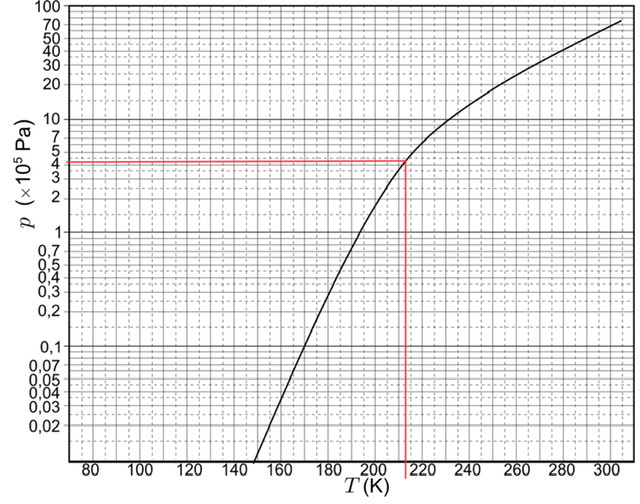
\includegraphics[width=15cm]{thermo78.jpeg}
\end{center}
\end{solution}
\begin{solution}{normal}
If the coefficient of friction $\mu$ surpasses a certain value then the block will start rolling without slipping, and in turn, will roll with a different total acceleration. This means that before finding the acceleration of the ball, we must find this coefficient of friction and break the acceleration into two cases.
\vspace{2mm}

The coefficient of friction can be found from considering the boundary case of static friction.
From
$$ma=mg\sin\theta-F_s$$and
$$I\alpha=F_sr$$we get
$$a=g\sin\theta-\frac{F_s}{m}$$and
$$\alpha=\frac{F_sr}{I}$$With static friction there is no slipping thus we combine using $a=\alpha{r}$ to get
$$F_s=\frac{mI\sin\theta}{I+mr^2}$$Since $F_s\leq{F_{s,max}}=\mu mg\cos\theta$, the angle where the "rimless wheel" stops rolling without slipping can be found as
$$\frac{mI\sin\theta}{I+mr^2}=\mu mg\cos\theta\implies \tan\theta=\mu\frac{I+mr^2}{I}$$The moment of inertia of a ball about it's central axis is $\frac{2}{5}mr^2$, so by substituting this we find
\[\mu=\frac{I}{I+mr^2}\tan\theta\implies\mu=\frac{\frac{2}{5}mr^2}{\frac{2}{5}mr^2+mr^2}\tan\theta=\frac{2}{7}\tan\theta.\]Now, we have two cases:
\vspace{2mm}

\textbf{Case 1.} $\mu>\frac{2}{7}\tan\theta$. The ball will start rolling without slipping down the ramp. We know that
\[mg\sin\theta-f=ma\]Newton’s second law of rotation gives
\[-fr=I_{\text{cm}}\alpha\implies f=\frac{-I_{\text{cm}}\alpha}{R}\]Substituting $I=\frac{2}{5}mr^2$ into this result for our equation gives us
\[f=\frac{-\left(\frac{2}{5}mr^2\right)(-a_{\text{cm}}/r)}{r}=\frac{2}{5}ma\]Taking this result back to our first equation
\[mg\sin\theta-\frac{2}{5}ma=ma\]\[a=\frac{5}{7}g\sin\theta\]
\vspace{3mm}

\textbf{Case 2.} $\mu<\frac{2}{7}\tan\theta$. The ball will simply slide down the ramp in this case, so we have
\[mg\sin\theta-\mu mg\cos\theta=ma\]\[a=g\sin\theta-\mu g\cos\theta.\]
\end{solution}

\begin{solution}{easy}
The density of some matter of mass $m$ can be given by 
\[\rho = N \frac{m}{V} \]
where $N$ is the number density of the substance. This means that for dry and humid air on each respective air can be given as 
\[\rho_d = N_d \frac{m_d}{V}, \quad N_h \frac{m_h}{V}.\]
The number density of the dry air is given by 
\[N_d = \frac{M}{M_a} = \frac{M}{28.8}\]
while the number density of the humid air will be 
\[N_h = 0.02\cdot \frac{M^{\prime}}{M_w} + 0.98\cdot \frac{M^{\prime}}{M_a} = 0.02\cdot \frac{M^{\prime}}{28.8} + 0.98\cdot \frac{M^{\prime}}{18}.\]
We can now compare the ratio of densities since we require the number density to be the same or in other words, 
\[\frac{\rho_d}{\rho_h} = \frac{N_d m_d}{N_h m_h} = \frac{\frac{M}{28.8}\cdot M^{\prime}}{M^{\prime}\cdot \left(0.02\cdot \frac{M^{\prime}}{28.8} + 0.98\cdot \frac{M^{\prime}}{18}\right)M} = \frac{1}{28.8\left(\frac{0.02}{18} + \frac{0.98}{18}\right)} = 0.9881.\]
This means that the moist air is then 
\[\rho_m = \rho_h = 0.9881 \rho_d = 1.2352\;\mathrm{kg/m^3}.\]
\end{solution}
\begin{solution}{hard} First, let us notice that the period of oscillations $T=0.01 \text{ s}$ is extremely small, so any deviation in the velocity caused by friction can be ignored if we only focus on the average velocity. We assume that the block travels at a constant velocity $u$ rightwards in the positive direction. Let us examine the movement qualitatively.
\vspace{3mm}

As the board starts moving rightwards, it is important to note that the velocity of the block relative to the board is rightwards, so the friction force $mg\mu_1$ points leftwards. This goes on for a time $t_1$ until the velocity of the board matches the velocity of the block and overtakes it. This goes on for a time $t_2$ where the board reaches a maximum and starts to slow down all the way until it has a velocity of $u$ again. During this time period, the friction force points to the right with a magnitude $mg\mu_2$. Finally, for a time $t_3=t_1$, the board is still moving towards the right but the friction force points towards the left. The total duration is $t_1+t_2+t_3=T/2$.
\vspace{3mm}

Finally, the board starts travelling in the leftwards direction. The friction force here is a constant $mg\mu_1$ directed towards the left and lasts for a time $t_4=T/2$
\vspace{3mm}

Now let's do the math. Let's work with the assumption we made that the block has a roughly constant average velocity. If this was not the case, then friction forces would either speed it up or slow it down until the motion is roughly constant. As a result, the total change in momentum, or impulse is zero. We have:
$$(-mg\mu_1)t_1+(mg\mu_2)t_2+(-mg\mu_1)t_3+(-mg\mu_1)t_4=0$$
Letting $t_1=t_3$ we get:
$$\mu_2t_2=\mu_1t_4+2\mu_1t_1$$
Having $2t_1+t_2=t_4$ then we have:
$$\mu_2(t_4-2t_1)=\mu_1t_4+2\mu_2t_1 \implies (\mu_2-\mu_1)t_4=4\mu_1t_1$$
or:
$$t_1 = \frac{(\mu_2-\mu_1)t_4}{2(\mu_2+\mu_1)}$$
Since $t_4=0.005 \text{ s}$ we get:
$$t_1 = \frac{t_4}{8}$$
this is an eighth of half a period and corresponds to the time where the board has the same velocity as the block. I put this through a visual program and determined this corresponds to $0.64 \text{ m/s}$. To one significant digit, , the average velocity of the board is $\boxed{v=0.6 \text{ m/s}}$
\end{solution}

\begin{solution}{hard}
At a temperature of $77.4\;\mathrm{K}$ (i.e. at the boiling point of nitrogen), the pressure of saturated nitrogen vapour is $1\;\mathrm{atm}$ ,while the saturated pressure of oxygen becomes $1\;\mathrm{atm}$ at a higher temperature of $90.2\;\mathrm{K}$.
\vspace{3mm}

\noindent The molar ratio of oxygen and nitrogen is $21:79$. The ratio of the partial pressures of the two components will also be very close to molar ratio, because, until the start of liquefaction, the behaviour of each gas constituent is very close to that of an ideal gas. When the partial pressure of oxygen is $0.2226\;\mathrm{atm}$, liquefaction of oxygen starts. The partial pressure of oxygen does not increase further as temperature is constant.The partial pressure of $N_2$ at the onset of oxygen liquefaction is $0.2226\times \frac{79}{21}\,\text{atm} = 0.8374\;\mathrm{atm}$. This is less than the saturated vapour pressure of nitrogen at this temperature, which, since $77.4\,\text{K}$ is nitrogen’s boiling point, has a value of $1\,\text{atm}$.Consequently, nitrogen does not liquefy at this pressure. Therefore total pressure at this point $P_1$ is $0.8374+0.2226=1.06 \,\text{atm}$. As the compression is isothermal, volume at this point $V_1$ is $1.001\times \frac{0.500}{1.06} \,\text{l} = 0.4721 \,\text{l}$. During the subsequent compression, the partial pressure of the oxygen, already in two phases, does not change, while the nitrogen pressure increases from $0.8374\,\text{atm}$ to $1.00\,\text{atm}$. This latter pressure will be reached when the volume has been reduced by a factor of $(0.8374/1.00)=0.8374$. Therefore volume at this point $V_2$ is $0.8374\times 0.4721\,\text{l} = 0.3953\,\text{l}$.After that, the total pressure remains constant (at $0.2226+1.00= 1.22\,\text{atm}$) until the liquefaction is complete, just the volume is decreased now.
\end{solution}
\begin{solution}{hard}
Note that the velocity vector in the picture is drawn wrong, it should be normal to the board.
\vspace{2mm}

Since the board is flat, we wish to move into a reference frame where the velocity of the board is parallel to its surface. We also want the stream lines of the water to be nice, so we don’t want a vertical component of the water’s velocity in the new reference frame. Thus, a reference frame moving with velocity $v/\cos\alpha$ to the left will used, where the board’s velocity is parallel to its surface (thus can be ignored) and the water is flowing horizontally.
\vspace{2mm}

The setup now is very similar to that of problem 53. The water is flowing to a wall with velocity $v/\cos\alpha$ to the right, and Bernoulli’s equation along the stream line near the surface (constant pressure, no significant change in height) tells us that the water will be directed with the same speed of $v/\cos\alpha$ and along the surface of the board.
\vspace{2mm}

Now that we have the velocity of the water in the frame of the board, we shift back to the lab frame. Adding the velocity vectors of equal magnitudes of $v/\cos\alpha$ with one horizontally to the left and one at an angle $\alpha$ from the vertical gives
$$ \vec{u} = -\left(\frac{v}{\cos{\alpha}} + v \tan{\alpha}\right)\  \hat{i} + v\ \hat{j} \Rightarrow u = v \sqrt{1+\left(\frac{1+\sin{\alpha}}{\cos{\alpha}}\right)}$$ $$ \Rightarrow u = \frac{v}{\cos{\alpha}}\sqrt{2(1+\sin{\alpha})}   = \boxed{\frac{2v}{\cos{\alpha}} \cos\left(\frac\pi 4-\frac\alpha2\right)}$$
\end{solution}

\begin{solution}{hard}
\textbf{(a)} Since the temperature is constant, we have an isothermal compression where:
$$P_0V_0=P_1V_1 \implies P_0r_0^3 = P_1r_1^3$$Since $r_1=\frac{1}{2}r_0$, we have $P_1=8P_0$.
\vspace{2mm}

\textbf{(b)} The heat generated is equal to the negative work done:
$$Q=-W=-\int P dV$$Using $PV=nRT$, we get:
$$Q=-nRT\ln\left(\frac{V_0}{V_3}\right)=\frac{3mRT_0}{\mu}\ln\left(\frac{r_0}{r_3}\right)$$
\textbf{(c)} We now have an adiabatic compression since not heat is exiting the system:
$$PV^\gamma=\text{constant} \implies TV^{\gamma-1}=\text{constant} \implies T_3=T_0\left(\frac{r_3}{r_0}\right)^{3\gamma-3}.$$
\textbf{(d)} The final radius refers to the point in which the gravitational potential energy is comparable to the thermal energy:
$$\frac{GM\mu}{r_4}=RT_0\left(\frac{r_3}{r_4}\right)^{3\gamma-3}\implies r_4=r_3\left(\frac{RT_0r_3}{\mu Gm}\right)^\frac{1}{4-3\gamma}$$and using the relationship from part (c), we get:
$$T_4=T_0\left(\frac{RT_0r_3}{\mu Gm}\right)^\frac{3\gamma-3}{4-3\gamma}$$
\end{solution}
\begin{solution}{hard}
\textbf{(a)} First, we assume that the process is reversible (even though this is not very likely). Then, the work done on the liquid is:
$$dW=(P-P_0)4\pi r^2 dR = dE_k \implies (P-P_0) R^2 dR = \frac{\rho}{2}d(r^3 \dot{r}^2)$$
The initial pressure is given by:
$$P_i=\frac{P_0R_0^3}{R_i^3}$$
so using $PV^\gamma$, we get:
$$P = P_0 \left(\frac{R_0^3}{R_i^3}\right)\left(\frac{R_i}{r}\right)^{3\gamma}$$
Since $\gamma=5/3$, this simplifies to:
$$P_0\left(49\left(\frac{R_0}{r}\right)^{5}-1\right) r^2 dr = \frac{\rho}{2}d(r^3 \dot{r}^2)$$
Integrating the left hand side, we can first make the substitution $\beta=\frac{r}{R_0}$ to simplify it to:
$$P_0R_0^3 \int_7^\alpha \left(\frac{49}{\beta^3}-\beta^2\right) d\beta = P_0R_0^3 \left(\frac{1}{2}-\frac{49}{2\alpha^2}+\frac{7^3}{3}-\frac{\alpha^3}{3}\right)$$
The right hand side evaluates to zero since it starts and ends off at rest. Thus, setting this to zero, we get the equation:
$$6\alpha^{5}+147-689\alpha^{2}$$
Making the assumption that $6\alpha^5 \ll 1$, we get a quadratic:
$$\alpha=\sqrt{\frac{147}{689}} \implies R_\text{min}=0.462R_0=2.31 \,\mathrm{\mu m}$$
We also know from $TV^{\gamma-1}$ that the maximum temperature is thus:
$$T_\text{max}=6.86 \times 10^4 \text{ K}.$$
\vspace{3mm}

\noindent \textbf{(b)} We can apply the same differential equation. The LHS stays the same, but the RHS no longer becomes zero. The RHS can be evaluated to:
$$\int_{0}^{\alpha^3\dot{\beta}^2} \frac{\rho R_0^5}{2} d(\beta^3\dot{\beta}^2)=\frac{\rho R_0^5}{2}(\alpha^3\dot{\beta}^2)$$
Setting it equal, we see that:
$$P_0R_0^3 \left(\frac{1}{2}-\frac{49}{2\alpha^2}+\frac{7^3}{3}-\frac{\alpha^3}{3}\right)=\frac{\rho R_0^5}{2}(\alpha^3\dot{\beta}^2) \implies \dot{\beta}^2 \propto \frac{689}{6\alpha^3}-\frac{49}{2\alpha^5}-\frac{1}{3}$$
This is at a maximum when:
$$\alpha=\sqrt{\frac{6\cdot5\cdot49}{2\cdot3\cdot689}}=0.596 \implies R_f=2.98 R_0$$
\vspace{3mm}

\noindent \textbf{(c)} We make the assumption that between these two times, the speed is roughly the same. The average radius is:
$$\langle R\rangle = 2.645 \,\mathrm{\mu m}$$
and thus plugging in this into our expression for $\dot{r}$ gives $\dot{r}=192.77 \text{ m/s}$ such that the total time is:
$$\Delta t= 3.48 \times 10^{-9} \text{ s}$$
\vspace{3mm}

\noindent \textbf{(d)} By Stefan-Boltzmann Law, we have that 
\[\dot{Q} = a\sigma \cdot 4\pi r^2 T^4.\]
Substituting 
\[T = T_0 \left(\frac{R_i}{r}\right)^2,\]
we result in the expression of
\[\dot{Q} = 4\pi a \sigma R_i^8 T_0^4/r^6.\]
We require that 
\[Q\leq \frac{1}{5}U\implies \left|\dot{Q}\right| \leq \left|\frac{1}{5}\dot{U}\right|\]
and therefore, we attempt to find $\dot{U}$ as well. Note that 
\[\dot{U} = -P_i \dot{V} = -P_i \left(\frac{V_i}{V}\right)^{\gamma} \dot{V} =  -4\pi P_i R_i^5 \dot{r}/r^3.\]
We now can set our expression to be 
\[\frac{4\pi a\sigma R_i^8 T_0^4}{r^6} \leq \frac{1}{5}\cdot \frac{4\pi P_i R_i^5\dot{r}}{r^3}\implies a \leq \frac{P_i r^3 \dot{r}}{5R_i^3\sigma T_0^4}\approx 0.0107\]
\end{solution}
\begin{solution}{normal}
The rod will act like a spring (since the rod is thin and made out of steel, while steel is elastic). After the left sphere has collided with the stationary sphere, the latter will acquire velocity $v_0$ and the former will stay at rest. Using momentum conservation when considering the entire system at impact, we find that,
\[(2m)v_0 = mv_0 + (2m)v_f\implies v_f = \frac{1}{2}v_0.\]
We can then compare the initial and final kinetic energies
\begin{align*}
K_i&= \frac{1}{2}(2m)v_0^2 = mv_0^2\\
K_f&= \frac{1}{2}(2m)v_f^2 + \frac{1}{2}mv_0^2 = \frac{3}{4}mv_0^2
\end{align*}
Here, we can see that kinetic energy is not conserved. However, we still do not know where this energy goes to. The dumbbell, as a system of spheres and springs, will begin oscillating around its centre of mass. After a half period the dumbbell will be too far away to expand outwards and hit the mass again. Thus, we can say that the rest of the energy is stored in the oscillating dumbbell after.
\end{solution}


\end{document}
